\documentclass[twoside]{book}

% Packages required by doxygen
\usepackage{calc}
\usepackage{doxygen}
\usepackage{graphicx}
\usepackage[utf8]{inputenc}
\usepackage{makeidx}
\usepackage{multicol}
\usepackage{multirow}
\usepackage{textcomp}
\usepackage[table]{xcolor}

% Font selection
\usepackage[T1]{fontenc}
\usepackage{mathptmx}
\usepackage[scaled=.90]{helvet}
\usepackage{courier}
\usepackage{amssymb}
\usepackage{sectsty}
\renewcommand{\familydefault}{\sfdefault}
\allsectionsfont{%
  \fontseries{bc}\selectfont%
  \color{darkgray}%
}
\renewcommand{\DoxyLabelFont}{%
  \fontseries{bc}\selectfont%
  \color{darkgray}%
}

% Page & text layout
\usepackage{geometry}
\geometry{%
  a4paper,%
  top=2.5cm,%
  bottom=2.5cm,%
  left=2.5cm,%
  right=2.5cm%
}
\tolerance=750
\hfuzz=15pt
\hbadness=750
\setlength{\emergencystretch}{15pt}
\setlength{\parindent}{0cm}
\setlength{\parskip}{0.2cm}
\makeatletter
\renewcommand{\paragraph}{%
  \@startsection{paragraph}{4}{0ex}{-1.0ex}{1.0ex}{%
    \normalfont\normalsize\bfseries\SS@parafont%
  }%
}
\renewcommand{\subparagraph}{%
  \@startsection{subparagraph}{5}{0ex}{-1.0ex}{1.0ex}{%
    \normalfont\normalsize\bfseries\SS@subparafont%
  }%
}
\makeatother

% Headers & footers
\usepackage{fancyhdr}
\pagestyle{fancyplain}
\fancyhead[LE]{\fancyplain{}{\bfseries\thepage}}
\fancyhead[CE]{\fancyplain{}{}}
\fancyhead[RE]{\fancyplain{}{\bfseries\leftmark}}
\fancyhead[LO]{\fancyplain{}{\bfseries\rightmark}}
\fancyhead[CO]{\fancyplain{}{}}
\fancyhead[RO]{\fancyplain{}{\bfseries\thepage}}
\fancyfoot[LE]{\fancyplain{}{}}
\fancyfoot[CE]{\fancyplain{}{}}
\fancyfoot[RE]{\fancyplain{}{\bfseries\scriptsize Generated on Mon Apr 27 2015 10\-:31\-:10 for My Project by Doxygen }}
\fancyfoot[LO]{\fancyplain{}{\bfseries\scriptsize Generated on Mon Apr 27 2015 10\-:31\-:10 for My Project by Doxygen }}
\fancyfoot[CO]{\fancyplain{}{}}
\fancyfoot[RO]{\fancyplain{}{}}
\renewcommand{\footrulewidth}{0.4pt}
\renewcommand{\chaptermark}[1]{%
  \markboth{#1}{}%
}
\renewcommand{\sectionmark}[1]{%
  \markright{\thesection\ #1}%
}

% Indices & bibliography
\usepackage{natbib}
\usepackage[titles]{tocloft}
\setcounter{tocdepth}{3}
\setcounter{secnumdepth}{5}
\makeindex

% Hyperlinks (required, but should be loaded last)
\usepackage{ifpdf}
\ifpdf
  \usepackage[pdftex,pagebackref=true]{hyperref}
\else
  \usepackage[ps2pdf,pagebackref=true]{hyperref}
\fi
\hypersetup{%
  colorlinks=true,%
  linkcolor=blue,%
  citecolor=blue,%
  unicode%
}

% Custom commands
\newcommand{\clearemptydoublepage}{%
  \newpage{\pagestyle{empty}\cleardoublepage}%
}


%===== C O N T E N T S =====

\begin{document}

% Titlepage & ToC
\hypersetup{pageanchor=false}
\pagenumbering{roman}
\begin{titlepage}
\vspace*{7cm}
\begin{center}%
{\Large My Project }\\
\vspace*{1cm}
{\large Generated by Doxygen 1.8.6}\\
\vspace*{0.5cm}
{\small Mon Apr 27 2015 10:31:10}\\
\end{center}
\end{titlepage}
\clearemptydoublepage
\tableofcontents
\clearemptydoublepage
\pagenumbering{arabic}
\hypersetup{pageanchor=true}

%--- Begin generated contents ---
\chapter{Hierarchical Index}
\section{Class Hierarchy}
This inheritance list is sorted roughly, but not completely, alphabetically\-:\begin{DoxyCompactList}
\item \contentsline{section}{Bezier}{\pageref{classBezier}}{}
\item \contentsline{section}{B\-Spline}{\pageref{classBSpline}}{}
\item \contentsline{section}{Catmull\-Rom}{\pageref{classCatmullRom}}{}
\item \contentsline{section}{controller\-\_\-ground\-\_\-\-G\-L}{\pageref{classcontroller__ground__GL}}{}
\item \contentsline{section}{Couleur}{\pageref{classCouleur}}{}
\item \contentsline{section}{Datapackage}{\pageref{classDatapackage}}{}
\item exception\begin{DoxyCompactList}
\item \contentsline{section}{Erreur}{\pageref{classErreur}}{}
\end{DoxyCompactList}
\item \contentsline{section}{Face}{\pageref{classFace}}{}
\item \contentsline{section}{Les\-Textures}{\pageref{classLesTextures}}{}
\item \contentsline{section}{Magicfish}{\pageref{classMagicfish}}{}
\item \contentsline{section}{Materiel}{\pageref{classMateriel}}{}
\item \contentsline{section}{model\-\_\-ground\-\_\-\-G\-L}{\pageref{classmodel__ground__GL}}{}
\item \contentsline{section}{Objet3\-D}{\pageref{classObjet3D}}{}
\begin{DoxyCompactList}
\item \contentsline{section}{Cubique}{\pageref{classCubique}}{}
\item \contentsline{section}{Sphere}{\pageref{classSphere}}{}
\item \contentsline{section}{Surface}{\pageref{classSurface}}{}
\begin{DoxyCompactList}
\item \contentsline{section}{S\-Circulaire}{\pageref{classSCirculaire}}{}
\item \contentsline{section}{S\-Lineaire}{\pageref{classSLineaire}}{}
\item \contentsline{section}{S\-Revolution}{\pageref{classSRevolution}}{}
\end{DoxyCompactList}
\item \contentsline{section}{Surface\-\_\-\-Bezier}{\pageref{classSurface__Bezier}}{}
\end{DoxyCompactList}
\item \contentsline{section}{Objets}{\pageref{classObjets}}{}
\begin{DoxyCompactList}
\item \contentsline{section}{Tore}{\pageref{classTore}}{}
\end{DoxyCompactList}
\item \contentsline{section}{Point\-G\-L}{\pageref{classPointGL}}{}
\item Q\-G\-L\-Widget\begin{DoxyCompactList}
\item \contentsline{section}{G\-L\-Widget}{\pageref{classGLWidget}}{}
\begin{DoxyCompactList}
\item \contentsline{section}{View\-\_\-ground\-\_\-\-G\-L}{\pageref{classView__ground__GL}}{}
\begin{DoxyCompactList}
\item \contentsline{section}{ground\-G\-L\-Widget}{\pageref{classgroundGLWidget}}{}
\item \contentsline{section}{View\-\_\-pcl}{\pageref{classView__pcl}}{}
\begin{DoxyCompactList}
\item \contentsline{section}{scnreader\-\_\-view}{\pageref{classscnreader__view}}{}
\end{DoxyCompactList}
\end{DoxyCompactList}
\end{DoxyCompactList}
\end{DoxyCompactList}
\item Q\-Main\-Window\begin{DoxyCompactList}
\item \contentsline{section}{Main\-Window}{\pageref{classMainWindow}}{}
\end{DoxyCompactList}
\item \contentsline{section}{Scene}{\pageref{classScene}}{}
\item \contentsline{section}{Scn\-Data}{\pageref{classScnData}}{}
\item \contentsline{section}{Texel}{\pageref{classTexel}}{}
\item \contentsline{section}{Texture}{\pageref{classTexture}}{}
\item \contentsline{section}{Tool\-Open\-C\-V}{\pageref{classToolOpenCV}}{}
\item \contentsline{section}{Tools\-P\-C\-L}{\pageref{classToolsPCL}}{}
\begin{DoxyCompactList}
\item \contentsline{section}{scnreader\-\_\-model}{\pageref{classscnreader__model}}{}
\end{DoxyCompactList}
\end{DoxyCompactList}

\chapter{Class Index}
\section{Class List}
Here are the classes, structs, unions and interfaces with brief descriptions\-:\begin{DoxyCompactList}
\item\contentsline{section}{\hyperlink{classBezier}{Bezier} }{\pageref{classBezier}}{}
\item\contentsline{section}{\hyperlink{classBSpline}{B\-Spline} }{\pageref{classBSpline}}{}
\item\contentsline{section}{\hyperlink{classCatmullRom}{Catmull\-Rom} }{\pageref{classCatmullRom}}{}
\item\contentsline{section}{\hyperlink{classcontroller__ground__GL}{controller\-\_\-ground\-\_\-\-G\-L} }{\pageref{classcontroller__ground__GL}}{}
\item\contentsline{section}{\hyperlink{classCouleur}{Couleur} }{\pageref{classCouleur}}{}
\item\contentsline{section}{\hyperlink{classCubique}{Cubique} }{\pageref{classCubique}}{}
\item\contentsline{section}{\hyperlink{classDatapackage}{Datapackage} }{\pageref{classDatapackage}}{}
\item\contentsline{section}{\hyperlink{classErreur}{Erreur} \\*for manage exeptions This class is used for throw a custom exeption }{\pageref{classErreur}}{}
\item\contentsline{section}{\hyperlink{classFace}{Face} }{\pageref{classFace}}{}
\item\contentsline{section}{\hyperlink{classGLWidget}{G\-L\-Widget} }{\pageref{classGLWidget}}{}
\item\contentsline{section}{\hyperlink{classgroundGLWidget}{ground\-G\-L\-Widget} \\*This class grouped the main function open\-G\-L. Each function is already implemented and allows easy use of open\-G\-L . For more functionalities, You could overloading each function into a new class }{\pageref{classgroundGLWidget}}{}
\item\contentsline{section}{\hyperlink{classLesTextures}{Les\-Textures} }{\pageref{classLesTextures}}{}
\item\contentsline{section}{\hyperlink{classMagicfish}{Magicfish} }{\pageref{classMagicfish}}{}
\item\contentsline{section}{\hyperlink{classMainWindow}{Main\-Window} }{\pageref{classMainWindow}}{}
\item\contentsline{section}{\hyperlink{classMateriel}{Materiel} }{\pageref{classMateriel}}{}
\item\contentsline{section}{\hyperlink{classmodel__ground__GL}{model\-\_\-ground\-\_\-\-G\-L} }{\pageref{classmodel__ground__GL}}{}
\item\contentsline{section}{\hyperlink{classObjet3D}{Objet3\-D} }{\pageref{classObjet3D}}{}
\item\contentsline{section}{\hyperlink{classObjets}{Objets} }{\pageref{classObjets}}{}
\item\contentsline{section}{\hyperlink{classPointGL}{Point\-G\-L} }{\pageref{classPointGL}}{}
\item\contentsline{section}{\hyperlink{classScene}{Scene} }{\pageref{classScene}}{}
\item\contentsline{section}{\hyperlink{classSCirculaire}{S\-Circulaire} }{\pageref{classSCirculaire}}{}
\item\contentsline{section}{\hyperlink{classScnData}{Scn\-Data} }{\pageref{classScnData}}{}
\item\contentsline{section}{\hyperlink{classscnreader__model}{scnreader\-\_\-model} }{\pageref{classscnreader__model}}{}
\item\contentsline{section}{\hyperlink{classscnreader__view}{scnreader\-\_\-view} }{\pageref{classscnreader__view}}{}
\item\contentsline{section}{\hyperlink{classSLineaire}{S\-Lineaire} }{\pageref{classSLineaire}}{}
\item\contentsline{section}{\hyperlink{classSphere}{Sphere} }{\pageref{classSphere}}{}
\item\contentsline{section}{\hyperlink{classSRevolution}{S\-Revolution} }{\pageref{classSRevolution}}{}
\item\contentsline{section}{\hyperlink{classSurface}{Surface} }{\pageref{classSurface}}{}
\item\contentsline{section}{\hyperlink{classSurface__Bezier}{Surface\-\_\-\-Bezier} }{\pageref{classSurface__Bezier}}{}
\item\contentsline{section}{\hyperlink{classTexel}{Texel} }{\pageref{classTexel}}{}
\item\contentsline{section}{\hyperlink{classTexture}{Texture} }{\pageref{classTexture}}{}
\item\contentsline{section}{\hyperlink{classToolOpenCV}{Tool\-Open\-C\-V} \\*Interface entre open\-C\-V et Qt }{\pageref{classToolOpenCV}}{}
\item\contentsline{section}{\hyperlink{classToolsPCL}{Tools\-P\-C\-L} \\*for manage pcl This class is used to loading, reading and processing of point clouds }{\pageref{classToolsPCL}}{}
\item\contentsline{section}{\hyperlink{classTore}{Tore} }{\pageref{classTore}}{}
\item\contentsline{section}{\hyperlink{classView__ground__GL}{View\-\_\-ground\-\_\-\-G\-L} }{\pageref{classView__ground__GL}}{}
\item\contentsline{section}{\hyperlink{classView__pcl}{View\-\_\-pcl} }{\pageref{classView__pcl}}{}
\end{DoxyCompactList}

\chapter{File Index}
\section{File List}
Here is a list of all documented files with brief descriptions\-:\begin{DoxyCompactList}
\item\contentsline{section}{{\bfseries mainwindow.\-h} }{\pageref{mainwindow_8h}}{}
\item\contentsline{section}{modules/exceptions/\hyperlink{erreur_8h}{erreur.\-h} \\*File to the managements of exeptions }{\pageref{erreur_8h}}{}
\item\contentsline{section}{modules/open\-C\-V/{\bfseries magicfish.\-h} }{\pageref{magicfish_8h}}{}
\item\contentsline{section}{modules/open\-C\-V/ground/model/{\bfseries toolopencv.\-h} }{\pageref{toolopencv_8h}}{}
\item\contentsline{section}{modules/open\-G\-L/ground/\hyperlink{groundglwidget_8h}{groundglwidget.\-h} \\*File to the managements of exeptions }{\pageref{groundglwidget_8h}}{}
\item\contentsline{section}{modules/open\-G\-L/ground/controller/{\bfseries controller\-\_\-ground\-\_\-gl.\-h} }{\pageref{controller__ground__gl_8h}}{}
\item\contentsline{section}{modules/open\-G\-L/ground/model/{\bfseries G\-L\-Widget.\-h} }{\pageref{GLWidget_8h}}{}
\item\contentsline{section}{modules/open\-G\-L/ground/model/{\bfseries Les\-Textures.\-h} }{\pageref{LesTextures_8h}}{}
\item\contentsline{section}{modules/open\-G\-L/ground/model/{\bfseries Materiel.\-h} }{\pageref{Materiel_8h}}{}
\item\contentsline{section}{modules/open\-G\-L/ground/model/{\bfseries model\-\_\-ground\-\_\-gl.\-h} }{\pageref{model__ground__gl_8h}}{}
\item\contentsline{section}{modules/open\-G\-L/ground/model/{\bfseries Scene.\-h} }{\pageref{Scene_8h}}{}
\item\contentsline{section}{modules/open\-G\-L/ground/model/{\bfseries Texture.\-h} }{\pageref{Texture_8h}}{}
\item\contentsline{section}{modules/open\-G\-L/ground/view/{\bfseries view\-\_\-ground\-\_\-\-G\-L.\-h} }{\pageref{view__ground__GL_8h}}{}
\item\contentsline{section}{modules/open\-G\-L/tools\-\_\-models/{\bfseries Couleur.\-h} }{\pageref{Couleur_8h}}{}
\item\contentsline{section}{modules/open\-G\-L/tools\-\_\-models/{\bfseries Face.\-h} }{\pageref{Face_8h}}{}
\item\contentsline{section}{modules/open\-G\-L/tools\-\_\-models/{\bfseries Objet3\-D.\-h} }{\pageref{Objet3D_8h}}{}
\item\contentsline{section}{modules/open\-G\-L/tools\-\_\-models/{\bfseries Objets.\-h} }{\pageref{Objets_8h}}{}
\item\contentsline{section}{modules/open\-G\-L/tools\-\_\-models/{\bfseries Point.\-h} }{\pageref{Point_8h}}{}
\item\contentsline{section}{modules/open\-G\-L/tools\-\_\-models/{\bfseries Texel.\-h} }{\pageref{Texel_8h}}{}
\item\contentsline{section}{modules/open\-G\-L/tools\-\_\-models/\-Courbes/{\bfseries Bezier.\-h} }{\pageref{Bezier_8h}}{}
\item\contentsline{section}{modules/open\-G\-L/tools\-\_\-models/\-Courbes/{\bfseries B\-Spline.\-h} }{\pageref{BSpline_8h}}{}
\item\contentsline{section}{modules/open\-G\-L/tools\-\_\-models/\-Courbes/{\bfseries Catmull\-Rom.\-h} }{\pageref{CatmullRom_8h}}{}
\item\contentsline{section}{modules/open\-G\-L/tools\-\_\-models/objets/{\bfseries Cubique.\-h} }{\pageref{Cubique_8h}}{}
\item\contentsline{section}{modules/open\-G\-L/tools\-\_\-models/objets/{\bfseries Sphere.\-h} }{\pageref{Sphere_8h}}{}
\item\contentsline{section}{modules/open\-G\-L/tools\-\_\-models/objets/{\bfseries Tore.\-h} }{\pageref{Tore_8h}}{}
\item\contentsline{section}{modules/open\-G\-L/tools\-\_\-models/\-Surfaces/{\bfseries S\-Circulaire.\-h} }{\pageref{SCirculaire_8h}}{}
\item\contentsline{section}{modules/open\-G\-L/tools\-\_\-models/\-Surfaces/{\bfseries S\-Lineaire.\-h} }{\pageref{SLineaire_8h}}{}
\item\contentsline{section}{modules/open\-G\-L/tools\-\_\-models/\-Surfaces/{\bfseries S\-Revolution.\-h} }{\pageref{SRevolution_8h}}{}
\item\contentsline{section}{modules/open\-G\-L/tools\-\_\-models/\-Surfaces/{\bfseries Surface.\-h} }{\pageref{Surface_8h}}{}
\item\contentsline{section}{modules/open\-G\-L/tools\-\_\-models/\-Surfaces/{\bfseries Surface\-\_\-\-Bezier.\-h} }{\pageref{Surface__Bezier_8h}}{}
\item\contentsline{section}{modules/pcl/ground/\hyperlink{ToolsPCL_8h}{Tools\-P\-C\-L.\-h} \\*File to the managements of pcl }{\pageref{ToolsPCL_8h}}{}
\item\contentsline{section}{modules/pcl/view/{\bfseries view\-\_\-pcl.\-h} }{\pageref{view__pcl_8h}}{}
\item\contentsline{section}{works/{\bfseries datapackage.\-h} }{\pageref{datapackage_8h}}{}
\item\contentsline{section}{works/{\bfseries scndata.\-h} }{\pageref{scndata_8h}}{}
\item\contentsline{section}{works/{\bfseries scnreader\-\_\-model.\-h} }{\pageref{scnreader__model_8h}}{}
\item\contentsline{section}{works/{\bfseries scnreader\-\_\-view.\-h} }{\pageref{scnreader__view_8h}}{}
\end{DoxyCompactList}

\chapter{Class Documentation}
\hypertarget{classBezier}{\section{Bezier Class Reference}
\label{classBezier}\index{Bezier@{Bezier}}
}


{\ttfamily \#include $<$Bezier.\-h$>$}

\subsection*{Public Member Functions}
\begin{DoxyCompactItemize}
\item 
\hyperlink{classBezier_a4a7be5dfa4ae95eb978123b256681c59}{Bezier} (int n)
\begin{DoxyCompactList}\small\item\em Constructeur d'une courbe type Bézier. \end{DoxyCompactList}\item 
\hypertarget{classBezier_a042d3cca85d534451938671d5d7a7383}{\hyperlink{classBezier_a042d3cca85d534451938671d5d7a7383}{Bezier} (const \hyperlink{classBezier}{Bezier} \&orig)}\label{classBezier_a042d3cca85d534451938671d5d7a7383}

\begin{DoxyCompactList}\small\item\em Constructeur de copie. \end{DoxyCompactList}\item 
\hypertarget{classBezier_a32f81ea72bd31a4607b4168839ea8815}{virtual \hyperlink{classBezier_a32f81ea72bd31a4607b4168839ea8815}{$\sim$\-Bezier} ()}\label{classBezier_a32f81ea72bd31a4607b4168839ea8815}

\begin{DoxyCompactList}\small\item\em Destructeur de la classe qui détruit tous les pointeurs. \end{DoxyCompactList}\item 
void \hyperlink{classBezier_a3973f77432e3a02a7971d6a524668aef}{Trace} (std\-::vector$<$ \hyperlink{classPointGL}{Point\-G\-L} $\ast$ $>$ P)
\begin{DoxyCompactList}\small\item\em Fonction permettant de créer la courbe, en remplissant le vecteur de points Points. \end{DoxyCompactList}\item 
\hypertarget{classBezier_a66d2cf118a768281f51ee743774b184c}{void \hyperlink{classBezier_a66d2cf118a768281f51ee743774b184c}{Affichage} ()}\label{classBezier_a66d2cf118a768281f51ee743774b184c}

\begin{DoxyCompactList}\small\item\em Fonction permettant l'affichage de la courbe. \end{DoxyCompactList}\item 
std\-::vector$<$ \hyperlink{classPointGL}{Point\-G\-L} $\ast$ $>$ \hyperlink{classBezier_ac428660e18d25b27a4e60b911c10320e}{get\-P} ()
\begin{DoxyCompactList}\small\item\em accesseur en lecture au vecteur de points contenant les points de la courbe \end{DoxyCompactList}\end{DoxyCompactItemize}


\subsection{Detailed Description}
\begin{DoxyAuthor}{Author}
P\-O\-N\-C\-I\-A\-N\-O Jean-\/\-Jacques et P\-R\-U\-D\-H\-O\-M\-M\-E Claire 
\end{DoxyAuthor}
\begin{DoxyDate}{Date}
13/03/2014
\end{DoxyDate}
Cette oeuvre, création, code, site ou texte est sous licence Creative Commons Attribution -\/ Pas d’\-Utilisation Commerciale -\/ Partage dans les Mêmes Conditions 4.\-0 International. Pour accéder à une copie de cette licence, merci de vous rendre à l'adresse suivante \href{http://creativecommons.org/licenses/by-nc-sa/4.0/deed.fr}{\tt http\-://creativecommons.\-org/licenses/by-\/nc-\/sa/4.\-0/deed.\-fr} ou envoyez un courrier à Creative Commons, 444 Castro Street, Suite 900, Mountain View, California, 94041, U\-S\-A. Copyright 2014

Contact\-: \href{mailto:ponciano.jeanjacques@gmail.com}{\tt ponciano.\-jeanjacques@gmail.\-com} 

\subsection{Constructor \& Destructor Documentation}
\hypertarget{classBezier_a4a7be5dfa4ae95eb978123b256681c59}{\index{Bezier@{Bezier}!Bezier@{Bezier}}
\index{Bezier@{Bezier}!Bezier@{Bezier}}
\subsubsection[{Bezier}]{\setlength{\rightskip}{0pt plus 5cm}Bezier\-::\-Bezier (
\begin{DoxyParamCaption}
\item[{int}]{n}
\end{DoxyParamCaption}
)}}\label{classBezier_a4a7be5dfa4ae95eb978123b256681c59}


Constructeur d'une courbe type Bézier. 


\begin{DoxyParams}{Parameters}
{\em n} & nombre de points voulu pour la courbe\\
\hline
\end{DoxyParams}
\begin{DoxyAuthor}{Author}
P\-O\-N\-C\-I\-A\-N\-O Jean-\/\-Jacques et P\-R\-U\-D\-H\-O\-M\-M\-E Claire Copyright 2014 P\-O\-N\-C\-I\-A\-N\-O Jean-\/\-Jacques et P\-R\-U\-D\-H\-O\-M\-M\-E Claire Contact\-: \href{mailto:ponciano.jeanjacques@gmail.com}{\tt ponciano.\-jeanjacques@gmail.\-com} Créé le 13 Mars 2014
\end{DoxyAuthor}
Cette oeuvre, création, code, site ou texte est sous licence Creative Commons Attribution -\/ Pas d’\-Utilisation Commerciale -\/ Partage dans les Mêmes Conditions 4.\-0 International. Pour accéder à une copie de cette licence, merci de vous rendre à l'adresse suivante \href{http://creativecommons.org/licenses/by-nc-sa/4.0/deed.fr}{\tt http\-://creativecommons.\-org/licenses/by-\/nc-\/sa/4.\-0/deed.\-fr} ou envoyez un courrier à Creative Commons, 444 Castro Street, Suite 900, Mountain View, California, 94041, U\-S\-A. 

\subsection{Member Function Documentation}
\hypertarget{classBezier_ac428660e18d25b27a4e60b911c10320e}{\index{Bezier@{Bezier}!get\-P@{get\-P}}
\index{get\-P@{get\-P}!Bezier@{Bezier}}
\subsubsection[{get\-P}]{\setlength{\rightskip}{0pt plus 5cm}std\-::vector$<$ {\bf Point\-G\-L} $\ast$ $>$ Bezier\-::get\-P (
\begin{DoxyParamCaption}
{}
\end{DoxyParamCaption}
)}}\label{classBezier_ac428660e18d25b27a4e60b911c10320e}


accesseur en lecture au vecteur de points contenant les points de la courbe 

\begin{DoxyReturn}{Returns}
le vecteur de points Points 
\end{DoxyReturn}
\hypertarget{classBezier_a3973f77432e3a02a7971d6a524668aef}{\index{Bezier@{Bezier}!Trace@{Trace}}
\index{Trace@{Trace}!Bezier@{Bezier}}
\subsubsection[{Trace}]{\setlength{\rightskip}{0pt plus 5cm}void Bezier\-::\-Trace (
\begin{DoxyParamCaption}
\item[{std\-::vector$<$ {\bf Point\-G\-L} $\ast$ $>$}]{P}
\end{DoxyParamCaption}
)}}\label{classBezier_a3973f77432e3a02a7971d6a524668aef}


Fonction permettant de créer la courbe, en remplissant le vecteur de points Points. 


\begin{DoxyParams}{Parameters}
{\em P} & vecteur contenant les points de contrôle de la courbe nécessaires à sa construction \\
\hline
\end{DoxyParams}


The documentation for this class was generated from the following files\-:\begin{DoxyCompactItemize}
\item 
modules/open\-G\-L/tools\-\_\-models/\-Courbes/Bezier.\-h\item 
modules/open\-G\-L/tools\-\_\-models/\-Courbes/Bezier.\-cpp\end{DoxyCompactItemize}

\hypertarget{classBSpline}{\section{B\-Spline Class Reference}
\label{classBSpline}\index{B\-Spline@{B\-Spline}}
}


{\ttfamily \#include $<$B\-Spline.\-h$>$}

\subsection*{Public Member Functions}
\begin{DoxyCompactItemize}
\item 
\hyperlink{classBSpline_a270bffd29442d124a0a063502c0f1f37}{B\-Spline} (int nb)
\begin{DoxyCompactList}\small\item\em Constructeur d'une courbe type B-\/\-Spline. \end{DoxyCompactList}\item 
\hypertarget{classBSpline_a7c86b59f6e656ecc3c78ef4e1f35ca98}{\hyperlink{classBSpline_a7c86b59f6e656ecc3c78ef4e1f35ca98}{B\-Spline} (const \hyperlink{classBSpline}{B\-Spline} \&orig)}\label{classBSpline_a7c86b59f6e656ecc3c78ef4e1f35ca98}

\begin{DoxyCompactList}\small\item\em Constructeur de copie. \end{DoxyCompactList}\item 
\hypertarget{classBSpline_a535039ab5127dc644a1a121faedf88b3}{virtual \hyperlink{classBSpline_a535039ab5127dc644a1a121faedf88b3}{$\sim$\-B\-Spline} ()}\label{classBSpline_a535039ab5127dc644a1a121faedf88b3}

\begin{DoxyCompactList}\small\item\em Destructeur de la classe qui détruit tous les pointeurs. \end{DoxyCompactList}\item 
void \hyperlink{classBSpline_a21eed7e5829622d86020706210532bd3}{Trace} (std\-::vector$<$ \hyperlink{classPointGL}{Point\-G\-L} $\ast$ $>$ P)
\begin{DoxyCompactList}\small\item\em Fonction permettant de créer la courbe, en remplissant le vecteur de points Points. \end{DoxyCompactList}\item 
\hypertarget{classBSpline_a81e035fc5c4b4748e2ba24ea0a60db1b}{void \hyperlink{classBSpline_a81e035fc5c4b4748e2ba24ea0a60db1b}{Affichage} ()}\label{classBSpline_a81e035fc5c4b4748e2ba24ea0a60db1b}

\begin{DoxyCompactList}\small\item\em Fonction permettant l'affichage de la courbe. \end{DoxyCompactList}\item 
std\-::vector$<$ \hyperlink{classPointGL}{Point\-G\-L} $\ast$ $>$ \hyperlink{classBSpline_aa4606c8de89943ddea85f7065d5cb2fa}{get\-P} ()
\begin{DoxyCompactList}\small\item\em accesseur en lecture au vecteur de points contenant les points de la courbe \end{DoxyCompactList}\end{DoxyCompactItemize}


\subsection{Detailed Description}
\begin{DoxyAuthor}{Author}
P\-O\-N\-C\-I\-A\-N\-O Jean-\/\-Jacques et P\-R\-U\-D\-H\-O\-M\-M\-E Claire 
\end{DoxyAuthor}
\begin{DoxyDate}{Date}
13/03/2014
\end{DoxyDate}
Cette oeuvre, création, code, site ou texte est sous licence Creative Commons Attribution -\/ Pas d’\-Utilisation Commerciale -\/ Partage dans les Mêmes Conditions 4.\-0 International. Pour accéder à une copie de cette licence, merci de vous rendre à l'adresse suivante \href{http://creativecommons.org/licenses/by-nc-sa/4.0/deed.fr}{\tt http\-://creativecommons.\-org/licenses/by-\/nc-\/sa/4.\-0/deed.\-fr} ou envoyez un courrier à Creative Commons, 444 Castro Street, Suite 900, Mountain View, California, 94041, U\-S\-A. Copyright 2014

Contact\-: \href{mailto:ponciano.jeanjacques@gmail.com}{\tt ponciano.\-jeanjacques@gmail.\-com} 

\subsection{Constructor \& Destructor Documentation}
\hypertarget{classBSpline_a270bffd29442d124a0a063502c0f1f37}{\index{B\-Spline@{B\-Spline}!B\-Spline@{B\-Spline}}
\index{B\-Spline@{B\-Spline}!BSpline@{B\-Spline}}
\subsubsection[{B\-Spline}]{\setlength{\rightskip}{0pt plus 5cm}B\-Spline\-::\-B\-Spline (
\begin{DoxyParamCaption}
\item[{int}]{nb}
\end{DoxyParamCaption}
)}}\label{classBSpline_a270bffd29442d124a0a063502c0f1f37}


Constructeur d'une courbe type B-\/\-Spline. 


\begin{DoxyParams}{Parameters}
{\em nb} & nombre de points voulu pour la courbe \\
\hline
\end{DoxyParams}


\subsection{Member Function Documentation}
\hypertarget{classBSpline_aa4606c8de89943ddea85f7065d5cb2fa}{\index{B\-Spline@{B\-Spline}!get\-P@{get\-P}}
\index{get\-P@{get\-P}!BSpline@{B\-Spline}}
\subsubsection[{get\-P}]{\setlength{\rightskip}{0pt plus 5cm}std\-::vector$<$ {\bf Point\-G\-L} $\ast$ $>$ B\-Spline\-::get\-P (
\begin{DoxyParamCaption}
{}
\end{DoxyParamCaption}
)}}\label{classBSpline_aa4606c8de89943ddea85f7065d5cb2fa}


accesseur en lecture au vecteur de points contenant les points de la courbe 

\begin{DoxyReturn}{Returns}
le vecteur de points Points 
\end{DoxyReturn}
\hypertarget{classBSpline_a21eed7e5829622d86020706210532bd3}{\index{B\-Spline@{B\-Spline}!Trace@{Trace}}
\index{Trace@{Trace}!BSpline@{B\-Spline}}
\subsubsection[{Trace}]{\setlength{\rightskip}{0pt plus 5cm}void B\-Spline\-::\-Trace (
\begin{DoxyParamCaption}
\item[{std\-::vector$<$ {\bf Point\-G\-L} $\ast$ $>$}]{P}
\end{DoxyParamCaption}
)}}\label{classBSpline_a21eed7e5829622d86020706210532bd3}


Fonction permettant de créer la courbe, en remplissant le vecteur de points Points. 


\begin{DoxyParams}{Parameters}
{\em P} & vecteur contenant les points de contrôle de la courbe nécessaires à sa construction \\
\hline
\end{DoxyParams}


The documentation for this class was generated from the following files\-:\begin{DoxyCompactItemize}
\item 
modules/open\-G\-L/tools\-\_\-models/\-Courbes/B\-Spline.\-h\item 
modules/open\-G\-L/tools\-\_\-models/\-Courbes/B\-Spline.\-cpp\end{DoxyCompactItemize}

\hypertarget{classCatmullRom}{\section{Catmull\-Rom Class Reference}
\label{classCatmullRom}\index{Catmull\-Rom@{Catmull\-Rom}}
}


{\ttfamily \#include $<$Catmull\-Rom.\-h$>$}

\subsection*{Public Member Functions}
\begin{DoxyCompactItemize}
\item 
\hyperlink{classCatmullRom_ac0e994d7a9644541cf02e8fd82fa0773}{Catmull\-Rom} (float s, int n)
\begin{DoxyCompactList}\small\item\em Constructeur d'une courbe type Catmull-\/\-Rom. \end{DoxyCompactList}\item 
\hypertarget{classCatmullRom_a1acf3961c850ce0f7911b64db3463629}{\hyperlink{classCatmullRom_a1acf3961c850ce0f7911b64db3463629}{Catmull\-Rom} (const \hyperlink{classCatmullRom}{Catmull\-Rom} \&orig)}\label{classCatmullRom_a1acf3961c850ce0f7911b64db3463629}

\begin{DoxyCompactList}\small\item\em Constructeur de copie. \end{DoxyCompactList}\item 
\hypertarget{classCatmullRom_a5661b43985801f9adf5047f057b55ddc}{virtual \hyperlink{classCatmullRom_a5661b43985801f9adf5047f057b55ddc}{$\sim$\-Catmull\-Rom} ()}\label{classCatmullRom_a5661b43985801f9adf5047f057b55ddc}

\begin{DoxyCompactList}\small\item\em Destructeur de la classe qui détruit tous les pointeurs. \end{DoxyCompactList}\item 
void \hyperlink{classCatmullRom_a2be4505724c40d8bc7d7d72164ab5585}{trace} (std\-::vector$<$ \hyperlink{classPointGL}{Point\-G\-L} $\ast$ $>$ P)
\begin{DoxyCompactList}\small\item\em Fonction permettant de créer la courbe, en remplissant le vecteur de points Points. \end{DoxyCompactList}\item 
void \hyperlink{classCatmullRom_ac70e97a3222e3883d1df1c74ede347a8}{set\-Inds} (float s)
\begin{DoxyCompactList}\small\item\em accesseur en écriture au vecteur de points contenant les points de la courbe \end{DoxyCompactList}\item 
\hypertarget{classCatmullRom_a9d20a2042b439a8d129481185f5c57fa}{void \hyperlink{classCatmullRom_a9d20a2042b439a8d129481185f5c57fa}{affichage} ()}\label{classCatmullRom_a9d20a2042b439a8d129481185f5c57fa}

\begin{DoxyCompactList}\small\item\em Fonction permettant l'affichage de la courbe. \end{DoxyCompactList}\item 
std\-::vector$<$ \hyperlink{classPointGL}{Point\-G\-L} $\ast$ $>$ \hyperlink{classCatmullRom_a6921464048064a19dd08e4fced1b88ff}{get\-P} ()
\begin{DoxyCompactList}\small\item\em accesseur en lecture au vecteur de points contenant les points de la courbe \end{DoxyCompactList}\end{DoxyCompactItemize}


\subsection{Detailed Description}
\begin{DoxyAuthor}{Author}
P\-O\-N\-C\-I\-A\-N\-O Jean-\/\-Jacques et P\-R\-U\-D\-H\-O\-M\-M\-E Claire 
\end{DoxyAuthor}
\begin{DoxyDate}{Date}
13/03/2014
\end{DoxyDate}
Cette oeuvre, création, code, site ou texte est sous licence Creative Commons Attribution -\/ Pas d’\-Utilisation Commerciale -\/ Partage dans les Mêmes Conditions 4.\-0 International. Pour accéder à une copie de cette licence, merci de vous rendre à l'adresse suivante \href{http://creativecommons.org/licenses/by-nc-sa/4.0/deed.fr}{\tt http\-://creativecommons.\-org/licenses/by-\/nc-\/sa/4.\-0/deed.\-fr} ou envoyez un courrier à Creative Commons, 444 Castro Street, Suite 900, Mountain View, California, 94041, U\-S\-A. Copyright 2014

Contact\-: \href{mailto:ponciano.jeanjacques@gmail.com}{\tt ponciano.\-jeanjacques@gmail.\-com} 

\subsection{Constructor \& Destructor Documentation}
\hypertarget{classCatmullRom_ac0e994d7a9644541cf02e8fd82fa0773}{\index{Catmull\-Rom@{Catmull\-Rom}!Catmull\-Rom@{Catmull\-Rom}}
\index{Catmull\-Rom@{Catmull\-Rom}!CatmullRom@{Catmull\-Rom}}
\subsubsection[{Catmull\-Rom}]{\setlength{\rightskip}{0pt plus 5cm}Catmull\-Rom\-::\-Catmull\-Rom (
\begin{DoxyParamCaption}
\item[{float}]{s, }
\item[{int}]{n}
\end{DoxyParamCaption}
)}}\label{classCatmullRom_ac0e994d7a9644541cf02e8fd82fa0773}


Constructeur d'une courbe type Catmull-\/\-Rom. 


\begin{DoxyParams}{Parameters}
{\em s} & coefficient de la courbe (en générale, égale à 1/2) \\
\hline
{\em n} & nombre de points voulu pour la courbe \\
\hline
\end{DoxyParams}


\subsection{Member Function Documentation}
\hypertarget{classCatmullRom_a6921464048064a19dd08e4fced1b88ff}{\index{Catmull\-Rom@{Catmull\-Rom}!get\-P@{get\-P}}
\index{get\-P@{get\-P}!CatmullRom@{Catmull\-Rom}}
\subsubsection[{get\-P}]{\setlength{\rightskip}{0pt plus 5cm}std\-::vector$<$ {\bf Point\-G\-L} $\ast$ $>$ Catmull\-Rom\-::get\-P (
\begin{DoxyParamCaption}
{}
\end{DoxyParamCaption}
)}}\label{classCatmullRom_a6921464048064a19dd08e4fced1b88ff}


accesseur en lecture au vecteur de points contenant les points de la courbe 

\begin{DoxyReturn}{Returns}
le vecteur de points Points 
\end{DoxyReturn}
\hypertarget{classCatmullRom_ac70e97a3222e3883d1df1c74ede347a8}{\index{Catmull\-Rom@{Catmull\-Rom}!set\-Inds@{set\-Inds}}
\index{set\-Inds@{set\-Inds}!CatmullRom@{Catmull\-Rom}}
\subsubsection[{set\-Inds}]{\setlength{\rightskip}{0pt plus 5cm}void Catmull\-Rom\-::set\-Inds (
\begin{DoxyParamCaption}
\item[{float}]{s}
\end{DoxyParamCaption}
)}}\label{classCatmullRom_ac70e97a3222e3883d1df1c74ede347a8}


accesseur en écriture au vecteur de points contenant les points de la courbe 


\begin{DoxyParams}{Parameters}
{\em s} & coefficient de la courbe (en générale, égale à 1/2) \\
\hline
\end{DoxyParams}
\hypertarget{classCatmullRom_a2be4505724c40d8bc7d7d72164ab5585}{\index{Catmull\-Rom@{Catmull\-Rom}!trace@{trace}}
\index{trace@{trace}!CatmullRom@{Catmull\-Rom}}
\subsubsection[{trace}]{\setlength{\rightskip}{0pt plus 5cm}void Catmull\-Rom\-::trace (
\begin{DoxyParamCaption}
\item[{std\-::vector$<$ {\bf Point\-G\-L} $\ast$ $>$}]{P}
\end{DoxyParamCaption}
)}}\label{classCatmullRom_a2be4505724c40d8bc7d7d72164ab5585}


Fonction permettant de créer la courbe, en remplissant le vecteur de points Points. 


\begin{DoxyParams}{Parameters}
{\em P} & vecteur contenant les points de contrôle de la courbe nécessaires à sa construction \\
\hline
\end{DoxyParams}


The documentation for this class was generated from the following files\-:\begin{DoxyCompactItemize}
\item 
modules/open\-G\-L/tools\-\_\-models/\-Courbes/Catmull\-Rom.\-h\item 
modules/open\-G\-L/tools\-\_\-models/\-Courbes/Catmull\-Rom.\-cpp\end{DoxyCompactItemize}

\hypertarget{classcontroller__ground__GL}{\section{controller\-\_\-ground\-\_\-\-G\-L Class Reference}
\label{classcontroller__ground__GL}\index{controller\-\_\-ground\-\_\-\-G\-L@{controller\-\_\-ground\-\_\-\-G\-L}}
}
\subsection*{Public Member Functions}
\begin{DoxyCompactItemize}
\item 
\hypertarget{classcontroller__ground__GL_a5e2c2ca1e696c4629e0c4cf647b4d150}{{\bfseries controller\-\_\-ground\-\_\-\-G\-L} (\hyperlink{classmodel__ground__GL}{model\-\_\-ground\-\_\-\-G\-L} $\ast$model)}\label{classcontroller__ground__GL_a5e2c2ca1e696c4629e0c4cf647b4d150}

\item 
\hypertarget{classcontroller__ground__GL_a88f9f5a5e3546516c96a71f7f3d08867}{void {\bfseries initialize\-G\-L} ()}\label{classcontroller__ground__GL_a88f9f5a5e3546516c96a71f7f3d08867}

\item 
\hypertarget{classcontroller__ground__GL_aa955e96f368cfbf2bb9daba3019c2fb4}{void {\bfseries key\-Press\-Event} (Q\-Key\-Event $\ast$key\-Event)}\label{classcontroller__ground__GL_aa955e96f368cfbf2bb9daba3019c2fb4}

\item 
\hypertarget{classcontroller__ground__GL_af4873b68ac38eb386f3359b2d8207ef9}{void {\bfseries mouse\-Press\-Event} (Q\-Mouse\-Event $\ast$event)}\label{classcontroller__ground__GL_af4873b68ac38eb386f3359b2d8207ef9}

\item 
\hypertarget{classcontroller__ground__GL_a08720d4fdcb1dd125d7c28fd37c15222}{void {\bfseries mouse\-Release\-Event} (Q\-Mouse\-Event $\ast$event)}\label{classcontroller__ground__GL_a08720d4fdcb1dd125d7c28fd37c15222}

\item 
\hypertarget{classcontroller__ground__GL_aa0db8cdc102837daaaf635362cf9c747}{void {\bfseries mouse\-Move\-Event} (Q\-Mouse\-Event $\ast$event)}\label{classcontroller__ground__GL_aa0db8cdc102837daaaf635362cf9c747}

\item 
\hypertarget{classcontroller__ground__GL_a2936e71b98a38b66e3fa09afe1538506}{void {\bfseries zoom} ()}\label{classcontroller__ground__GL_a2936e71b98a38b66e3fa09afe1538506}

\item 
\hypertarget{classcontroller__ground__GL_a747914c093fc33b5c4e3f25b71ef0fb1}{void {\bfseries dezoom} ()}\label{classcontroller__ground__GL_a747914c093fc33b5c4e3f25b71ef0fb1}

\end{DoxyCompactItemize}


The documentation for this class was generated from the following files\-:\begin{DoxyCompactItemize}
\item 
modules/open\-G\-L/ground/controller/controller\-\_\-ground\-\_\-gl.\-h\item 
modules/open\-G\-L/ground/controller/controller\-\_\-ground\-\_\-gl.\-cpp\end{DoxyCompactItemize}

\hypertarget{classCouleur}{\section{Couleur Class Reference}
\label{classCouleur}\index{Couleur@{Couleur}}
}


{\ttfamily \#include $<$Couleur.\-h$>$}

\subsection*{Public Member Functions}
\begin{DoxyCompactItemize}
\item 
\hyperlink{classCouleur_a687a457edb08b51dbcd0299bb0b6a882}{Couleur} ()
\item 
\hyperlink{classCouleur_a1e16a48a6dbc76b76d47a516d5848a63}{Couleur} (float r, float g, float b)
\item 
\hypertarget{classCouleur_a3d1b0342753548700d886f85ab286616}{{\bfseries Couleur} (const \hyperlink{classCouleur}{Couleur} \&orig)}\label{classCouleur_a3d1b0342753548700d886f85ab286616}

\item 
\hypertarget{classCouleur_a5cf13a9fb92983ec10791860a4aaafa0}{float {\bfseries get\-R} () const }\label{classCouleur_a5cf13a9fb92983ec10791860a4aaafa0}

\item 
\hypertarget{classCouleur_a4dbd817480b34bb393cf99729642190f}{float {\bfseries get\-G} () const }\label{classCouleur_a4dbd817480b34bb393cf99729642190f}

\item 
\hypertarget{classCouleur_ae8445c1a512aafcb6624aa2f62150162}{float {\bfseries get\-B} () const }\label{classCouleur_ae8445c1a512aafcb6624aa2f62150162}

\end{DoxyCompactItemize}


\subsection{Detailed Description}
\begin{DoxyAuthor}{Author}
P\-O\-N\-C\-I\-A\-N\-O Jean-\/\-Jacques et P\-R\-U\-D\-H\-O\-M\-M\-E Claire 
\end{DoxyAuthor}
\begin{DoxyDate}{Date}
13/03/2014
\end{DoxyDate}
Cette oeuvre, création, code, site ou texte est sous licence Creative Commons Attribution -\/ Pas d’\-Utilisation Commerciale -\/ Partage dans les Mêmes Conditions 4.\-0 International. Pour accéder à une copie de cette licence, merci de vous rendre à l'adresse suivante \href{http://creativecommons.org/licenses/by-nc-sa/4.0/deed.fr}{\tt http\-://creativecommons.\-org/licenses/by-\/nc-\/sa/4.\-0/deed.\-fr} ou envoyez un courrier à Creative Commons, 444 Castro Street, Suite 900, Mountain View, California, 94041, U\-S\-A. Copyright 2014

Contact\-: \href{mailto:ponciano.jeanjacques@gmail.com}{\tt ponciano.\-jeanjacques@gmail.\-com} 

\subsection{Constructor \& Destructor Documentation}
\hypertarget{classCouleur_a687a457edb08b51dbcd0299bb0b6a882}{\index{Couleur@{Couleur}!Couleur@{Couleur}}
\index{Couleur@{Couleur}!Couleur@{Couleur}}
\subsubsection[{Couleur}]{\setlength{\rightskip}{0pt plus 5cm}Couleur\-::\-Couleur (
\begin{DoxyParamCaption}
{}
\end{DoxyParamCaption}
)}}\label{classCouleur_a687a457edb08b51dbcd0299bb0b6a882}
Construit une couleur blanche \hypertarget{classCouleur_a1e16a48a6dbc76b76d47a516d5848a63}{\index{Couleur@{Couleur}!Couleur@{Couleur}}
\index{Couleur@{Couleur}!Couleur@{Couleur}}
\subsubsection[{Couleur}]{\setlength{\rightskip}{0pt plus 5cm}Couleur\-::\-Couleur (
\begin{DoxyParamCaption}
\item[{float}]{r, }
\item[{float}]{g, }
\item[{float}]{b}
\end{DoxyParamCaption}
)}}\label{classCouleur_a1e16a48a6dbc76b76d47a516d5848a63}
Construction de la couleur rgb 
\begin{DoxyParams}{Parameters}
{\em r} & canal rouge \\
\hline
{\em g} & canal vert \\
\hline
{\em b} & canal bleu \\
\hline
\end{DoxyParams}


The documentation for this class was generated from the following files\-:\begin{DoxyCompactItemize}
\item 
modules/open\-G\-L/tools\-\_\-models/Couleur.\-h\item 
modules/open\-G\-L/tools\-\_\-models/Couleur.\-cpp\end{DoxyCompactItemize}

\hypertarget{classCubique}{\section{Cubique Class Reference}
\label{classCubique}\index{Cubique@{Cubique}}
}


{\ttfamily \#include $<$Cubique.\-h$>$}

Inheritance diagram for Cubique\-:\begin{figure}[H]
\begin{center}
\leavevmode
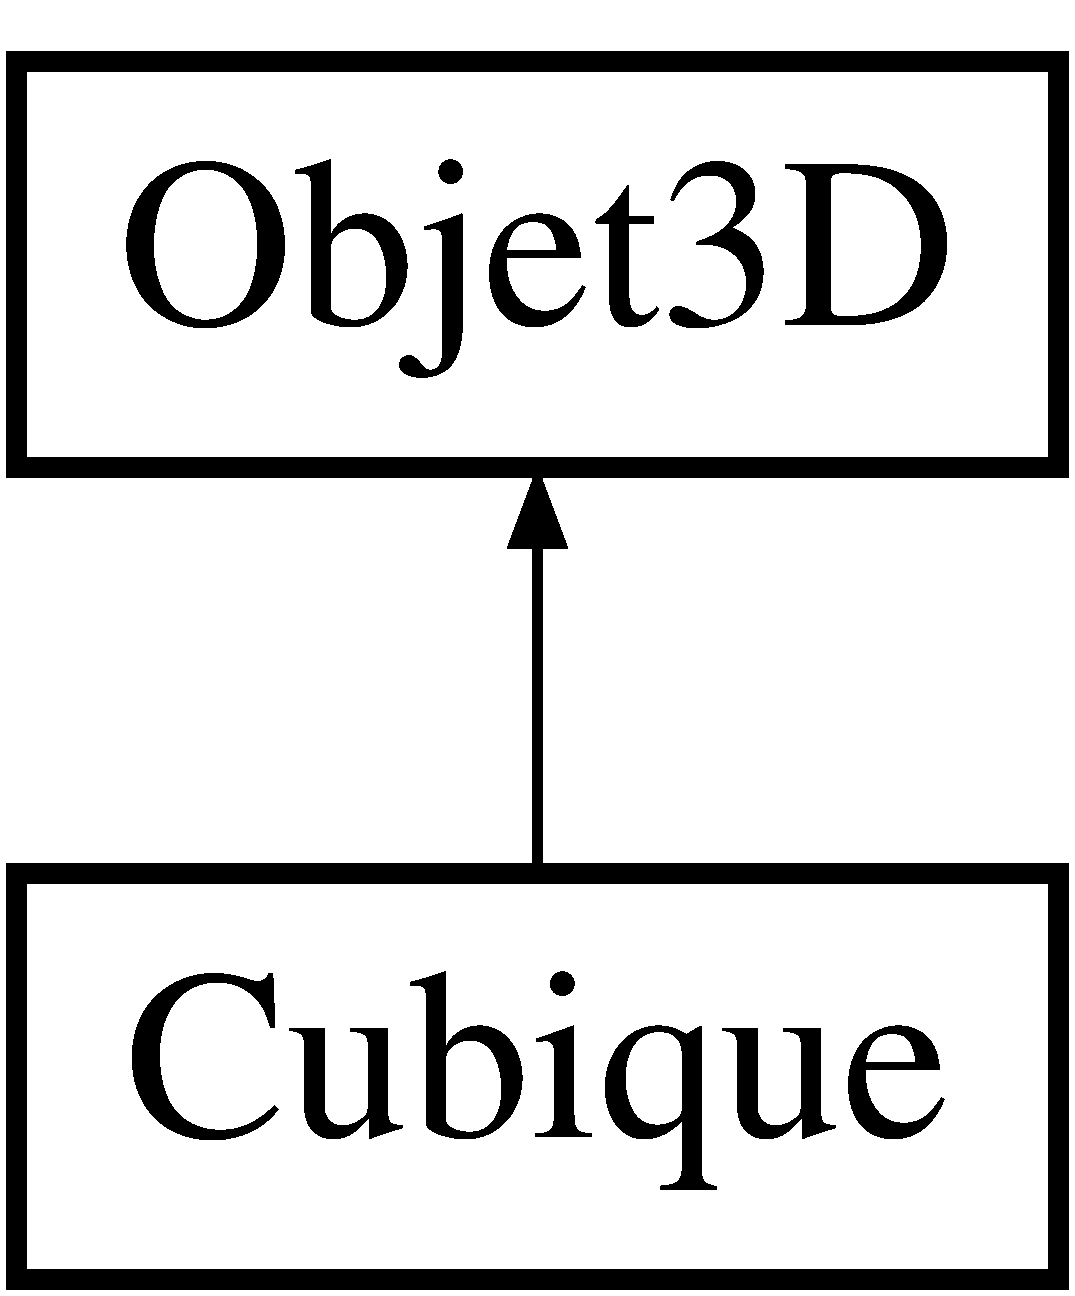
\includegraphics[height=2.000000cm]{classCubique}
\end{center}
\end{figure}
\subsection*{Public Member Functions}
\begin{DoxyCompactItemize}
\item 
\hyperlink{classCubique_a01a053ef2fad8dcb5a50ad1a3c809efe}{Cubique} (float largeur, float hauteur, float longueur, \hyperlink{classTexture}{Texture} $\ast$d, \hyperlink{classTexture}{Texture} $\ast$f, \hyperlink{classTexture}{Texture} $\ast$autre)
\item 
\hypertarget{classCubique_aa0045d5d037f086aaf3d584eea922149}{{\bfseries Cubique} (const \hyperlink{classCubique}{Cubique} \&orig)}\label{classCubique_aa0045d5d037f086aaf3d584eea922149}

\item 
void \hyperlink{classCubique_aa84591f1589b4f5cf4eafd7d98ebec50}{affichage} ()
\end{DoxyCompactItemize}
\subsection*{Additional Inherited Members}


\subsection{Detailed Description}
\begin{DoxyAuthor}{Author}
P\-O\-N\-C\-I\-A\-N\-O Jean-\/\-Jacques et P\-R\-U\-D\-H\-O\-M\-M\-E Claire 
\end{DoxyAuthor}
\begin{DoxyDate}{Date}
13/03/2014
\end{DoxyDate}
Cette oeuvre, création, code, site ou texte est sous licence Creative Commons Attribution -\/ Pas d’\-Utilisation Commerciale -\/ Partage dans les Mêmes Conditions 4.\-0 International. Pour accéder à une copie de cette licence, merci de vous rendre à l'adresse suivante \href{http://creativecommons.org/licenses/by-nc-sa/4.0/deed.fr}{\tt http\-://creativecommons.\-org/licenses/by-\/nc-\/sa/4.\-0/deed.\-fr} ou envoyez un courrier à Creative Commons, 444 Castro Street, Suite 900, Mountain View, California, 94041, U\-S\-A. Copyright 2014

Contact\-: \href{mailto:ponciano.jeanjacques@gmail.com}{\tt ponciano.\-jeanjacques@gmail.\-com} 

\subsection{Constructor \& Destructor Documentation}
\hypertarget{classCubique_a01a053ef2fad8dcb5a50ad1a3c809efe}{\index{Cubique@{Cubique}!Cubique@{Cubique}}
\index{Cubique@{Cubique}!Cubique@{Cubique}}
\subsubsection[{Cubique}]{\setlength{\rightskip}{0pt plus 5cm}Cubique\-::\-Cubique (
\begin{DoxyParamCaption}
\item[{float}]{largeur, }
\item[{float}]{hauteur, }
\item[{float}]{longueur, }
\item[{{\bf Texture} $\ast$}]{d, }
\item[{{\bf Texture} $\ast$}]{f, }
\item[{{\bf Texture} $\ast$}]{autre}
\end{DoxyParamCaption}
)}}\label{classCubique_a01a053ef2fad8dcb5a50ad1a3c809efe}
Construteur d'un objet sous forme de cube texturé 
\begin{DoxyParams}{Parameters}
{\em largeur} & largeur de l'objet \\
\hline
{\em hauteur} & hauteur de l'objet \\
\hline
{\em longueur} & longueur de l'objet \\
\hline
{\em d} & texture à appliquer sur le dessus \\
\hline
{\em f} & texture à appliquer sur le devant \\
\hline
{\em autre} & texture à appliquer sur les autres côtés \\
\hline
\end{DoxyParams}


\subsection{Member Function Documentation}
\hypertarget{classCubique_aa84591f1589b4f5cf4eafd7d98ebec50}{\index{Cubique@{Cubique}!affichage@{affichage}}
\index{affichage@{affichage}!Cubique@{Cubique}}
\subsubsection[{affichage}]{\setlength{\rightskip}{0pt plus 5cm}void Cubique\-::affichage (
\begin{DoxyParamCaption}
{}
\end{DoxyParamCaption}
)}}\label{classCubique_aa84591f1589b4f5cf4eafd7d98ebec50}
Affichage de l'objet 

The documentation for this class was generated from the following files\-:\begin{DoxyCompactItemize}
\item 
modules/open\-G\-L/tools\-\_\-models/objets/Cubique.\-h\item 
modules/open\-G\-L/tools\-\_\-models/objets/Cubique.\-cpp\end{DoxyCompactItemize}

\hypertarget{classDatapackage}{\section{Datapackage Class Reference}
\label{classDatapackage}\index{Datapackage@{Datapackage}}
}
\subsection*{Public Member Functions}
\begin{DoxyCompactItemize}
\item 
\hypertarget{classDatapackage_a25969cd74b7b4ecbafd0e622677821cb}{{\bfseries Datapackage} (Q\-Byte\-Array datas, int start)}\label{classDatapackage_a25969cd74b7b4ecbafd0e622677821cb}

\item 
\hypertarget{classDatapackage_a907b7ec8ca3b802bf8d041b645306b10}{void {\bfseries read\-Data\-File} (std\-::string pathname)}\label{classDatapackage_a907b7ec8ca3b802bf8d041b645306b10}

\item 
\hypertarget{classDatapackage_a69e500a0bdfb3086ab164d7b08a19af8}{std\-::string {\bfseries to\-String} ()}\label{classDatapackage_a69e500a0bdfb3086ab164d7b08a19af8}

\item 
\hypertarget{classDatapackage_a69f2633667d6665a8e5a9e25bde93c1d}{virtual void {\bfseries Print} (std\-::ostream \&O) const }\label{classDatapackage_a69f2633667d6665a8e5a9e25bde93c1d}

\item 
\hypertarget{classDatapackage_abaa431b4807d967d0b7ab5515f08edcf}{pcl\-::\-Point\-Cloud$<$ pcl\-::\-Point\-X\-Y\-Z $>$\\*
\-::Ptr {\bfseries get\-Cloud} () const }\label{classDatapackage_abaa431b4807d967d0b7ab5515f08edcf}

\item 
\hypertarget{classDatapackage_abc1ad9b2f943a6d467726dda778595cb}{void {\bfseries set\-Cloud} (const pcl\-::\-Point\-Cloud$<$ pcl\-::\-Point\-X\-Y\-Z $>$\-::Ptr \&value)}\label{classDatapackage_abc1ad9b2f943a6d467726dda778595cb}

\item 
\hypertarget{classDatapackage_ac077faf854d6a3f6d5a608afd5b05364}{Q\-String {\bfseries get\-Id} () const }\label{classDatapackage_ac077faf854d6a3f6d5a608afd5b05364}

\item 
\hypertarget{classDatapackage_a3ffb4caf156e1f7dbadd70995acf1838}{void {\bfseries set\-Id} (const Q\-String \&value)}\label{classDatapackage_a3ffb4caf156e1f7dbadd70995acf1838}

\item 
\hypertarget{classDatapackage_a2668dc4c59aa862dc2d8ceed0491950e}{Q\-String {\bfseries get\-Version} () const }\label{classDatapackage_a2668dc4c59aa862dc2d8ceed0491950e}

\item 
\hypertarget{classDatapackage_abb4b106237a40d77a88f08c4b100430d}{void {\bfseries set\-Version} (const Q\-String \&value)}\label{classDatapackage_abb4b106237a40d77a88f08c4b100430d}

\item 
\hypertarget{classDatapackage_a2ddb140dae8c664c5427a79e28235619}{int {\bfseries get\-Radius} () const }\label{classDatapackage_a2ddb140dae8c664c5427a79e28235619}

\item 
\hypertarget{classDatapackage_aebfb1f2a09ca9d0628fb68e5dce20256}{void {\bfseries set\-Radius} (const int \&value)}\label{classDatapackage_aebfb1f2a09ca9d0628fb68e5dce20256}

\item 
\hypertarget{classDatapackage_a367c1575e48ab1b9d9e8c6f390574b0a}{int {\bfseries get\-Radienkorrektur} () const }\label{classDatapackage_a367c1575e48ab1b9d9e8c6f390574b0a}

\item 
\hypertarget{classDatapackage_a97de6e1959e391c6adf93404c0acf9c4}{void {\bfseries set\-Radienkorrektur} (const int \&value)}\label{classDatapackage_a97de6e1959e391c6adf93404c0acf9c4}

\item 
\hypertarget{classDatapackage_aec66f542acb81cc764d1610eb9114d6e}{int {\bfseries get\-Spurweite} () const }\label{classDatapackage_aec66f542acb81cc764d1610eb9114d6e}

\item 
\hypertarget{classDatapackage_a13ca1962c331a68e2d17f0b6ab4c463d}{void {\bfseries set\-Spurweite} (const int \&value)}\label{classDatapackage_a13ca1962c331a68e2d17f0b6ab4c463d}

\item 
\hypertarget{classDatapackage_a9f1178b918e1f5ba0dc05ab63ce8bbf7}{int {\bfseries get\-Ngl\-Left\-Horizontal} () const }\label{classDatapackage_a9f1178b918e1f5ba0dc05ab63ce8bbf7}

\item 
\hypertarget{classDatapackage_a9f5cfd9d6b90af25d5578094f1500dac}{void {\bfseries set\-Ngl\-Left\-Horizontal} (const int \&value)}\label{classDatapackage_a9f5cfd9d6b90af25d5578094f1500dac}

\item 
\hypertarget{classDatapackage_a6c4c0264794960adfa3eaee8915fbca4}{int {\bfseries get\-Ngl\-Left\-Vertical} () const }\label{classDatapackage_a6c4c0264794960adfa3eaee8915fbca4}

\item 
\hypertarget{classDatapackage_a7f4292e52c6593fb6a7f945bbe43d676}{void {\bfseries set\-Ngl\-Left\-Vertical} (const int \&value)}\label{classDatapackage_a7f4292e52c6593fb6a7f945bbe43d676}

\item 
\hypertarget{classDatapackage_a6d23507972fa51bdea5bbbec1bba9f2a}{int {\bfseries get\-Ngl\-Left\-Banking} () const }\label{classDatapackage_a6d23507972fa51bdea5bbbec1bba9f2a}

\item 
\hypertarget{classDatapackage_aba24fae055a6787a81b99c81e22f9bfd}{void {\bfseries set\-Ngl\-Left\-Banking} (const int \&value)}\label{classDatapackage_aba24fae055a6787a81b99c81e22f9bfd}

\item 
\hypertarget{classDatapackage_a10f585ca2766a946d699d6cb7b8e4778}{int {\bfseries get\-Ngl\-Left\-Gauge} () const }\label{classDatapackage_a10f585ca2766a946d699d6cb7b8e4778}

\item 
\hypertarget{classDatapackage_a74476d803f2e78fba816912c94216fcb}{void {\bfseries set\-Ngl\-Left\-Gauge} (const int \&value)}\label{classDatapackage_a74476d803f2e78fba816912c94216fcb}

\item 
\hypertarget{classDatapackage_a96c30884f05365f32d11ab45f98746a2}{int {\bfseries get\-Ngl\-Right\-Horizontal} () const }\label{classDatapackage_a96c30884f05365f32d11ab45f98746a2}

\item 
\hypertarget{classDatapackage_af2051e2ec406cd5721850bfac7871e6d}{void {\bfseries set\-Ngl\-Right\-Horizontal} (const int \&value)}\label{classDatapackage_af2051e2ec406cd5721850bfac7871e6d}

\item 
\hypertarget{classDatapackage_acefd0e7c889cc8d95323dd0f26753dc5}{int {\bfseries get\-Ngl\-Right\-Vertical} () const }\label{classDatapackage_acefd0e7c889cc8d95323dd0f26753dc5}

\item 
\hypertarget{classDatapackage_aa614672aabf5684b4d4832c9368a240b}{void {\bfseries set\-Ngl\-Right\-Vertical} (const int \&value)}\label{classDatapackage_aa614672aabf5684b4d4832c9368a240b}

\item 
\hypertarget{classDatapackage_a08f8cbb9982d62be35cc136ac0572f32}{int {\bfseries get\-Ngl\-Right\-Banking} () const }\label{classDatapackage_a08f8cbb9982d62be35cc136ac0572f32}

\item 
\hypertarget{classDatapackage_ac4fd59abddf395ad388d5655b2c9f11c}{void {\bfseries set\-Ngl\-Right\-Banking} (const int \&value)}\label{classDatapackage_ac4fd59abddf395ad388d5655b2c9f11c}

\item 
\hypertarget{classDatapackage_a519c74c74ff0ba425c331a46710c4272}{int {\bfseries get\-Ngl\-Right\-Gauge} () const }\label{classDatapackage_a519c74c74ff0ba425c331a46710c4272}

\item 
\hypertarget{classDatapackage_a52e4c6d14809f20dccd1e2ffba21827e}{void {\bfseries set\-Ngl\-Right\-Gauge} (const int \&value)}\label{classDatapackage_a52e4c6d14809f20dccd1e2ffba21827e}

\item 
\hypertarget{classDatapackage_a746b186c1f8293a39866ae7e89bd1915}{int {\bfseries get\-Point\-Count} () const }\label{classDatapackage_a746b186c1f8293a39866ae7e89bd1915}

\item 
\hypertarget{classDatapackage_aa2fa86907ea6cc19f16f4ecf5553a39a}{void {\bfseries set\-Point\-Count} (const int \&value)}\label{classDatapackage_aa2fa86907ea6cc19f16f4ecf5553a39a}

\item 
\hypertarget{classDatapackage_a8e1cd6fcc6cf979190b41dfe98065563}{int {\bfseries get\-End} () const }\label{classDatapackage_a8e1cd6fcc6cf979190b41dfe98065563}

\item 
\hypertarget{classDatapackage_abfef2d431bf688a23cf9cd8654aabf6e}{void {\bfseries set\-End} (int value)}\label{classDatapackage_abfef2d431bf688a23cf9cd8654aabf6e}

\item 
\hypertarget{classDatapackage_a19d6efa99fb9a217950f67ee26951097}{int {\bfseries get\-Structuresize} () const }\label{classDatapackage_a19d6efa99fb9a217950f67ee26951097}

\item 
\hypertarget{classDatapackage_a1ede7123986211b5a28ee35d0e1ad329}{void {\bfseries set\-Structuresize} (int value)}\label{classDatapackage_a1ede7123986211b5a28ee35d0e1ad329}

\item 
\hypertarget{classDatapackage_a0de5f4d73a9d8e33c9b817462bd340bf}{int {\bfseries get\-Footpulse} () const }\label{classDatapackage_a0de5f4d73a9d8e33c9b817462bd340bf}

\item 
\hypertarget{classDatapackage_abebf5c2641e3b0223318791e86936a3a}{void {\bfseries set\-Footpulse} (int value)}\label{classDatapackage_abebf5c2641e3b0223318791e86936a3a}

\item 
\hypertarget{classDatapackage_a28c2d73d6d15bdd3635941b981f978bb}{Q\-Vector$<$ int $>$ {\bfseries get\-Distance} () const }\label{classDatapackage_a28c2d73d6d15bdd3635941b981f978bb}

\item 
\hypertarget{classDatapackage_a2507cd1bcd5717ad06d89be62a169251}{void {\bfseries set\-Distance} (const Q\-Vector$<$ int $>$ \&value)}\label{classDatapackage_a2507cd1bcd5717ad06d89be62a169251}

\item 
\hypertarget{classDatapackage_a9c9a0bd967182db48f9bbb884c57232b}{Q\-Vector$<$ int $>$ {\bfseries get\-Intensity} () const }\label{classDatapackage_a9c9a0bd967182db48f9bbb884c57232b}

\item 
\hypertarget{classDatapackage_a2031be7b427a8b9e0ff2d4c6085b0061}{void {\bfseries set\-Intensity} (const Q\-Vector$<$ int $>$ \&value)}\label{classDatapackage_a2031be7b427a8b9e0ff2d4c6085b0061}

\end{DoxyCompactItemize}
\subsection*{Friends}
\begin{DoxyCompactItemize}
\item 
\hypertarget{classDatapackage_a090ef798bfd6ea5aa522acadb4406f08}{std\-::ostream \& {\bfseries operator$<$$<$} (std\-::ostream \&O, const \hyperlink{classDatapackage}{Datapackage} \&B)}\label{classDatapackage_a090ef798bfd6ea5aa522acadb4406f08}

\end{DoxyCompactItemize}


The documentation for this class was generated from the following files\-:\begin{DoxyCompactItemize}
\item 
works/datapackage.\-h\item 
works/datapackage.\-cpp\end{DoxyCompactItemize}

\hypertarget{classErreur}{\section{Erreur Class Reference}
\label{classErreur}\index{Erreur@{Erreur}}
}


The \hyperlink{classErreur}{Erreur} class for manage exeptions This class is used for throw a custom exeption.  




{\ttfamily \#include $<$erreur.\-h$>$}

Inheritance diagram for Erreur\-:\begin{figure}[H]
\begin{center}
\leavevmode
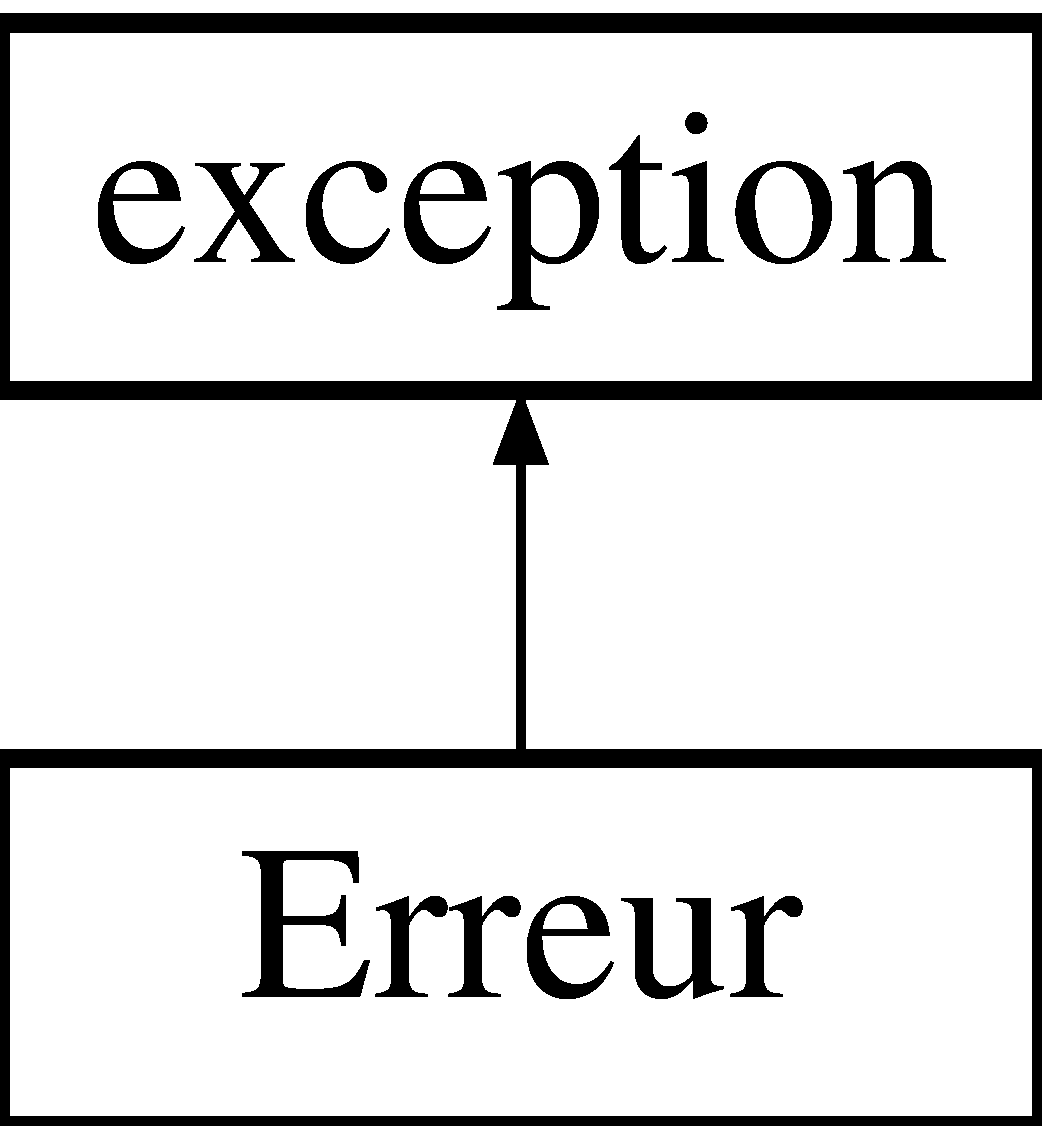
\includegraphics[height=2.000000cm]{classErreur}
\end{center}
\end{figure}
\subsection*{Public Member Functions}
\begin{DoxyCompactItemize}
\item 
\hyperlink{classErreur_a0d19b48536f8dbe265041bdc77446fca}{Erreur} (std\-::string const \&phrase=\char`\"{}error detected\char`\"{})  throw ()
\begin{DoxyCompactList}\small\item\em \hyperlink{classErreur}{Erreur} create exeption. \end{DoxyCompactList}\item 
\hypertarget{classErreur_a03f509dfcd70553d533a58ffb9db7cb6}{virtual const char $\ast$ {\bfseries what} () const   throw ()}\label{classErreur_a03f509dfcd70553d533a58ffb9db7cb6}

\end{DoxyCompactItemize}


\subsection{Detailed Description}
The \hyperlink{classErreur}{Erreur} class for manage exeptions This class is used for throw a custom exeption. 

For example, if you want throw a exeption and catch it\-:


\begin{DoxyCode}
\textcolor{keywordflow}{try}\{

\textcolor{keywordflow}{throw} \hyperlink{classErreur_a0d19b48536f8dbe265041bdc77446fca}{Erreur}(\textcolor{stringliteral}{"Description of exeption"});

\}\textcolor{keywordflow}{catch}(std::exception \textcolor{keyword}{const}& e)\{
 QMessageBox::critical(\textcolor{keyword}{this}, \textcolor{stringliteral}{"Error"}, e.what());
\}
\end{DoxyCode}
 

\subsection{Constructor \& Destructor Documentation}
\hypertarget{classErreur_a0d19b48536f8dbe265041bdc77446fca}{\index{Erreur@{Erreur}!Erreur@{Erreur}}
\index{Erreur@{Erreur}!Erreur@{Erreur}}
\subsubsection[{Erreur}]{\setlength{\rightskip}{0pt plus 5cm}Erreur\-::\-Erreur (
\begin{DoxyParamCaption}
\item[{std\-::string const \&}]{phrase = {\ttfamily \char`\"{}error~detected\char`\"{}}}
\end{DoxyParamCaption}
) throw  ) }}\label{classErreur_a0d19b48536f8dbe265041bdc77446fca}


\hyperlink{classErreur}{Erreur} create exeption. 


\begin{DoxyParams}{Parameters}
{\em phrase} & sentence explaining the reasons for the throwing of exceptions \\
\hline
\end{DoxyParams}


The documentation for this class was generated from the following files\-:\begin{DoxyCompactItemize}
\item 
modules/exceptions/\hyperlink{erreur_8h}{erreur.\-h}\item 
modules/exceptions/erreur.\-cpp\end{DoxyCompactItemize}

\hypertarget{classFace}{\section{Face Class Reference}
\label{classFace}\index{Face@{Face}}
}


{\ttfamily \#include $<$Face.\-h$>$}

\subsection*{Public Member Functions}
\begin{DoxyCompactItemize}
\item 
\hyperlink{classFace_afdb634bc2d5287ba0d62e46b57e9dc2e}{Face} ()
\item 
\hyperlink{classFace_a88e0725fb26500f174570372df28d6bf}{Face} (const \hyperlink{classFace}{Face} \&orig)
\item 
void \hyperlink{classFace_af060c26d3c550669b1796df41f08aed0}{add} (\hyperlink{classPointGL}{Point\-G\-L} $\ast$p, \hyperlink{classTexel}{Texel} $\ast$t)
\item 
void \hyperlink{classFace_a18e74dbfbb4bde83cc890c1664ce094b}{remove} ()
\item 
void \hyperlink{classFace_aaef76e86d3cc05d4ffe0fd34ae711a3b}{set\-Couleur} (float r, float g, float b)
\item 
void \hyperlink{classFace_a89341dffe04ab3d4ce3f64ea48039e54}{set\-Couleur} (const \hyperlink{classCouleur}{Couleur} \&c)
\item 
void \hyperlink{classFace_a624ad3f0698d8ece2db54edce2f1497a}{afficher} (bool lisage)
\item 
void \hyperlink{classFace_a3a318395a3017afbec8704e8fb0df918}{afficher\-Points} ()
\item 
bool \hyperlink{classFace_a2deb053f5ffee2ed5393ef39754466cf}{contain} (\hyperlink{classPointGL}{Point\-G\-L} $\ast$p) const 
\item 
std\-::vector$<$ float $>$ \hyperlink{classFace_a75e299e2d14ba3f888272edd9a8c866f}{get\-Normal} () const 
\end{DoxyCompactItemize}


\subsection{Detailed Description}
\begin{DoxyAuthor}{Author}
P\-O\-N\-C\-I\-A\-N\-O Jean-\/\-Jacques et P\-R\-U\-D\-H\-O\-M\-M\-E Claire 
\end{DoxyAuthor}
\begin{DoxyDate}{Date}
13/03/2014
\end{DoxyDate}
Cette oeuvre, création, code, site ou texte est sous licence Creative Commons Attribution -\/ Pas d’\-Utilisation Commerciale -\/ Partage dans les Mêmes Conditions 4.\-0 International. Pour accéder à une copie de cette licence, merci de vous rendre à l'adresse suivante \href{http://creativecommons.org/licenses/by-nc-sa/4.0/deed.fr}{\tt http\-://creativecommons.\-org/licenses/by-\/nc-\/sa/4.\-0/deed.\-fr} ou envoyez un courrier à Creative Commons, 444 Castro Street, Suite 900, Mountain View, California, 94041, U\-S\-A. Copyright 2014

Contact\-: \href{mailto:ponciano.jeanjacques@gmail.com}{\tt ponciano.\-jeanjacques@gmail.\-com} 

\subsection{Constructor \& Destructor Documentation}
\hypertarget{classFace_afdb634bc2d5287ba0d62e46b57e9dc2e}{\index{Face@{Face}!Face@{Face}}
\index{Face@{Face}!Face@{Face}}
\subsubsection[{Face}]{\setlength{\rightskip}{0pt plus 5cm}Face\-::\-Face (
\begin{DoxyParamCaption}
{}
\end{DoxyParamCaption}
)}}\label{classFace_afdb634bc2d5287ba0d62e46b57e9dc2e}
Constructeur \hypertarget{classFace_a88e0725fb26500f174570372df28d6bf}{\index{Face@{Face}!Face@{Face}}
\index{Face@{Face}!Face@{Face}}
\subsubsection[{Face}]{\setlength{\rightskip}{0pt plus 5cm}Face\-::\-Face (
\begin{DoxyParamCaption}
\item[{const {\bf Face} \&}]{orig}
\end{DoxyParamCaption}
)}}\label{classFace_a88e0725fb26500f174570372df28d6bf}
Constructeur de copie 
\begin{DoxyParams}{Parameters}
{\em orig} & face à copier \\
\hline
\end{DoxyParams}
\begin{DoxyReturn}{Returns}
renvoie la face copiée 
\end{DoxyReturn}


\subsection{Member Function Documentation}
\hypertarget{classFace_af060c26d3c550669b1796df41f08aed0}{\index{Face@{Face}!add@{add}}
\index{add@{add}!Face@{Face}}
\subsubsection[{add}]{\setlength{\rightskip}{0pt plus 5cm}void Face\-::add (
\begin{DoxyParamCaption}
\item[{{\bf Point\-G\-L} $\ast$}]{p, }
\item[{{\bf Texel} $\ast$}]{t}
\end{DoxyParamCaption}
)}}\label{classFace_af060c26d3c550669b1796df41f08aed0}
Ajout un point à la face 
\begin{DoxyParams}{Parameters}
{\em p} & point à ajouter \\
\hline
\end{DoxyParams}
\hypertarget{classFace_a624ad3f0698d8ece2db54edce2f1497a}{\index{Face@{Face}!afficher@{afficher}}
\index{afficher@{afficher}!Face@{Face}}
\subsubsection[{afficher}]{\setlength{\rightskip}{0pt plus 5cm}void Face\-::afficher (
\begin{DoxyParamCaption}
\item[{bool}]{lisage}
\end{DoxyParamCaption}
)}}\label{classFace_a624ad3f0698d8ece2db54edce2f1497a}
Affiche la face en couleur 
\begin{DoxyCode}
\textcolor{comment}{//affichage avec lissage de phong:}
 \hyperlink{classFace_a624ad3f0698d8ece2db54edce2f1497a}{afficher}(\textcolor{keyword}{true});
\end{DoxyCode}
 
\begin{DoxyParams}{Parameters}
{\em lisage} & affiche avec ou sans le lissage \\
\hline
\end{DoxyParams}
\hypertarget{classFace_a3a318395a3017afbec8704e8fb0df918}{\index{Face@{Face}!afficher\-Points@{afficher\-Points}}
\index{afficher\-Points@{afficher\-Points}!Face@{Face}}
\subsubsection[{afficher\-Points}]{\setlength{\rightskip}{0pt plus 5cm}void Face\-::afficher\-Points (
\begin{DoxyParamCaption}
{}
\end{DoxyParamCaption}
)}}\label{classFace_a3a318395a3017afbec8704e8fb0df918}
Affiche les points de la face \hypertarget{classFace_a2deb053f5ffee2ed5393ef39754466cf}{\index{Face@{Face}!contain@{contain}}
\index{contain@{contain}!Face@{Face}}
\subsubsection[{contain}]{\setlength{\rightskip}{0pt plus 5cm}bool Face\-::contain (
\begin{DoxyParamCaption}
\item[{{\bf Point\-G\-L} $\ast$}]{p}
\end{DoxyParamCaption}
) const}}\label{classFace_a2deb053f5ffee2ed5393ef39754466cf}
Test si le point p appartient à la face 
\begin{DoxyParams}{Parameters}
{\em p} & point à tester \\
\hline
\end{DoxyParams}
\begin{DoxyReturn}{Returns}
vrai si le point appartient à la face, faux sinon 
\end{DoxyReturn}
\hypertarget{classFace_a75e299e2d14ba3f888272edd9a8c866f}{\index{Face@{Face}!get\-Normal@{get\-Normal}}
\index{get\-Normal@{get\-Normal}!Face@{Face}}
\subsubsection[{get\-Normal}]{\setlength{\rightskip}{0pt plus 5cm}std\-::vector$<$ float $>$ Face\-::get\-Normal (
\begin{DoxyParamCaption}
{}
\end{DoxyParamCaption}
) const}}\label{classFace_a75e299e2d14ba3f888272edd9a8c866f}
Récupération du vecteur normal à la face \begin{DoxyReturn}{Returns}
le vecteur normal à la face 
\end{DoxyReturn}
\hypertarget{classFace_a18e74dbfbb4bde83cc890c1664ce094b}{\index{Face@{Face}!remove@{remove}}
\index{remove@{remove}!Face@{Face}}
\subsubsection[{remove}]{\setlength{\rightskip}{0pt plus 5cm}void Face\-::remove (
\begin{DoxyParamCaption}
{}
\end{DoxyParamCaption}
)}}\label{classFace_a18e74dbfbb4bde83cc890c1664ce094b}
Supprime le dernier point ajouté à la face \hypertarget{classFace_aaef76e86d3cc05d4ffe0fd34ae711a3b}{\index{Face@{Face}!set\-Couleur@{set\-Couleur}}
\index{set\-Couleur@{set\-Couleur}!Face@{Face}}
\subsubsection[{set\-Couleur}]{\setlength{\rightskip}{0pt plus 5cm}void Face\-::set\-Couleur (
\begin{DoxyParamCaption}
\item[{float}]{r, }
\item[{float}]{g, }
\item[{float}]{b}
\end{DoxyParamCaption}
)}}\label{classFace_aaef76e86d3cc05d4ffe0fd34ae711a3b}
Affecte une couleur à la face 
\begin{DoxyParams}{Parameters}
{\em r} & canal rouge \\
\hline
{\em g} & canal vert \\
\hline
{\em b} & canal bleu \\
\hline
\end{DoxyParams}
\hypertarget{classFace_a89341dffe04ab3d4ce3f64ea48039e54}{\index{Face@{Face}!set\-Couleur@{set\-Couleur}}
\index{set\-Couleur@{set\-Couleur}!Face@{Face}}
\subsubsection[{set\-Couleur}]{\setlength{\rightskip}{0pt plus 5cm}void Face\-::set\-Couleur (
\begin{DoxyParamCaption}
\item[{const {\bf Couleur} \&}]{c}
\end{DoxyParamCaption}
)}}\label{classFace_a89341dffe04ab3d4ce3f64ea48039e54}
Affecte une couleur à la face 
\begin{DoxyParams}{Parameters}
{\em c} & couleur \\
\hline
\end{DoxyParams}


The documentation for this class was generated from the following files\-:\begin{DoxyCompactItemize}
\item 
modules/open\-G\-L/tools\-\_\-models/Face.\-h\item 
modules/open\-G\-L/tools\-\_\-models/Face.\-cpp\end{DoxyCompactItemize}

\hypertarget{classGLWidget}{\section{G\-L\-Widget Class Reference}
\label{classGLWidget}\index{G\-L\-Widget@{G\-L\-Widget}}
}
Inheritance diagram for G\-L\-Widget\-:\begin{figure}[H]
\begin{center}
\leavevmode
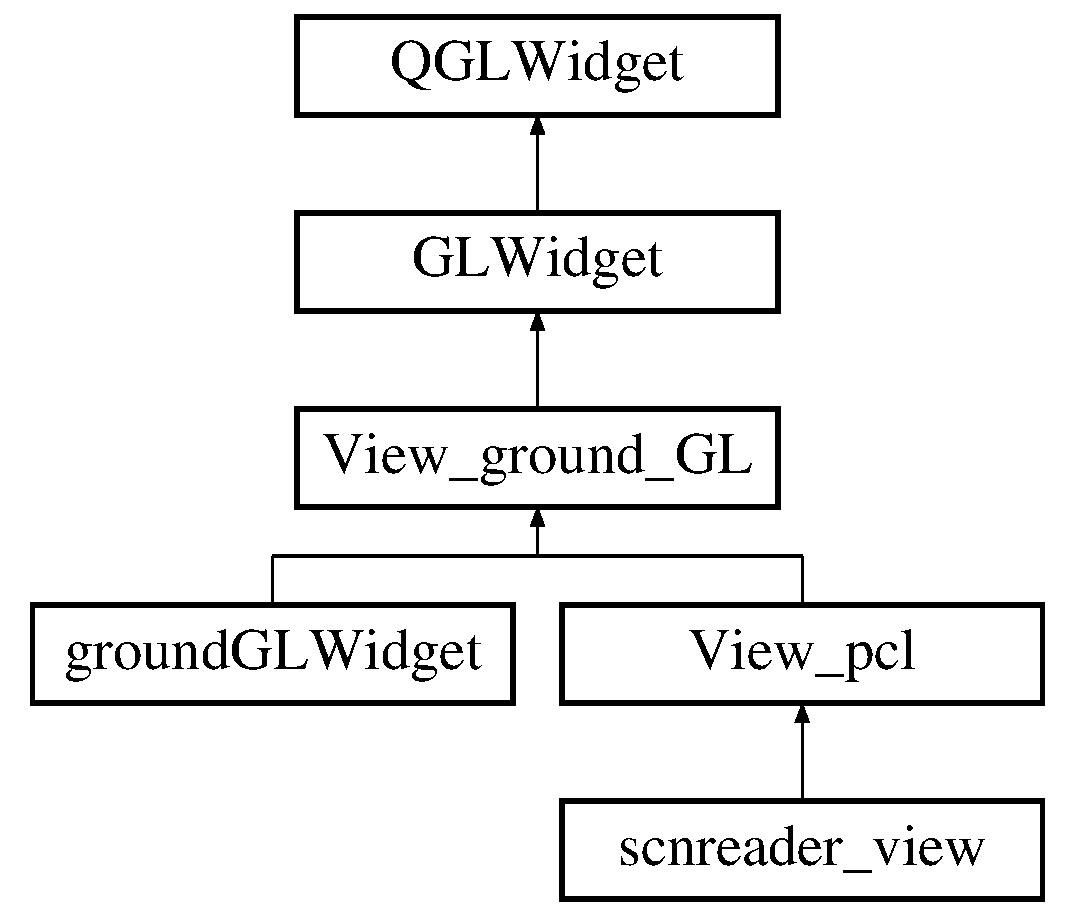
\includegraphics[height=5.000000cm]{classGLWidget}
\end{center}
\end{figure}
\subsection*{Public Slots}
\begin{DoxyCompactItemize}
\item 
\hypertarget{classGLWidget_af6539acfbeb3808ec22c23796631223a}{virtual void {\bfseries time\-Out\-Slot} ()}\label{classGLWidget_af6539acfbeb3808ec22c23796631223a}

\end{DoxyCompactItemize}
\subsection*{Public Member Functions}
\begin{DoxyCompactItemize}
\item 
\hypertarget{classGLWidget_a239ba4cdaf17dd41c6458db90e153211}{{\bfseries G\-L\-Widget} (int frames\-Per\-Second=0, Q\-Widget $\ast$parent=0, char $\ast$name=0)}\label{classGLWidget_a239ba4cdaf17dd41c6458db90e153211}

\item 
\hypertarget{classGLWidget_a8dcea17ae790967200534864412e4812}{virtual void {\bfseries initialize\-G\-L} ()=0}\label{classGLWidget_a8dcea17ae790967200534864412e4812}

\item 
\hypertarget{classGLWidget_a168f325cd90d1d5f6e2d27e1017d337f}{virtual void {\bfseries resize\-G\-L} (int width, int height)=0}\label{classGLWidget_a168f325cd90d1d5f6e2d27e1017d337f}

\item 
\hypertarget{classGLWidget_a3cad0d8f57b6253cf265d258ca327010}{virtual void {\bfseries paint\-G\-L} ()=0}\label{classGLWidget_a3cad0d8f57b6253cf265d258ca327010}

\item 
\hypertarget{classGLWidget_acee9343100914094424c31afd2603335}{bool {\bfseries full\-Window} ()}\label{classGLWidget_acee9343100914094424c31afd2603335}

\end{DoxyCompactItemize}
\subsection*{Protected Attributes}
\begin{DoxyCompactItemize}
\item 
\hypertarget{classGLWidget_ad13ccbe42c40518e3a347f21f247c51a}{bool {\bfseries b\-\_\-\-Fullscreen}}\label{classGLWidget_ad13ccbe42c40518e3a347f21f247c51a}

\end{DoxyCompactItemize}


The documentation for this class was generated from the following files\-:\begin{DoxyCompactItemize}
\item 
modules/open\-G\-L/ground/model/G\-L\-Widget.\-h\item 
modules/open\-G\-L/ground/model/G\-L\-Widget.\-cpp\end{DoxyCompactItemize}

\hypertarget{classgroundGLWidget}{\section{ground\-G\-L\-Widget Class Reference}
\label{classgroundGLWidget}\index{ground\-G\-L\-Widget@{ground\-G\-L\-Widget}}
}


The \hyperlink{classgroundGLWidget}{ground\-G\-L\-Widget} class This class grouped the main function open\-G\-L. Each function is already implemented and allows easy use of open\-G\-L . For more functionalities, You could overloading each function into a new class.  




{\ttfamily \#include $<$groundglwidget.\-h$>$}

Inheritance diagram for ground\-G\-L\-Widget\-:\begin{figure}[H]
\begin{center}
\leavevmode
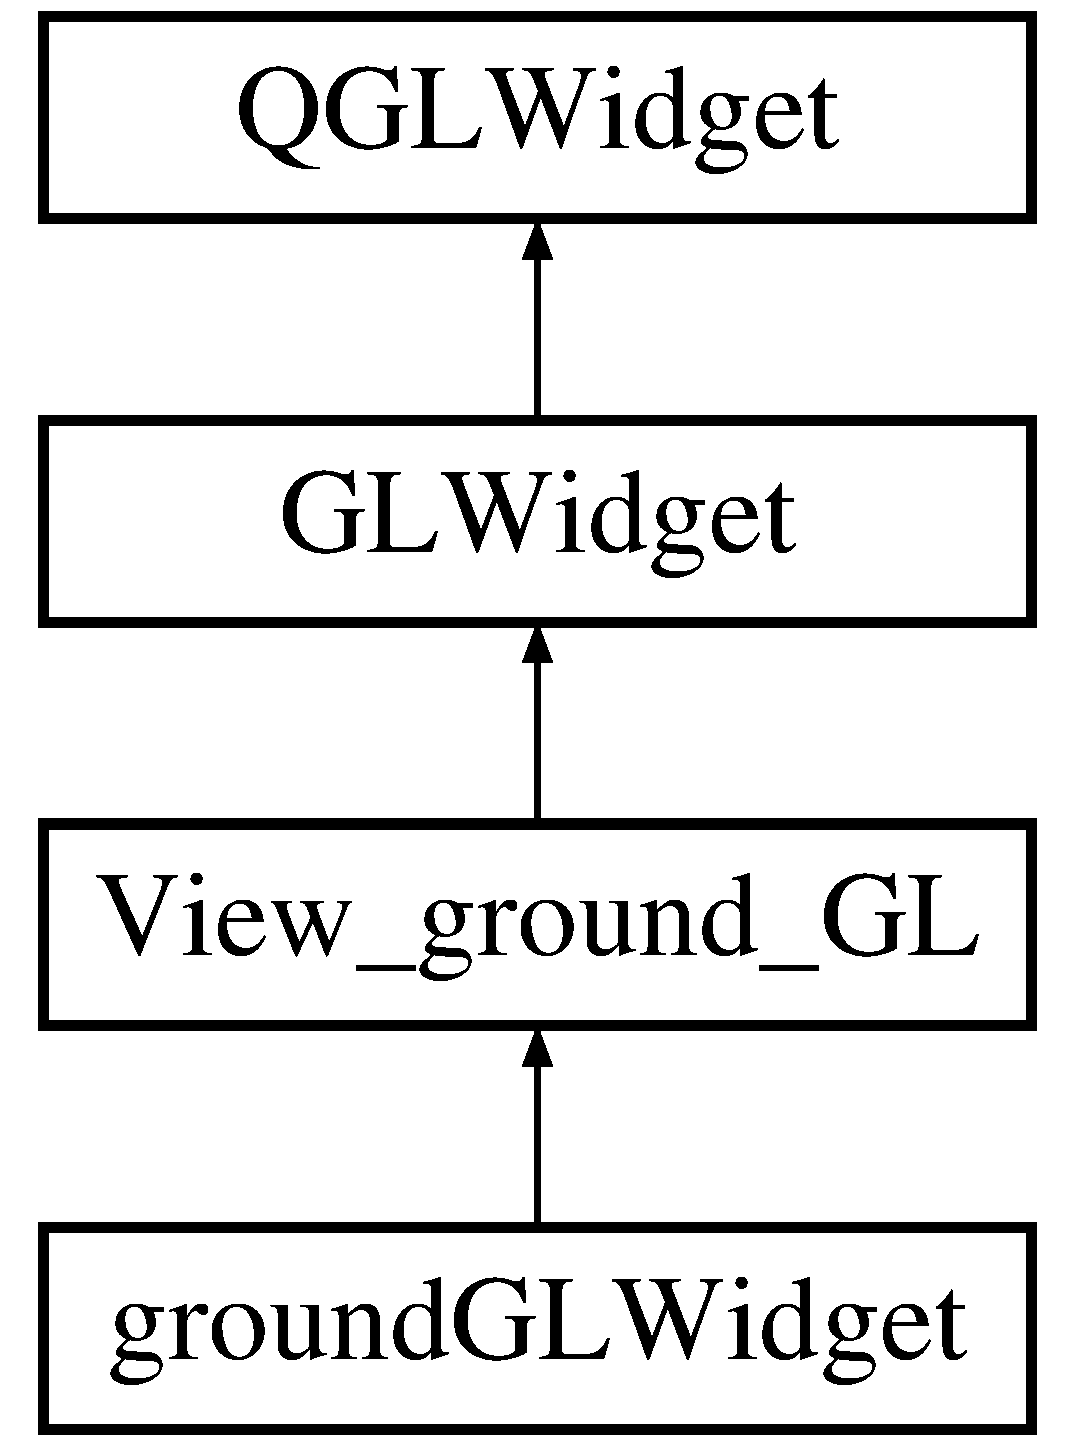
\includegraphics[height=4.000000cm]{classgroundGLWidget}
\end{center}
\end{figure}
\subsection*{Public Member Functions}
\begin{DoxyCompactItemize}
\item 
\hyperlink{classgroundGLWidget_ace71a5495d43d9a7c44d309d99fa8588}{ground\-G\-L\-Widget} (Q\-Widget $\ast$parent=0)
\begin{DoxyCompactList}\small\item\em \hyperlink{classgroundGLWidget}{ground\-G\-L\-Widget} constructor \end{DoxyCompactList}\item 
void \hyperlink{classgroundGLWidget_a4851c8cda48540aa8dcbc587977b3c29}{resize\-G\-L} (int width, int height)
\begin{DoxyCompactList}\small\item\em resize\-G\-L Resize open\-G\-L window. This function determines the most addaptees visualization parameters to the size of the open\-G\-L windows \end{DoxyCompactList}\item 
\hypertarget{classgroundGLWidget_af0df613d7935ac62d02c60d279b169a1}{void \hyperlink{classgroundGLWidget_af0df613d7935ac62d02c60d279b169a1}{initialize\-G\-L} ()}\label{classgroundGLWidget_af0df613d7935ac62d02c60d279b169a1}

\begin{DoxyCompactList}\small\item\em initialize\-G\-L it initialize all required parameters to open\-G\-L . \end{DoxyCompactList}\item 
\hypertarget{classgroundGLWidget_a5ff9c3eb738112242c4151dae2e5b467}{void \hyperlink{classgroundGLWidget_a5ff9c3eb738112242c4151dae2e5b467}{paint\-G\-L} ()}\label{classgroundGLWidget_a5ff9c3eb738112242c4151dae2e5b467}

\begin{DoxyCompactList}\small\item\em paint\-G\-L draw function of open\-G\-L \end{DoxyCompactList}\item 
\hypertarget{classgroundGLWidget_a833bec87ec0d0769e6b33c97f744d2ec}{virtual void {\bfseries key\-Press\-Event} (Q\-Key\-Event $\ast$key\-Event)}\label{classgroundGLWidget_a833bec87ec0d0769e6b33c97f744d2ec}

\item 
\hypertarget{classgroundGLWidget_a0d3f814a70a30fa15ecb746ba4ddb6f5}{virtual void {\bfseries mouse\-Press\-Event} (Q\-Mouse\-Event $\ast$event)}\label{classgroundGLWidget_a0d3f814a70a30fa15ecb746ba4ddb6f5}

\item 
\hypertarget{classgroundGLWidget_ad29a1b7d03ca35d7d07c205aa56e3bdc}{virtual void {\bfseries mouse\-Release\-Event} (Q\-Mouse\-Event $\ast$event)}\label{classgroundGLWidget_ad29a1b7d03ca35d7d07c205aa56e3bdc}

\item 
\hypertarget{classgroundGLWidget_ad68155f7ac7a2c53f24627aaa870082e}{virtual void {\bfseries mouse\-Move\-Event} (Q\-Mouse\-Event $\ast$event)}\label{classgroundGLWidget_ad68155f7ac7a2c53f24627aaa870082e}

\end{DoxyCompactItemize}
\subsection*{Additional Inherited Members}


\subsection{Detailed Description}
The \hyperlink{classgroundGLWidget}{ground\-G\-L\-Widget} class This class grouped the main function open\-G\-L. Each function is already implemented and allows easy use of open\-G\-L . For more functionalities, You could overloading each function into a new class. 

\subsection{Constructor \& Destructor Documentation}
\hypertarget{classgroundGLWidget_ace71a5495d43d9a7c44d309d99fa8588}{\index{ground\-G\-L\-Widget@{ground\-G\-L\-Widget}!ground\-G\-L\-Widget@{ground\-G\-L\-Widget}}
\index{ground\-G\-L\-Widget@{ground\-G\-L\-Widget}!groundGLWidget@{ground\-G\-L\-Widget}}
\subsubsection[{ground\-G\-L\-Widget}]{\setlength{\rightskip}{0pt plus 5cm}ground\-G\-L\-Widget\-::ground\-G\-L\-Widget (
\begin{DoxyParamCaption}
\item[{Q\-Widget $\ast$}]{parent = {\ttfamily 0}}
\end{DoxyParamCaption}
)}}\label{classgroundGLWidget_ace71a5495d43d9a7c44d309d99fa8588}


\hyperlink{classgroundGLWidget}{ground\-G\-L\-Widget} constructor 


\begin{DoxyParams}{Parameters}
{\em parent} & \\
\hline
\end{DoxyParams}


\subsection{Member Function Documentation}
\hypertarget{classgroundGLWidget_a4851c8cda48540aa8dcbc587977b3c29}{\index{ground\-G\-L\-Widget@{ground\-G\-L\-Widget}!resize\-G\-L@{resize\-G\-L}}
\index{resize\-G\-L@{resize\-G\-L}!groundGLWidget@{ground\-G\-L\-Widget}}
\subsubsection[{resize\-G\-L}]{\setlength{\rightskip}{0pt plus 5cm}void ground\-G\-L\-Widget\-::resize\-G\-L (
\begin{DoxyParamCaption}
\item[{int}]{width, }
\item[{int}]{height}
\end{DoxyParamCaption}
)\hspace{0.3cm}{\ttfamily [virtual]}}}\label{classgroundGLWidget_a4851c8cda48540aa8dcbc587977b3c29}


resize\-G\-L Resize open\-G\-L window. This function determines the most addaptees visualization parameters to the size of the open\-G\-L windows 


\begin{DoxyParams}{Parameters}
{\em width} & width of windows in pixel \\
\hline
{\em height} & height of windows in pixel \\
\hline
\end{DoxyParams}


Implements \hyperlink{classGLWidget}{G\-L\-Widget}.



The documentation for this class was generated from the following files\-:\begin{DoxyCompactItemize}
\item 
modules/open\-G\-L/ground/\hyperlink{groundglwidget_8h}{groundglwidget.\-h}\item 
modules/open\-G\-L/ground/groundglwidget.\-cpp\end{DoxyCompactItemize}

\hypertarget{classLesTextures}{\section{Les\-Textures Class Reference}
\label{classLesTextures}\index{Les\-Textures@{Les\-Textures}}
}


{\ttfamily \#include $<$Les\-Textures.\-h$>$}

\subsection*{Public Member Functions}
\begin{DoxyCompactItemize}
\item 
\hyperlink{classLesTextures_ae10396e044c7aa1749467834e5db8511}{Les\-Textures} ()
\item 
\hypertarget{classLesTextures_a3429b8579023d848474c9b109cc83a29}{{\bfseries Les\-Textures} (const \hyperlink{classLesTextures}{Les\-Textures} \&orig)}\label{classLesTextures_a3429b8579023d848474c9b109cc83a29}

\item 
void \hyperlink{classLesTextures_af3f3b9cde73b9f07abc980c62d26f0b0}{add} (\hyperlink{classTexture}{Texture} $\ast$t)
\item 
void \hyperlink{classLesTextures_aa55360dbfbc2d2799e0fdd4ba0167450}{add} (Q\-String adresse, std\-::string nom, G\-Luint id)
\item 
void \hyperlink{classLesTextures_a0132a8028f2fc67160268f80c4c79d63}{add} (Q\-String adresse, std\-::string nom)
\begin{DoxyCompactList}\small\item\em add ajoute un texture avec son nom l'identifiant \end{DoxyCompactList}\item 
void \hyperlink{classLesTextures_a02432688ee521372e71b7d0b32cd2b02}{affiche\-Texture} (std\-::string nom) const 
\item 
\hyperlink{classTexture}{Texture} $\ast$ \hyperlink{classLesTextures_ad41096dedc9ab42f0d9d4e93bc4a0794}{get\-Texture} (std\-::string nom)
\end{DoxyCompactItemize}


\subsection{Detailed Description}
\begin{DoxyAuthor}{Author}
P\-O\-N\-C\-I\-A\-N\-O Jean-\/\-Jacques et P\-R\-U\-D\-H\-O\-M\-M\-E Claire 
\end{DoxyAuthor}
\begin{DoxyDate}{Date}
13/03/2014
\end{DoxyDate}
Cette oeuvre, création, code, site ou texte est sous licence Creative Commons Attribution -\/ Pas d’\-Utilisation Commerciale -\/ Partage dans les Mêmes Conditions 4.\-0 International. Pour accéder à une copie de cette licence, merci de vous rendre à l'adresse suivante \href{http://creativecommons.org/licenses/by-nc-sa/4.0/deed.fr}{\tt http\-://creativecommons.\-org/licenses/by-\/nc-\/sa/4.\-0/deed.\-fr} ou envoyez un courrier à Creative Commons, 444 Castro Street, Suite 900, Mountain View, California, 94041, U\-S\-A. Copyright 2014

Contact\-: \href{mailto:ponciano.jeanjacques@gmail.com}{\tt ponciano.\-jeanjacques@gmail.\-com} 

\subsection{Constructor \& Destructor Documentation}
\hypertarget{classLesTextures_ae10396e044c7aa1749467834e5db8511}{\index{Les\-Textures@{Les\-Textures}!Les\-Textures@{Les\-Textures}}
\index{Les\-Textures@{Les\-Textures}!LesTextures@{Les\-Textures}}
\subsubsection[{Les\-Textures}]{\setlength{\rightskip}{0pt plus 5cm}Les\-Textures\-::\-Les\-Textures (
\begin{DoxyParamCaption}
{}
\end{DoxyParamCaption}
)}}\label{classLesTextures_ae10396e044c7aa1749467834e5db8511}
Constructeur 

\subsection{Member Function Documentation}
\hypertarget{classLesTextures_af3f3b9cde73b9f07abc980c62d26f0b0}{\index{Les\-Textures@{Les\-Textures}!add@{add}}
\index{add@{add}!LesTextures@{Les\-Textures}}
\subsubsection[{add}]{\setlength{\rightskip}{0pt plus 5cm}void Les\-Textures\-::add (
\begin{DoxyParamCaption}
\item[{{\bf Texture} $\ast$}]{t}
\end{DoxyParamCaption}
)}}\label{classLesTextures_af3f3b9cde73b9f07abc980c62d26f0b0}
Ajoute une texture 
\begin{DoxyParams}{Parameters}
{\em t} & texture à ajouter \\
\hline
\end{DoxyParams}
\hypertarget{classLesTextures_aa55360dbfbc2d2799e0fdd4ba0167450}{\index{Les\-Textures@{Les\-Textures}!add@{add}}
\index{add@{add}!LesTextures@{Les\-Textures}}
\subsubsection[{add}]{\setlength{\rightskip}{0pt plus 5cm}void Les\-Textures\-::add (
\begin{DoxyParamCaption}
\item[{Q\-String}]{adresse, }
\item[{std\-::string}]{nom, }
\item[{G\-Luint}]{id}
\end{DoxyParamCaption}
)}}\label{classLesTextures_aa55360dbfbc2d2799e0fdd4ba0167450}
Ajoute et crée une texture 
\begin{DoxyParams}{Parameters}
{\em adresse} & adresse de l'image \\
\hline
{\em nom} & nom de la texture \\
\hline
\end{DoxyParams}
\hypertarget{classLesTextures_a0132a8028f2fc67160268f80c4c79d63}{\index{Les\-Textures@{Les\-Textures}!add@{add}}
\index{add@{add}!LesTextures@{Les\-Textures}}
\subsubsection[{add}]{\setlength{\rightskip}{0pt plus 5cm}void Les\-Textures\-::add (
\begin{DoxyParamCaption}
\item[{Q\-String}]{adresse, }
\item[{std\-::string}]{nom}
\end{DoxyParamCaption}
)}}\label{classLesTextures_a0132a8028f2fc67160268f80c4c79d63}


add ajoute un texture avec son nom l'identifiant 


\begin{DoxyParams}{Parameters}
{\em adresse} & adresse ou charger la texture \\
\hline
{\em nom} & identifiant de la texture \\
\hline
\end{DoxyParams}
\hypertarget{classLesTextures_a02432688ee521372e71b7d0b32cd2b02}{\index{Les\-Textures@{Les\-Textures}!affiche\-Texture@{affiche\-Texture}}
\index{affiche\-Texture@{affiche\-Texture}!LesTextures@{Les\-Textures}}
\subsubsection[{affiche\-Texture}]{\setlength{\rightskip}{0pt plus 5cm}void Les\-Textures\-::affiche\-Texture (
\begin{DoxyParamCaption}
\item[{std\-::string}]{nom}
\end{DoxyParamCaption}
) const}}\label{classLesTextures_a02432688ee521372e71b7d0b32cd2b02}
Affiche/applique la texture 
\begin{DoxyParams}{Parameters}
{\em nom} & nom de la texture à affiche/applique \\
\hline
\end{DoxyParams}
\hypertarget{classLesTextures_ad41096dedc9ab42f0d9d4e93bc4a0794}{\index{Les\-Textures@{Les\-Textures}!get\-Texture@{get\-Texture}}
\index{get\-Texture@{get\-Texture}!LesTextures@{Les\-Textures}}
\subsubsection[{get\-Texture}]{\setlength{\rightskip}{0pt plus 5cm}{\bf Texture} $\ast$ Les\-Textures\-::get\-Texture (
\begin{DoxyParamCaption}
\item[{std\-::string}]{nom}
\end{DoxyParamCaption}
)}}\label{classLesTextures_ad41096dedc9ab42f0d9d4e93bc4a0794}
Récupère la texture 
\begin{DoxyParams}{Parameters}
{\em nom} & nom de la texture à récupérer \\
\hline
\end{DoxyParams}
\begin{DoxyReturn}{Returns}
texture portant le nom donné 
\end{DoxyReturn}


The documentation for this class was generated from the following files\-:\begin{DoxyCompactItemize}
\item 
modules/open\-G\-L/ground/model/Les\-Textures.\-h\item 
modules/open\-G\-L/ground/model/Les\-Textures.\-cpp\end{DoxyCompactItemize}

\hypertarget{classMagicfish}{\section{Magicfish Class Reference}
\label{classMagicfish}\index{Magicfish@{Magicfish}}
}
\subsection*{Public Member Functions}
\begin{DoxyCompactItemize}
\item 
\hypertarget{classMagicfish_a4d4ad0aa6941821a56d1a015671b1c65}{\hyperlink{classMagicfish_a4d4ad0aa6941821a56d1a015671b1c65}{Magicfish} ()}\label{classMagicfish_a4d4ad0aa6941821a56d1a015671b1c65}

\begin{DoxyCompactList}\small\item\em \hyperlink{classMagicfish}{Magicfish} constructeur. \end{DoxyCompactList}\item 
\hypertarget{classMagicfish_a90ff3fb674ad6910912e93e4356581ad}{Q\-Image {\bfseries processing} (Q\-Image qi)}\label{classMagicfish_a90ff3fb674ad6910912e93e4356581ad}

\item 
Q\-Image \hyperlink{classMagicfish_aca3e8f97bfb995fbcd504cc79369cec9}{Modification} (int intensite, int brillance, float seuil, int x, int y, Q\-Image im)
\begin{DoxyCompactList}\small\item\em Modification. \end{DoxyCompactList}\item 
\hypertarget{classMagicfish_a041b2e4933fac43533bf358f6eadb1af}{void {\bfseries initialization} (std\-::string input)}\label{classMagicfish_a041b2e4933fac43533bf358f6eadb1af}

\item 
\hypertarget{classMagicfish_af5fc5198309c895a1961954cc4eff4c9}{Q\-Image {\bfseries difference} (Q\-Image I, Q\-Image I2, int threshold, int closing\-\_\-size, int last\-\_\-closing\-\_\-size, int opening\-\_\-size)}\label{classMagicfish_af5fc5198309c895a1961954cc4eff4c9}

\item 
\hypertarget{classMagicfish_ac5e098b5e72687bfade751eaf4a03a55}{Q\-Image {\bfseries get\-Fish} (Q\-Image im\-Or, Q\-Image im\-F1, Q\-Image im\-F2, Q\-Image im\-F3, int threshold, int closing\-\_\-size, int last\-\_\-closing\-\_\-size, int opening\-\_\-size)}\label{classMagicfish_ac5e098b5e72687bfade751eaf4a03a55}

\item 
\hypertarget{classMagicfish_a00ceb1c3e41cbae30ea3127e40742867}{void {\bfseries video} (std\-::string video\-Name, std\-::string path\-Output)}\label{classMagicfish_a00ceb1c3e41cbae30ea3127e40742867}

\item 
\hypertarget{classMagicfish_a622cabef45a1b89a1dc0d721c1f6ce9c}{void {\bfseries whrite\-Video} (std\-::string input, std\-::string output)}\label{classMagicfish_a622cabef45a1b89a1dc0d721c1f6ce9c}

\item 
\hypertarget{classMagicfish_aab353650bd7bedd593a7101770ee102d}{void {\bfseries whrite\-Video\-Def\-Background} (std\-::string input, std\-::string output)}\label{classMagicfish_aab353650bd7bedd593a7101770ee102d}

\item 
\hypertarget{classMagicfish_ab6701d65cbd335d58c7436991230ae35}{Q\-Image {\bfseries Recup\-Image} (cv\-::\-Mat matrice)}\label{classMagicfish_ab6701d65cbd335d58c7436991230ae35}

\item 
\hypertarget{classMagicfish_aacf4643de36b5ca777439b2682eb73f3}{Q\-Image {\bfseries get\-Background} (int indice\-Background)}\label{classMagicfish_aacf4643de36b5ca777439b2682eb73f3}

\item 
\hypertarget{classMagicfish_aa5d1d72ed90f8d0585852321302dafa9}{int {\bfseries get\-Threshold} ()}\label{classMagicfish_aa5d1d72ed90f8d0585852321302dafa9}

\item 
\hypertarget{classMagicfish_aac4e17cd338db300bb71f335ce8ed11c}{int {\bfseries getclosing\-\_\-size} ()}\label{classMagicfish_aac4e17cd338db300bb71f335ce8ed11c}

\item 
\hypertarget{classMagicfish_aaeb5e0a3f4cc9f0b5965f6d474e1a2c0}{int {\bfseries get\-Last\-\_\-closing\-\_\-size} ()}\label{classMagicfish_aaeb5e0a3f4cc9f0b5965f6d474e1a2c0}

\item 
\hypertarget{classMagicfish_a0dbc287a6da6da9f46b3bf82f59cfd07}{int {\bfseries get\-Opening\-\_\-size} ()}\label{classMagicfish_a0dbc287a6da6da9f46b3bf82f59cfd07}

\item 
\hypertarget{classMagicfish_aa50681ec40c30bfe411904018672b799}{void {\bfseries set\-Background} (int indice\-Background, Q\-Image qi)}\label{classMagicfish_aa50681ec40c30bfe411904018672b799}

\item 
\hypertarget{classMagicfish_a1bd3820e37d0d37ab1464530fa55286d}{void {\bfseries set\-Threshold} (int t)}\label{classMagicfish_a1bd3820e37d0d37ab1464530fa55286d}

\item 
\hypertarget{classMagicfish_adabdc34e3b24819bdcbaa8982feab371}{void {\bfseries setclosing\-\_\-size} (int c)}\label{classMagicfish_adabdc34e3b24819bdcbaa8982feab371}

\item 
\hypertarget{classMagicfish_ae1bc443abd6c1ca3b0baa41b8839c7cd}{void {\bfseries set\-Last\-\_\-closing\-\_\-size} (int c)}\label{classMagicfish_ae1bc443abd6c1ca3b0baa41b8839c7cd}

\item 
\hypertarget{classMagicfish_a60cac7f487621409afdaa309426a9cce}{void {\bfseries set\-Opening\-\_\-size} (int o)}\label{classMagicfish_a60cac7f487621409afdaa309426a9cce}

\end{DoxyCompactItemize}
\subsection*{Static Public Member Functions}
\begin{DoxyCompactItemize}
\item 
\hypertarget{classMagicfish_aa5d0ccd0ad4828a556b75613b0ac3122}{static void {\bfseries init\-Donnees\-System} ()}\label{classMagicfish_aa5d0ccd0ad4828a556b75613b0ac3122}

\end{DoxyCompactItemize}
\subsection*{Public Attributes}
\begin{DoxyCompactItemize}
\item 
\hypertarget{classMagicfish_ac3bc610b1ec104bc97086fbaf9649b3e}{Q\-Image {\bfseries background1}}\label{classMagicfish_ac3bc610b1ec104bc97086fbaf9649b3e}

\item 
\hypertarget{classMagicfish_a80410c901593d0a34bd641d33d78d8d5}{Q\-Image {\bfseries background2}}\label{classMagicfish_a80410c901593d0a34bd641d33d78d8d5}

\item 
\hypertarget{classMagicfish_a62bff4cfa3b186f157f5782060281f4a}{Q\-Image {\bfseries background3}}\label{classMagicfish_a62bff4cfa3b186f157f5782060281f4a}

\item 
\hypertarget{classMagicfish_ac3e144f2565649a7174caad3d6ab6031}{int {\bfseries threshold}}\label{classMagicfish_ac3e144f2565649a7174caad3d6ab6031}

\item 
\hypertarget{classMagicfish_ab6679a7be2d662dffb72dccfa11aba59}{int {\bfseries closing\-\_\-size}}\label{classMagicfish_ab6679a7be2d662dffb72dccfa11aba59}

\item 
\hypertarget{classMagicfish_af9c1320b45a3a617f929268481c1c668}{int {\bfseries last\-\_\-closing\-\_\-size}}\label{classMagicfish_af9c1320b45a3a617f929268481c1c668}

\item 
\hypertarget{classMagicfish_aba2b77f24cc97794425992b409ff6bcf}{int {\bfseries opening\-\_\-size}}\label{classMagicfish_aba2b77f24cc97794425992b409ff6bcf}

\item 
\hypertarget{classMagicfish_a2d79353c6352addba1055a3fd76e8748}{int {\bfseries intensite}}\label{classMagicfish_a2d79353c6352addba1055a3fd76e8748}

\item 
\hypertarget{classMagicfish_a72ab822bc8134e9456426a88ffeb3f42}{int {\bfseries brillance}}\label{classMagicfish_a72ab822bc8134e9456426a88ffeb3f42}

\item 
\hypertarget{classMagicfish_a8d18431136e6b69a3a3c4e717c080513}{float {\bfseries seuil}}\label{classMagicfish_a8d18431136e6b69a3a3c4e717c080513}

\item 
\hypertarget{classMagicfish_ab3bcb471d2afd306f06e6203b48aa963}{std\-::string {\bfseries inputfilename}}\label{classMagicfish_ab3bcb471d2afd306f06e6203b48aa963}

\item 
\hypertarget{classMagicfish_a072b7ab98da01837ea024466793200d7}{int {\bfseries x}}\label{classMagicfish_a072b7ab98da01837ea024466793200d7}

\item 
\hypertarget{classMagicfish_ac39de8728f6243284cb7230e9ff7fd69}{int {\bfseries y}}\label{classMagicfish_ac39de8728f6243284cb7230e9ff7fd69}

\end{DoxyCompactItemize}


\subsection{Member Function Documentation}
\hypertarget{classMagicfish_aca3e8f97bfb995fbcd504cc79369cec9}{\index{Magicfish@{Magicfish}!Modification@{Modification}}
\index{Modification@{Modification}!Magicfish@{Magicfish}}
\subsubsection[{Modification}]{\setlength{\rightskip}{0pt plus 5cm}Q\-Image Magicfish\-::\-Modification (
\begin{DoxyParamCaption}
\item[{int}]{intensite, }
\item[{int}]{brillance, }
\item[{float}]{seuil, }
\item[{int}]{x, }
\item[{int}]{y, }
\item[{Q\-Image}]{im}
\end{DoxyParamCaption}
)}}\label{classMagicfish_aca3e8f97bfb995fbcd504cc79369cec9}


Modification. 


\begin{DoxyParams}{Parameters}
{\em intensite} & coefficient d'intensité \\
\hline
{\em brillance} & coefficient de brillance \\
\hline
{\em seuil} & de tolérance de la teinte/couleur \\
\hline
{\em i} & coordonnée du pixel servant de référence \\
\hline
{\em j} & coordonnée du pixel servant de référence \\
\hline
\end{DoxyParams}
\begin{DoxyReturn}{Returns}
l'image résultante de la modification d'intensité(valeur) et de brillance(saturation) 
\end{DoxyReturn}


The documentation for this class was generated from the following files\-:\begin{DoxyCompactItemize}
\item 
modules/open\-C\-V/magicfish.\-h\item 
modules/open\-C\-V/magicfish.\-cpp\end{DoxyCompactItemize}

\hypertarget{classMainWindow}{\section{Main\-Window Class Reference}
\label{classMainWindow}\index{Main\-Window@{Main\-Window}}
}
Inheritance diagram for Main\-Window\-:\begin{figure}[H]
\begin{center}
\leavevmode
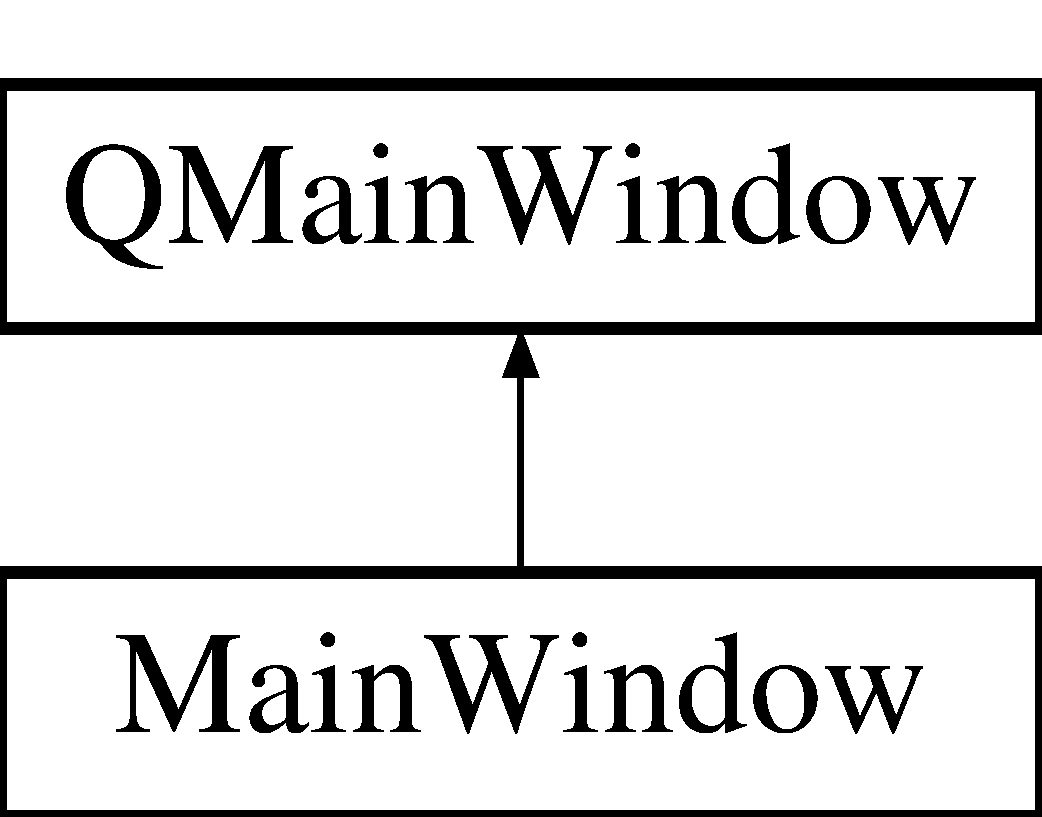
\includegraphics[height=2.000000cm]{classMainWindow}
\end{center}
\end{figure}
\subsection*{Public Slots}
\begin{DoxyCompactItemize}
\item 
\hypertarget{classMainWindow_a77557e32fb4ed3530daf2f6225c877db}{void {\bfseries clear} ()}\label{classMainWindow_a77557e32fb4ed3530daf2f6225c877db}

\item 
\hypertarget{classMainWindow_ad6bc77c2417da2a3728dd589c434dc6e}{void {\bfseries extract} ()}\label{classMainWindow_ad6bc77c2417da2a3728dd589c434dc6e}

\item 
\hypertarget{classMainWindow_ac47089e2ddbd6348bcd309f861da3a7d}{void {\bfseries planar\-Seg} ()}\label{classMainWindow_ac47089e2ddbd6348bcd309f861da3a7d}

\item 
\hypertarget{classMainWindow_a233bee15277ba8e4eebbb121bd547839}{void {\bfseries load\-From\-File} ()}\label{classMainWindow_a233bee15277ba8e4eebbb121bd547839}

\item 
\hypertarget{classMainWindow_a3052f4f925c5a0e4f8f6b7148e87ac01}{void {\bfseries load\-From\-S\-C\-N} ()}\label{classMainWindow_a3052f4f925c5a0e4f8f6b7148e87ac01}

\item 
\hypertarget{classMainWindow_ab89166f5ea7d7c22d475a83451819b5d}{void {\bfseries load\-Cloud\-From\-T\-X\-T} ()}\label{classMainWindow_ab89166f5ea7d7c22d475a83451819b5d}

\item 
\hypertarget{classMainWindow_a519b958c8619d8f7b3d97af8c70e70bb}{void {\bfseries save\-From\-File} ()}\label{classMainWindow_a519b958c8619d8f7b3d97af8c70e70bb}

\item 
\hypertarget{classMainWindow_aa05ba856ca3532f1c0f99d2bb74e9fb5}{void {\bfseries save\-From\-File\-T\-X\-T} ()}\label{classMainWindow_aa05ba856ca3532f1c0f99d2bb74e9fb5}

\end{DoxyCompactItemize}
\subsection*{Public Member Functions}
\begin{DoxyCompactItemize}
\item 
\hypertarget{classMainWindow_a8b244be8b7b7db1b08de2a2acb9409db}{{\bfseries Main\-Window} (Q\-Widget $\ast$parent=0)}\label{classMainWindow_a8b244be8b7b7db1b08de2a2acb9409db}

\item 
\hypertarget{classMainWindow_ab85c711e421fb0f0dfec5e4e68cbfa51}{virtual void {\bfseries key\-Press\-Event} (Q\-Key\-Event $\ast$key\-Event)}\label{classMainWindow_ab85c711e421fb0f0dfec5e4e68cbfa51}

\item 
\hypertarget{classMainWindow_a2b5463ae209a03d1680b39c950dac8be}{virtual void {\bfseries mouse\-Press\-Event} (Q\-Mouse\-Event $\ast$event)}\label{classMainWindow_a2b5463ae209a03d1680b39c950dac8be}

\item 
\hypertarget{classMainWindow_a32bbb036a55856e49c31a5348f937b53}{virtual void {\bfseries mouse\-Release\-Event} (Q\-Mouse\-Event $\ast$event)}\label{classMainWindow_a32bbb036a55856e49c31a5348f937b53}

\item 
\hypertarget{classMainWindow_a2cf42454562815dd44c716e78d515697}{virtual void {\bfseries mouse\-Move\-Event} (Q\-Mouse\-Event $\ast$event)}\label{classMainWindow_a2cf42454562815dd44c716e78d515697}

\end{DoxyCompactItemize}


The documentation for this class was generated from the following files\-:\begin{DoxyCompactItemize}
\item 
mainwindow.\-h\item 
mainwindow.\-cpp\end{DoxyCompactItemize}

\hypertarget{classMateriel}{\section{Materiel Class Reference}
\label{classMateriel}\index{Materiel@{Materiel}}
}


{\ttfamily \#include $<$Materiel.\-h$>$}

\subsection*{Public Member Functions}
\begin{DoxyCompactItemize}
\item 
\hyperlink{classMateriel_a0ddcbd4ce36253c1a698512571c0e070}{Materiel} ()
\item 
\hypertarget{classMateriel_ad95cee4ed27a06addace4e4c8ed2c245}{{\bfseries Materiel} (const \hyperlink{classMateriel}{Materiel} \&orig)}\label{classMateriel_ad95cee4ed27a06addace4e4c8ed2c245}

\item 
void \hyperlink{classMateriel_a66ca8d88c1512b56bf7b70ad22c34a66}{carrelage} ()
\item 
void \hyperlink{classMateriel_a6263dc9dce75300abbb35e735f765fe4}{emerald} ()
\item 
void \hyperlink{classMateriel_a77273ccb5baec1f6275f6c2f7b175046}{jade} ()
\item 
void \hyperlink{classMateriel_a85c785d70801ecc361b01057bba419f1}{obsidian} ()
\item 
void \hyperlink{classMateriel_abed4f19c5cfd912c9ac82e2b5a38e530}{pearl} ()
\item 
void \hyperlink{classMateriel_a52fb9aafbdc20f7e29ee1727e0a222fc}{ruby} ()
\item 
void \hyperlink{classMateriel_ae4e624b1b697a2b5badf44c49b0f7120}{turquoise} ()
\item 
void \hyperlink{classMateriel_a56f7b01a878aafdd7f0a000ce5766b64}{brass} ()
\item 
void \hyperlink{classMateriel_a366139f1dcc6eab79878c0db8a44da5a}{bronze} ()
\item 
void \hyperlink{classMateriel_a8c854cb036967c7834b9acbc0d349a0c}{chrome} ()
\item 
void \hyperlink{classMateriel_a8d5cc28a0a2dc40523efc8d939e13c8f}{copper} ()
\item 
void \hyperlink{classMateriel_ab314429173c74e86d0b29f55aa51ef6e}{gold} ()
\item 
void \hyperlink{classMateriel_a1d93d7785ff2819aeb199066271e0250}{silver} ()
\item 
void \hyperlink{classMateriel_a770d2cc0691ecea22b7c337821683a80}{blackplastic} ()
\item 
void \hyperlink{classMateriel_a5467964d2a54dac87623822625b2bbf0}{cyanplastic} ()
\item 
void \hyperlink{classMateriel_ad6d5df0bea8baa02f9dd40b55e17a3ce}{greenplastic} ()
\item 
void \hyperlink{classMateriel_ac6bf319b8e840dd9c3c10daf4c0ba079}{redplastic} ()
\item 
void \hyperlink{classMateriel_a92cc89e6c6048b4b7e0bc646006fd91c}{whiteplastic} ()
\item 
void \hyperlink{classMateriel_ac517aab56c14afaeb8475e08f86a7dad}{yellowplastic} ()
\item 
void \hyperlink{classMateriel_aa639a9a59b81aa81c3fa10e249260c4c}{blackrubber} ()
\item 
void \hyperlink{classMateriel_aea8f32c293e90d570ce440c8ecdd4745}{cyanrubber} ()
\item 
void \hyperlink{classMateriel_aaac30424a4c261bbabe99aa347988d81}{greenrubber} ()
\item 
void \hyperlink{classMateriel_ac730b39c254bc960a16f19e8f3722493}{redrubber} ()
\item 
void \hyperlink{classMateriel_a1c24aeb97eaa17553dfdb5933b2e64b6}{whiterubber} ()
\item 
void \hyperlink{classMateriel_ad528d3c44f5c517858d1dad0ecc7c834}{yellowrubber} ()
\item 
void \hyperlink{classMateriel_a0ad6369d4295b250ef2842b0b8f32668}{select\-Materiel} (int i)
\item 
void \hyperlink{classMateriel_a24cd089e317e0f1fa4e5f6ad9484d56c}{bois\-Claire} ()
\item 
void \hyperlink{classMateriel_a3f4e98359e1053457b5968f2d912de86}{peinture} ()
\item 
void \hyperlink{classMateriel_a8c0defabc9974f1801dfc82236d751ac}{Bois\-Fonce} ()
\item 
void \hyperlink{classMateriel_af61a650d8ff44c710f3258ab15bbf4f1}{vitre} ()
\item 
void \hyperlink{classMateriel_afa2f1d85a1980a94a3b58e1bdd7f81b3}{porcelaine} ()
\end{DoxyCompactItemize}


\subsection{Detailed Description}
\begin{DoxyAuthor}{Author}
P\-O\-N\-C\-I\-A\-N\-O Jean-\/\-Jacques et P\-R\-U\-D\-H\-O\-M\-M\-E Claire 
\end{DoxyAuthor}
\begin{DoxyDate}{Date}
13/03/2014
\end{DoxyDate}
Cette oeuvre, création, code, site ou texte est sous licence Creative Commons Attribution -\/ Pas d’\-Utilisation Commerciale -\/ Partage dans les Mêmes Conditions 4.\-0 International. Pour accéder à une copie de cette licence, merci de vous rendre à l'adresse suivante \href{http://creativecommons.org/licenses/by-nc-sa/4.0/deed.fr}{\tt http\-://creativecommons.\-org/licenses/by-\/nc-\/sa/4.\-0/deed.\-fr} ou envoyez un courrier à Creative Commons, 444 Castro Street, Suite 900, Mountain View, California, 94041, U\-S\-A. Copyright 2014

Contact\-: \href{mailto:ponciano.jeanjacques@gmail.com}{\tt ponciano.\-jeanjacques@gmail.\-com} 

\subsection{Constructor \& Destructor Documentation}
\hypertarget{classMateriel_a0ddcbd4ce36253c1a698512571c0e070}{\index{Materiel@{Materiel}!Materiel@{Materiel}}
\index{Materiel@{Materiel}!Materiel@{Materiel}}
\subsubsection[{Materiel}]{\setlength{\rightskip}{0pt plus 5cm}Materiel\-::\-Materiel (
\begin{DoxyParamCaption}
{}
\end{DoxyParamCaption}
)}}\label{classMateriel_a0ddcbd4ce36253c1a698512571c0e070}
Constructeur 

\subsection{Member Function Documentation}
\hypertarget{classMateriel_a770d2cc0691ecea22b7c337821683a80}{\index{Materiel@{Materiel}!blackplastic@{blackplastic}}
\index{blackplastic@{blackplastic}!Materiel@{Materiel}}
\subsubsection[{blackplastic}]{\setlength{\rightskip}{0pt plus 5cm}void Materiel\-::blackplastic (
\begin{DoxyParamCaption}
{}
\end{DoxyParamCaption}
)}}\label{classMateriel_a770d2cc0691ecea22b7c337821683a80}
Charge un matériau \hypertarget{classMateriel_aa639a9a59b81aa81c3fa10e249260c4c}{\index{Materiel@{Materiel}!blackrubber@{blackrubber}}
\index{blackrubber@{blackrubber}!Materiel@{Materiel}}
\subsubsection[{blackrubber}]{\setlength{\rightskip}{0pt plus 5cm}void Materiel\-::blackrubber (
\begin{DoxyParamCaption}
{}
\end{DoxyParamCaption}
)}}\label{classMateriel_aa639a9a59b81aa81c3fa10e249260c4c}
Charge un matériau \hypertarget{classMateriel_a24cd089e317e0f1fa4e5f6ad9484d56c}{\index{Materiel@{Materiel}!bois\-Claire@{bois\-Claire}}
\index{bois\-Claire@{bois\-Claire}!Materiel@{Materiel}}
\subsubsection[{bois\-Claire}]{\setlength{\rightskip}{0pt plus 5cm}void Materiel\-::bois\-Claire (
\begin{DoxyParamCaption}
{}
\end{DoxyParamCaption}
)}}\label{classMateriel_a24cd089e317e0f1fa4e5f6ad9484d56c}
Charge un matériau \hypertarget{classMateriel_a8c0defabc9974f1801dfc82236d751ac}{\index{Materiel@{Materiel}!Bois\-Fonce@{Bois\-Fonce}}
\index{Bois\-Fonce@{Bois\-Fonce}!Materiel@{Materiel}}
\subsubsection[{Bois\-Fonce}]{\setlength{\rightskip}{0pt plus 5cm}void Materiel\-::\-Bois\-Fonce (
\begin{DoxyParamCaption}
{}
\end{DoxyParamCaption}
)}}\label{classMateriel_a8c0defabc9974f1801dfc82236d751ac}
Charge un matériau \hypertarget{classMateriel_a56f7b01a878aafdd7f0a000ce5766b64}{\index{Materiel@{Materiel}!brass@{brass}}
\index{brass@{brass}!Materiel@{Materiel}}
\subsubsection[{brass}]{\setlength{\rightskip}{0pt plus 5cm}void Materiel\-::brass (
\begin{DoxyParamCaption}
{}
\end{DoxyParamCaption}
)}}\label{classMateriel_a56f7b01a878aafdd7f0a000ce5766b64}
Charge un matériau \hypertarget{classMateriel_a366139f1dcc6eab79878c0db8a44da5a}{\index{Materiel@{Materiel}!bronze@{bronze}}
\index{bronze@{bronze}!Materiel@{Materiel}}
\subsubsection[{bronze}]{\setlength{\rightskip}{0pt plus 5cm}void Materiel\-::bronze (
\begin{DoxyParamCaption}
{}
\end{DoxyParamCaption}
)}}\label{classMateriel_a366139f1dcc6eab79878c0db8a44da5a}
Charge un matériau \hypertarget{classMateriel_a66ca8d88c1512b56bf7b70ad22c34a66}{\index{Materiel@{Materiel}!carrelage@{carrelage}}
\index{carrelage@{carrelage}!Materiel@{Materiel}}
\subsubsection[{carrelage}]{\setlength{\rightskip}{0pt plus 5cm}void Materiel\-::carrelage (
\begin{DoxyParamCaption}
{}
\end{DoxyParamCaption}
)}}\label{classMateriel_a66ca8d88c1512b56bf7b70ad22c34a66}
Charge un matériau \hypertarget{classMateriel_a8c854cb036967c7834b9acbc0d349a0c}{\index{Materiel@{Materiel}!chrome@{chrome}}
\index{chrome@{chrome}!Materiel@{Materiel}}
\subsubsection[{chrome}]{\setlength{\rightskip}{0pt plus 5cm}void Materiel\-::chrome (
\begin{DoxyParamCaption}
{}
\end{DoxyParamCaption}
)}}\label{classMateriel_a8c854cb036967c7834b9acbc0d349a0c}
Charge un matériau \hypertarget{classMateriel_a8d5cc28a0a2dc40523efc8d939e13c8f}{\index{Materiel@{Materiel}!copper@{copper}}
\index{copper@{copper}!Materiel@{Materiel}}
\subsubsection[{copper}]{\setlength{\rightskip}{0pt plus 5cm}void Materiel\-::copper (
\begin{DoxyParamCaption}
{}
\end{DoxyParamCaption}
)}}\label{classMateriel_a8d5cc28a0a2dc40523efc8d939e13c8f}
Charge un matériau \hypertarget{classMateriel_a5467964d2a54dac87623822625b2bbf0}{\index{Materiel@{Materiel}!cyanplastic@{cyanplastic}}
\index{cyanplastic@{cyanplastic}!Materiel@{Materiel}}
\subsubsection[{cyanplastic}]{\setlength{\rightskip}{0pt plus 5cm}void Materiel\-::cyanplastic (
\begin{DoxyParamCaption}
{}
\end{DoxyParamCaption}
)}}\label{classMateriel_a5467964d2a54dac87623822625b2bbf0}
Charge un matériau \hypertarget{classMateriel_aea8f32c293e90d570ce440c8ecdd4745}{\index{Materiel@{Materiel}!cyanrubber@{cyanrubber}}
\index{cyanrubber@{cyanrubber}!Materiel@{Materiel}}
\subsubsection[{cyanrubber}]{\setlength{\rightskip}{0pt plus 5cm}void Materiel\-::cyanrubber (
\begin{DoxyParamCaption}
{}
\end{DoxyParamCaption}
)}}\label{classMateriel_aea8f32c293e90d570ce440c8ecdd4745}
Charge un matériau \hypertarget{classMateriel_a6263dc9dce75300abbb35e735f765fe4}{\index{Materiel@{Materiel}!emerald@{emerald}}
\index{emerald@{emerald}!Materiel@{Materiel}}
\subsubsection[{emerald}]{\setlength{\rightskip}{0pt plus 5cm}void Materiel\-::emerald (
\begin{DoxyParamCaption}
{}
\end{DoxyParamCaption}
)}}\label{classMateriel_a6263dc9dce75300abbb35e735f765fe4}
Charge un matériau \hypertarget{classMateriel_ab314429173c74e86d0b29f55aa51ef6e}{\index{Materiel@{Materiel}!gold@{gold}}
\index{gold@{gold}!Materiel@{Materiel}}
\subsubsection[{gold}]{\setlength{\rightskip}{0pt plus 5cm}void Materiel\-::gold (
\begin{DoxyParamCaption}
{}
\end{DoxyParamCaption}
)}}\label{classMateriel_ab314429173c74e86d0b29f55aa51ef6e}
Charge un matériau \hypertarget{classMateriel_ad6d5df0bea8baa02f9dd40b55e17a3ce}{\index{Materiel@{Materiel}!greenplastic@{greenplastic}}
\index{greenplastic@{greenplastic}!Materiel@{Materiel}}
\subsubsection[{greenplastic}]{\setlength{\rightskip}{0pt plus 5cm}void Materiel\-::greenplastic (
\begin{DoxyParamCaption}
{}
\end{DoxyParamCaption}
)}}\label{classMateriel_ad6d5df0bea8baa02f9dd40b55e17a3ce}
Charge un matériau \hypertarget{classMateriel_aaac30424a4c261bbabe99aa347988d81}{\index{Materiel@{Materiel}!greenrubber@{greenrubber}}
\index{greenrubber@{greenrubber}!Materiel@{Materiel}}
\subsubsection[{greenrubber}]{\setlength{\rightskip}{0pt plus 5cm}void Materiel\-::greenrubber (
\begin{DoxyParamCaption}
{}
\end{DoxyParamCaption}
)}}\label{classMateriel_aaac30424a4c261bbabe99aa347988d81}
Charge un matériau \hypertarget{classMateriel_a77273ccb5baec1f6275f6c2f7b175046}{\index{Materiel@{Materiel}!jade@{jade}}
\index{jade@{jade}!Materiel@{Materiel}}
\subsubsection[{jade}]{\setlength{\rightskip}{0pt plus 5cm}void Materiel\-::jade (
\begin{DoxyParamCaption}
{}
\end{DoxyParamCaption}
)}}\label{classMateriel_a77273ccb5baec1f6275f6c2f7b175046}
Charge un matériau \hypertarget{classMateriel_a85c785d70801ecc361b01057bba419f1}{\index{Materiel@{Materiel}!obsidian@{obsidian}}
\index{obsidian@{obsidian}!Materiel@{Materiel}}
\subsubsection[{obsidian}]{\setlength{\rightskip}{0pt plus 5cm}void Materiel\-::obsidian (
\begin{DoxyParamCaption}
{}
\end{DoxyParamCaption}
)}}\label{classMateriel_a85c785d70801ecc361b01057bba419f1}
Charge un matériau \hypertarget{classMateriel_abed4f19c5cfd912c9ac82e2b5a38e530}{\index{Materiel@{Materiel}!pearl@{pearl}}
\index{pearl@{pearl}!Materiel@{Materiel}}
\subsubsection[{pearl}]{\setlength{\rightskip}{0pt plus 5cm}void Materiel\-::pearl (
\begin{DoxyParamCaption}
{}
\end{DoxyParamCaption}
)}}\label{classMateriel_abed4f19c5cfd912c9ac82e2b5a38e530}
Charge un matériau \hypertarget{classMateriel_a3f4e98359e1053457b5968f2d912de86}{\index{Materiel@{Materiel}!peinture@{peinture}}
\index{peinture@{peinture}!Materiel@{Materiel}}
\subsubsection[{peinture}]{\setlength{\rightskip}{0pt plus 5cm}void Materiel\-::peinture (
\begin{DoxyParamCaption}
{}
\end{DoxyParamCaption}
)}}\label{classMateriel_a3f4e98359e1053457b5968f2d912de86}
Charge un matériau \hypertarget{classMateriel_afa2f1d85a1980a94a3b58e1bdd7f81b3}{\index{Materiel@{Materiel}!porcelaine@{porcelaine}}
\index{porcelaine@{porcelaine}!Materiel@{Materiel}}
\subsubsection[{porcelaine}]{\setlength{\rightskip}{0pt plus 5cm}void Materiel\-::porcelaine (
\begin{DoxyParamCaption}
{}
\end{DoxyParamCaption}
)}}\label{classMateriel_afa2f1d85a1980a94a3b58e1bdd7f81b3}
Charge un matériau \hypertarget{classMateriel_ac6bf319b8e840dd9c3c10daf4c0ba079}{\index{Materiel@{Materiel}!redplastic@{redplastic}}
\index{redplastic@{redplastic}!Materiel@{Materiel}}
\subsubsection[{redplastic}]{\setlength{\rightskip}{0pt plus 5cm}void Materiel\-::redplastic (
\begin{DoxyParamCaption}
{}
\end{DoxyParamCaption}
)}}\label{classMateriel_ac6bf319b8e840dd9c3c10daf4c0ba079}
Charge un matériau \hypertarget{classMateriel_ac730b39c254bc960a16f19e8f3722493}{\index{Materiel@{Materiel}!redrubber@{redrubber}}
\index{redrubber@{redrubber}!Materiel@{Materiel}}
\subsubsection[{redrubber}]{\setlength{\rightskip}{0pt plus 5cm}void Materiel\-::redrubber (
\begin{DoxyParamCaption}
{}
\end{DoxyParamCaption}
)}}\label{classMateriel_ac730b39c254bc960a16f19e8f3722493}
Charge un matériau \hypertarget{classMateriel_a52fb9aafbdc20f7e29ee1727e0a222fc}{\index{Materiel@{Materiel}!ruby@{ruby}}
\index{ruby@{ruby}!Materiel@{Materiel}}
\subsubsection[{ruby}]{\setlength{\rightskip}{0pt plus 5cm}void Materiel\-::ruby (
\begin{DoxyParamCaption}
{}
\end{DoxyParamCaption}
)}}\label{classMateriel_a52fb9aafbdc20f7e29ee1727e0a222fc}
Charge un matériau \hypertarget{classMateriel_a0ad6369d4295b250ef2842b0b8f32668}{\index{Materiel@{Materiel}!select\-Materiel@{select\-Materiel}}
\index{select\-Materiel@{select\-Materiel}!Materiel@{Materiel}}
\subsubsection[{select\-Materiel}]{\setlength{\rightskip}{0pt plus 5cm}void Materiel\-::select\-Materiel (
\begin{DoxyParamCaption}
\item[{int}]{i}
\end{DoxyParamCaption}
)}}\label{classMateriel_a0ad6369d4295b250ef2842b0b8f32668}
Charge un matériau \hypertarget{classMateriel_a1d93d7785ff2819aeb199066271e0250}{\index{Materiel@{Materiel}!silver@{silver}}
\index{silver@{silver}!Materiel@{Materiel}}
\subsubsection[{silver}]{\setlength{\rightskip}{0pt plus 5cm}void Materiel\-::silver (
\begin{DoxyParamCaption}
{}
\end{DoxyParamCaption}
)}}\label{classMateriel_a1d93d7785ff2819aeb199066271e0250}
Charge un matériau \hypertarget{classMateriel_ae4e624b1b697a2b5badf44c49b0f7120}{\index{Materiel@{Materiel}!turquoise@{turquoise}}
\index{turquoise@{turquoise}!Materiel@{Materiel}}
\subsubsection[{turquoise}]{\setlength{\rightskip}{0pt plus 5cm}void Materiel\-::turquoise (
\begin{DoxyParamCaption}
{}
\end{DoxyParamCaption}
)}}\label{classMateriel_ae4e624b1b697a2b5badf44c49b0f7120}
Charge un matériau \hypertarget{classMateriel_af61a650d8ff44c710f3258ab15bbf4f1}{\index{Materiel@{Materiel}!vitre@{vitre}}
\index{vitre@{vitre}!Materiel@{Materiel}}
\subsubsection[{vitre}]{\setlength{\rightskip}{0pt plus 5cm}void Materiel\-::vitre (
\begin{DoxyParamCaption}
{}
\end{DoxyParamCaption}
)}}\label{classMateriel_af61a650d8ff44c710f3258ab15bbf4f1}
Charge un matériau \hypertarget{classMateriel_a92cc89e6c6048b4b7e0bc646006fd91c}{\index{Materiel@{Materiel}!whiteplastic@{whiteplastic}}
\index{whiteplastic@{whiteplastic}!Materiel@{Materiel}}
\subsubsection[{whiteplastic}]{\setlength{\rightskip}{0pt plus 5cm}void Materiel\-::whiteplastic (
\begin{DoxyParamCaption}
{}
\end{DoxyParamCaption}
)}}\label{classMateriel_a92cc89e6c6048b4b7e0bc646006fd91c}
Charge un matériau \hypertarget{classMateriel_a1c24aeb97eaa17553dfdb5933b2e64b6}{\index{Materiel@{Materiel}!whiterubber@{whiterubber}}
\index{whiterubber@{whiterubber}!Materiel@{Materiel}}
\subsubsection[{whiterubber}]{\setlength{\rightskip}{0pt plus 5cm}void Materiel\-::whiterubber (
\begin{DoxyParamCaption}
{}
\end{DoxyParamCaption}
)}}\label{classMateriel_a1c24aeb97eaa17553dfdb5933b2e64b6}
Charge un matériau \hypertarget{classMateriel_ac517aab56c14afaeb8475e08f86a7dad}{\index{Materiel@{Materiel}!yellowplastic@{yellowplastic}}
\index{yellowplastic@{yellowplastic}!Materiel@{Materiel}}
\subsubsection[{yellowplastic}]{\setlength{\rightskip}{0pt plus 5cm}void Materiel\-::yellowplastic (
\begin{DoxyParamCaption}
{}
\end{DoxyParamCaption}
)}}\label{classMateriel_ac517aab56c14afaeb8475e08f86a7dad}
Charge un matériau \hypertarget{classMateriel_ad528d3c44f5c517858d1dad0ecc7c834}{\index{Materiel@{Materiel}!yellowrubber@{yellowrubber}}
\index{yellowrubber@{yellowrubber}!Materiel@{Materiel}}
\subsubsection[{yellowrubber}]{\setlength{\rightskip}{0pt plus 5cm}void Materiel\-::yellowrubber (
\begin{DoxyParamCaption}
{}
\end{DoxyParamCaption}
)}}\label{classMateriel_ad528d3c44f5c517858d1dad0ecc7c834}
Charge un matériau 

The documentation for this class was generated from the following files\-:\begin{DoxyCompactItemize}
\item 
modules/open\-G\-L/ground/model/Materiel.\-h\item 
modules/open\-G\-L/ground/model/Materiel.\-cpp\end{DoxyCompactItemize}

\hypertarget{classmodel__ground__GL}{\section{model\-\_\-ground\-\_\-\-G\-L Class Reference}
\label{classmodel__ground__GL}\index{model\-\_\-ground\-\_\-\-G\-L@{model\-\_\-ground\-\_\-\-G\-L}}
}
\subsection*{Public Member Functions}
\begin{DoxyCompactItemize}
\item 
\hypertarget{classmodel__ground__GL_a469f82ae7c86a5e3c9dbea525ca542b8}{void {\bfseries resize\-G\-L} (int ratio, int height)}\label{classmodel__ground__GL_a469f82ae7c86a5e3c9dbea525ca542b8}

\item 
\hypertarget{classmodel__ground__GL_a462d82d645c6bc86c00c046566a6053d}{void {\bfseries initialize\-G\-L} ()}\label{classmodel__ground__GL_a462d82d645c6bc86c00c046566a6053d}

\item 
\hypertarget{classmodel__ground__GL_aed145fa9a67caebd84374a1607be3af1}{void {\bfseries paint\-G\-L} ()}\label{classmodel__ground__GL_aed145fa9a67caebd84374a1607be3af1}

\item 
void \hyperlink{classmodel__ground__GL_a82bf9c4ed0fbe81ae2c974adf61ea089}{add\-Texture} (Q\-String path, Q\-String nom)
\begin{DoxyCompactList}\small\item\em add\-Texture load a new texture from a \char`\"{}pgn\char`\"{} format file and add it. \end{DoxyCompactList}\item 
\hyperlink{classTexture}{Texture} $\ast$ \hyperlink{classmodel__ground__GL_aa3c0c273536f72146bebc19d033aaa1c}{get\-Texture} (Q\-String name)
\begin{DoxyCompactList}\small\item\em get\-Texture get the texture of which his name is specified \end{DoxyCompactList}\item 
float \hyperlink{classmodel__ground__GL_a183fe53d5167cd8fb1cb0c51985b87f1}{get\-Zoom} ()
\begin{DoxyCompactList}\small\item\em get\-Zoom getter of zoom \end{DoxyCompactList}\item 
void \hyperlink{classmodel__ground__GL_a2cb236c3269f3252615575da22003b07}{set\-Zoom} (float new\-Zoom)
\begin{DoxyCompactList}\small\item\em set\-Zoom setter of zoom \end{DoxyCompactList}\item 
void \hyperlink{classmodel__ground__GL_ae0b4256b36fa5d2c0fd14d5b97e5bac2}{set\-Camera\-Location} (float x, float y, float z)
\begin{DoxyCompactList}\small\item\em set\-Camera\-Location set the new position of the camera \end{DoxyCompactList}\item 
void \hyperlink{classmodel__ground__GL_a9cadcfbe6c58dfc69b41c9c95b46bffe}{set\-Camera\-Look\-At} (float x, float y, float z)
\begin{DoxyCompactList}\small\item\em set\-Camera\-Look\-At set the new look at of the camera \end{DoxyCompactList}\item 
\hypertarget{classmodel__ground__GL_ab27e1908aac2edaa67b7d780f4679cc0}{void {\bfseries init\-Display} ()}\label{classmodel__ground__GL_ab27e1908aac2edaa67b7d780f4679cc0}

\end{DoxyCompactItemize}
\subsection*{Public Attributes}
\begin{DoxyCompactItemize}
\item 
\hypertarget{classmodel__ground__GL_aa269df20d00858b58e03aaa18afdbdbf}{\hyperlink{classScene}{Scene} {\bfseries scene}}\label{classmodel__ground__GL_aa269df20d00858b58e03aaa18afdbdbf}

\end{DoxyCompactItemize}


\subsection{Member Function Documentation}
\hypertarget{classmodel__ground__GL_a82bf9c4ed0fbe81ae2c974adf61ea089}{\index{model\-\_\-ground\-\_\-\-G\-L@{model\-\_\-ground\-\_\-\-G\-L}!add\-Texture@{add\-Texture}}
\index{add\-Texture@{add\-Texture}!model_ground_GL@{model\-\_\-ground\-\_\-\-G\-L}}
\subsubsection[{add\-Texture}]{\setlength{\rightskip}{0pt plus 5cm}void model\-\_\-ground\-\_\-\-G\-L\-::add\-Texture (
\begin{DoxyParamCaption}
\item[{Q\-String}]{path, }
\item[{Q\-String}]{nom}
\end{DoxyParamCaption}
)}}\label{classmodel__ground__GL_a82bf9c4ed0fbe81ae2c974adf61ea089}


add\-Texture load a new texture from a \char`\"{}pgn\char`\"{} format file and add it. 


\begin{DoxyParams}{Parameters}
{\em path} & path of localisation of the texture \\
\hline
{\em nom} & assigned name has the texture \\
\hline
\end{DoxyParams}
\hypertarget{classmodel__ground__GL_aa3c0c273536f72146bebc19d033aaa1c}{\index{model\-\_\-ground\-\_\-\-G\-L@{model\-\_\-ground\-\_\-\-G\-L}!get\-Texture@{get\-Texture}}
\index{get\-Texture@{get\-Texture}!model_ground_GL@{model\-\_\-ground\-\_\-\-G\-L}}
\subsubsection[{get\-Texture}]{\setlength{\rightskip}{0pt plus 5cm}{\bf Texture} $\ast$ model\-\_\-ground\-\_\-\-G\-L\-::get\-Texture (
\begin{DoxyParamCaption}
\item[{Q\-String}]{name}
\end{DoxyParamCaption}
)}}\label{classmodel__ground__GL_aa3c0c273536f72146bebc19d033aaa1c}


get\-Texture get the texture of which his name is specified 


\begin{DoxyParams}{Parameters}
{\em name} & specific texture name \\
\hline
\end{DoxyParams}
\begin{DoxyReturn}{Returns}
the texture which his name is specified 
\end{DoxyReturn}
\hypertarget{classmodel__ground__GL_a183fe53d5167cd8fb1cb0c51985b87f1}{\index{model\-\_\-ground\-\_\-\-G\-L@{model\-\_\-ground\-\_\-\-G\-L}!get\-Zoom@{get\-Zoom}}
\index{get\-Zoom@{get\-Zoom}!model_ground_GL@{model\-\_\-ground\-\_\-\-G\-L}}
\subsubsection[{get\-Zoom}]{\setlength{\rightskip}{0pt plus 5cm}float model\-\_\-ground\-\_\-\-G\-L\-::get\-Zoom (
\begin{DoxyParamCaption}
{}
\end{DoxyParamCaption}
)}}\label{classmodel__ground__GL_a183fe53d5167cd8fb1cb0c51985b87f1}


get\-Zoom getter of zoom 

\begin{DoxyReturn}{Returns}
zoom 
\end{DoxyReturn}
\hypertarget{classmodel__ground__GL_ae0b4256b36fa5d2c0fd14d5b97e5bac2}{\index{model\-\_\-ground\-\_\-\-G\-L@{model\-\_\-ground\-\_\-\-G\-L}!set\-Camera\-Location@{set\-Camera\-Location}}
\index{set\-Camera\-Location@{set\-Camera\-Location}!model_ground_GL@{model\-\_\-ground\-\_\-\-G\-L}}
\subsubsection[{set\-Camera\-Location}]{\setlength{\rightskip}{0pt plus 5cm}void model\-\_\-ground\-\_\-\-G\-L\-::set\-Camera\-Location (
\begin{DoxyParamCaption}
\item[{float}]{x, }
\item[{float}]{y, }
\item[{float}]{z}
\end{DoxyParamCaption}
)}}\label{classmodel__ground__GL_ae0b4256b36fa5d2c0fd14d5b97e5bac2}


set\-Camera\-Location set the new position of the camera 


\begin{DoxyParams}{Parameters}
{\em x} & \\
\hline
{\em y} & \\
\hline
{\em z} & \\
\hline
\end{DoxyParams}
\hypertarget{classmodel__ground__GL_a9cadcfbe6c58dfc69b41c9c95b46bffe}{\index{model\-\_\-ground\-\_\-\-G\-L@{model\-\_\-ground\-\_\-\-G\-L}!set\-Camera\-Look\-At@{set\-Camera\-Look\-At}}
\index{set\-Camera\-Look\-At@{set\-Camera\-Look\-At}!model_ground_GL@{model\-\_\-ground\-\_\-\-G\-L}}
\subsubsection[{set\-Camera\-Look\-At}]{\setlength{\rightskip}{0pt plus 5cm}void model\-\_\-ground\-\_\-\-G\-L\-::set\-Camera\-Look\-At (
\begin{DoxyParamCaption}
\item[{float}]{x, }
\item[{float}]{y, }
\item[{float}]{z}
\end{DoxyParamCaption}
)}}\label{classmodel__ground__GL_a9cadcfbe6c58dfc69b41c9c95b46bffe}


set\-Camera\-Look\-At set the new look at of the camera 


\begin{DoxyParams}{Parameters}
{\em x} & \\
\hline
{\em y} & \\
\hline
{\em z} & \\
\hline
\end{DoxyParams}
\hypertarget{classmodel__ground__GL_a2cb236c3269f3252615575da22003b07}{\index{model\-\_\-ground\-\_\-\-G\-L@{model\-\_\-ground\-\_\-\-G\-L}!set\-Zoom@{set\-Zoom}}
\index{set\-Zoom@{set\-Zoom}!model_ground_GL@{model\-\_\-ground\-\_\-\-G\-L}}
\subsubsection[{set\-Zoom}]{\setlength{\rightskip}{0pt plus 5cm}void model\-\_\-ground\-\_\-\-G\-L\-::set\-Zoom (
\begin{DoxyParamCaption}
\item[{float}]{new\-Zoom}
\end{DoxyParamCaption}
)}}\label{classmodel__ground__GL_a2cb236c3269f3252615575da22003b07}


set\-Zoom setter of zoom 


\begin{DoxyParams}{Parameters}
{\em new\-Zoom} & the new zoom that will be affected \\
\hline
\end{DoxyParams}


The documentation for this class was generated from the following files\-:\begin{DoxyCompactItemize}
\item 
modules/open\-G\-L/ground/model/model\-\_\-ground\-\_\-gl.\-h\item 
modules/open\-G\-L/ground/model/model\-\_\-ground\-\_\-gl.\-cpp\end{DoxyCompactItemize}

\hypertarget{classObjet3D}{\section{Objet3\-D Class Reference}
\label{classObjet3D}\index{Objet3\-D@{Objet3\-D}}
}


{\ttfamily \#include $<$Objet3\-D.\-h$>$}

Inheritance diagram for Objet3\-D\-:\begin{figure}[H]
\begin{center}
\leavevmode
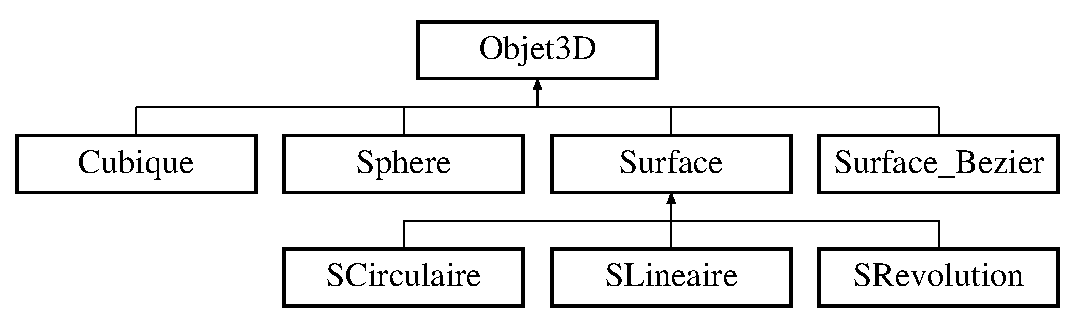
\includegraphics[height=3.000000cm]{classObjet3D}
\end{center}
\end{figure}
\subsection*{Public Member Functions}
\begin{DoxyCompactItemize}
\item 
\hyperlink{classObjet3D_aa378c3af15cbb46b010603f94c1d62f3}{Objet3\-D} (float largeur, float hauteur, float longueur)
\item 
virtual void \hyperlink{classObjet3D_adeb89dbb10335cd671378377818c1f71}{construction} ()
\item 
void \hyperlink{classObjet3D_ababe950dcc59f781b8140c327d64bdf6}{affiche\-Points} () const 
\item 
void \hyperlink{classObjet3D_a709f4a7ea16ecbf8628f41f0d701a211}{affichage} () const 
\item 
\hypertarget{classObjet3D_a1e0e07c88de765c1f303f65ab6c8d4c2}{{\bfseries Objet3\-D} (const \hyperlink{classObjet3D}{Objet3\-D} \&orig)}\label{classObjet3D_a1e0e07c88de765c1f303f65ab6c8d4c2}

\item 
float \hyperlink{classObjet3D_a0ea8e830e644ef96444969735679af66}{get\-Hauteur} () const 
\item 
float \hyperlink{classObjet3D_afaadd0060040977f410c5e0e724219c9}{get\-Largeur} () const 
\item 
float \hyperlink{classObjet3D_a8a364df4157ccde3eee4d544151a875b}{get\-Longeur} () const 
\item 
void \hyperlink{classObjet3D_ae8638f280f3627419c6777fe974011b2}{animation\-Lineaire} (std\-::vector$<$ \hyperlink{classPointGL}{Point\-G\-L} $\ast$ $>$ points\-Cles, float a)
\item 
std\-::vector$<$ \hyperlink{classPointGL}{Point\-G\-L} $\ast$ $>$ \hyperlink{classObjet3D_ad6212ed4caebf78e5a1764a2a3d76551}{get\-P} ()
\end{DoxyCompactItemize}
\subsection*{Protected Member Functions}
\begin{DoxyCompactItemize}
\item 
void \hyperlink{classObjet3D_a55b19161ab383c859dda77a43f7471fc}{calcule\-Normal} ()
\item 
void \hyperlink{classObjet3D_af4fb214001539392efb76b79a047c93e}{calcule\-Facette} ()
\end{DoxyCompactItemize}
\subsection*{Protected Attributes}
\begin{DoxyCompactItemize}
\item 
\hypertarget{classObjet3D_a69365378a5fae36f1e9f2fc7722fc4f5}{std\-::vector$<$ \hyperlink{classPointGL}{Point\-G\-L} $\ast$ $>$ {\bfseries points\-Referents}}\label{classObjet3D_a69365378a5fae36f1e9f2fc7722fc4f5}

\item 
\hypertarget{classObjet3D_a4ea8b7db42b1ba185f55ce49d3cdd13e}{std\-::vector$<$ \hyperlink{classPointGL}{Point\-G\-L} $\ast$ $>$ {\bfseries points}}\label{classObjet3D_a4ea8b7db42b1ba185f55ce49d3cdd13e}

\item 
\hypertarget{classObjet3D_a96937966af7a998d477ff60499f88e89}{std\-::vector$<$ \hyperlink{classTexel}{Texel} $\ast$ $>$ {\bfseries texels}}\label{classObjet3D_a96937966af7a998d477ff60499f88e89}

\item 
\hypertarget{classObjet3D_a910312e0c543bc5c1f423f713a841e9e}{std\-::vector$<$ \hyperlink{classFace}{Face} $\ast$ $>$ {\bfseries faces}}\label{classObjet3D_a910312e0c543bc5c1f423f713a841e9e}

\item 
\hypertarget{classObjet3D_afd0238a66814cdbf2fca0fc6afe89ff2}{float {\bfseries hauteur}}\label{classObjet3D_afd0238a66814cdbf2fca0fc6afe89ff2}

\item 
\hypertarget{classObjet3D_afcc95dcb6e9e0f85af4633bde1992da6}{float {\bfseries largeur}}\label{classObjet3D_afcc95dcb6e9e0f85af4633bde1992da6}

\item 
\hypertarget{classObjet3D_a02b4e577a1f81f5df155e5e94de71252}{float {\bfseries longueur}}\label{classObjet3D_a02b4e577a1f81f5df155e5e94de71252}

\item 
\hypertarget{classObjet3D_a7fb70f76d88b1dfbd32eb2d888bd321d}{\hyperlink{classMateriel}{Materiel} $\ast$ {\bfseries mat}}\label{classObjet3D_a7fb70f76d88b1dfbd32eb2d888bd321d}

\item 
\hypertarget{classObjet3D_a3a3b7dc321d2aed3e729595e6ec9cd85}{bool {\bfseries animation\-Active}}\label{classObjet3D_a3a3b7dc321d2aed3e729595e6ec9cd85}

\end{DoxyCompactItemize}


\subsection{Detailed Description}
\begin{DoxyAuthor}{Author}
P\-O\-N\-C\-I\-A\-N\-O Jean-\/\-Jacques et P\-R\-U\-D\-H\-O\-M\-M\-E Claire 
\end{DoxyAuthor}
\begin{DoxyDate}{Date}
13/03/2014
\end{DoxyDate}
Cette oeuvre, création, code, site ou texte est sous licence Creative Commons Attribution -\/ Pas d’\-Utilisation Commerciale -\/ Partage dans les Mêmes Conditions 4.\-0 International. Pour accéder à une copie de cette licence, merci de vous rendre à l'adresse suivante \href{http://creativecommons.org/licenses/by-nc-sa/4.0/deed.fr}{\tt http\-://creativecommons.\-org/licenses/by-\/nc-\/sa/4.\-0/deed.\-fr} ou envoyez un courrier à Creative Commons, 444 Castro Street, Suite 900, Mountain View, California, 94041, U\-S\-A. Copyright 2014

Contact\-: \href{mailto:ponciano.jeanjacques@gmail.com}{\tt ponciano.\-jeanjacques@gmail.\-com} 

\subsection{Constructor \& Destructor Documentation}
\hypertarget{classObjet3D_aa378c3af15cbb46b010603f94c1d62f3}{\index{Objet3\-D@{Objet3\-D}!Objet3\-D@{Objet3\-D}}
\index{Objet3\-D@{Objet3\-D}!Objet3D@{Objet3\-D}}
\subsubsection[{Objet3\-D}]{\setlength{\rightskip}{0pt plus 5cm}Objet3\-D\-::\-Objet3\-D (
\begin{DoxyParamCaption}
\item[{float}]{largeur, }
\item[{float}]{hauteur, }
\item[{float}]{longueur}
\end{DoxyParamCaption}
)}}\label{classObjet3D_aa378c3af15cbb46b010603f94c1d62f3}
Constructeur 
\begin{DoxyParams}{Parameters}
{\em largeur} & largeur de l'objet \\
\hline
{\em hauteur} & hauteur de l'objet \\
\hline
{\em longueur} & longueur de l'objet \\
\hline
\end{DoxyParams}


\subsection{Member Function Documentation}
\hypertarget{classObjet3D_a709f4a7ea16ecbf8628f41f0d701a211}{\index{Objet3\-D@{Objet3\-D}!affichage@{affichage}}
\index{affichage@{affichage}!Objet3D@{Objet3\-D}}
\subsubsection[{affichage}]{\setlength{\rightskip}{0pt plus 5cm}void Objet3\-D\-::affichage (
\begin{DoxyParamCaption}
{}
\end{DoxyParamCaption}
) const}}\label{classObjet3D_a709f4a7ea16ecbf8628f41f0d701a211}
Affiche l'objet sous forme de facette \hypertarget{classObjet3D_ababe950dcc59f781b8140c327d64bdf6}{\index{Objet3\-D@{Objet3\-D}!affiche\-Points@{affiche\-Points}}
\index{affiche\-Points@{affiche\-Points}!Objet3D@{Objet3\-D}}
\subsubsection[{affiche\-Points}]{\setlength{\rightskip}{0pt plus 5cm}void Objet3\-D\-::affiche\-Points (
\begin{DoxyParamCaption}
{}
\end{DoxyParamCaption}
) const}}\label{classObjet3D_ababe950dcc59f781b8140c327d64bdf6}
Affiche chaque point de l'objet \hypertarget{classObjet3D_ae8638f280f3627419c6777fe974011b2}{\index{Objet3\-D@{Objet3\-D}!animation\-Lineaire@{animation\-Lineaire}}
\index{animation\-Lineaire@{animation\-Lineaire}!Objet3D@{Objet3\-D}}
\subsubsection[{animation\-Lineaire}]{\setlength{\rightskip}{0pt plus 5cm}void Objet3\-D\-::animation\-Lineaire (
\begin{DoxyParamCaption}
\item[{std\-::vector$<$ {\bf Point\-G\-L} $\ast$ $>$}]{points\-Cles, }
\item[{float}]{a}
\end{DoxyParamCaption}
)}}\label{classObjet3D_ae8638f280f3627419c6777fe974011b2}
Animation de l'objets par interpolation linaire entre chaque points du tableau référent \char`\"{}points\-Referents\char`\"{} avec chaque point du tableau \char`\"{}points\-Cles\char`\"{} 
\begin{DoxyParams}{Parameters}
{\em points\-Cles} & tableau de points référent représentant une position clé de l'objet \\
\hline
{\em a} & vitesse d'avancement de l'interpolation linéaire. \\
\hline
\end{DoxyParams}
\hypertarget{classObjet3D_af4fb214001539392efb76b79a047c93e}{\index{Objet3\-D@{Objet3\-D}!calcule\-Facette@{calcule\-Facette}}
\index{calcule\-Facette@{calcule\-Facette}!Objet3D@{Objet3\-D}}
\subsubsection[{calcule\-Facette}]{\setlength{\rightskip}{0pt plus 5cm}void Objet3\-D\-::calcule\-Facette (
\begin{DoxyParamCaption}
{}
\end{DoxyParamCaption}
)\hspace{0.3cm}{\ttfamily [protected]}}}\label{classObjet3D_af4fb214001539392efb76b79a047c93e}
Calcule toutes les faces à partir du tableau de point \char`\"{}points\char`\"{} \hypertarget{classObjet3D_a55b19161ab383c859dda77a43f7471fc}{\index{Objet3\-D@{Objet3\-D}!calcule\-Normal@{calcule\-Normal}}
\index{calcule\-Normal@{calcule\-Normal}!Objet3D@{Objet3\-D}}
\subsubsection[{calcule\-Normal}]{\setlength{\rightskip}{0pt plus 5cm}void Objet3\-D\-::calcule\-Normal (
\begin{DoxyParamCaption}
{}
\end{DoxyParamCaption}
)\hspace{0.3cm}{\ttfamily [protected]}}}\label{classObjet3D_a55b19161ab383c859dda77a43f7471fc}
calcule les normales moyenne en chaque sommet. A exécuter impérativement à la fin de la construction de l'objet \hypertarget{classObjet3D_adeb89dbb10335cd671378377818c1f71}{\index{Objet3\-D@{Objet3\-D}!construction@{construction}}
\index{construction@{construction}!Objet3D@{Objet3\-D}}
\subsubsection[{construction}]{\setlength{\rightskip}{0pt plus 5cm}void Objet3\-D\-::construction (
\begin{DoxyParamCaption}
{}
\end{DoxyParamCaption}
)\hspace{0.3cm}{\ttfamily [virtual]}}}\label{classObjet3D_adeb89dbb10335cd671378377818c1f71}
Calcule tous les points de l'objet 

Reimplemented in \hyperlink{classSphere_a60631bd7158f7c443ebc5bda6066d2a2}{Sphere}, \hyperlink{classSLineaire_a3c82b3b19ad80e6815ca86cbb23facb9}{S\-Lineaire}, \hyperlink{classSCirculaire_a7db7e11fa18f5e00b870d7c062427572}{S\-Circulaire}, and \hyperlink{classSurface_a1beede80574f15acea63245d8c1149a3}{Surface}.

\hypertarget{classObjet3D_a0ea8e830e644ef96444969735679af66}{\index{Objet3\-D@{Objet3\-D}!get\-Hauteur@{get\-Hauteur}}
\index{get\-Hauteur@{get\-Hauteur}!Objet3D@{Objet3\-D}}
\subsubsection[{get\-Hauteur}]{\setlength{\rightskip}{0pt plus 5cm}float Objet3\-D\-::get\-Hauteur (
\begin{DoxyParamCaption}
{}
\end{DoxyParamCaption}
) const}}\label{classObjet3D_a0ea8e830e644ef96444969735679af66}
Récupération de la hauteur de l'objet \begin{DoxyReturn}{Returns}
hauteur de l'objet 
\end{DoxyReturn}
\hypertarget{classObjet3D_afaadd0060040977f410c5e0e724219c9}{\index{Objet3\-D@{Objet3\-D}!get\-Largeur@{get\-Largeur}}
\index{get\-Largeur@{get\-Largeur}!Objet3D@{Objet3\-D}}
\subsubsection[{get\-Largeur}]{\setlength{\rightskip}{0pt plus 5cm}float Objet3\-D\-::get\-Largeur (
\begin{DoxyParamCaption}
{}
\end{DoxyParamCaption}
) const}}\label{classObjet3D_afaadd0060040977f410c5e0e724219c9}
Récupération de la largeur de l'objet \begin{DoxyReturn}{Returns}
largeur de l'objet 
\end{DoxyReturn}
\hypertarget{classObjet3D_a8a364df4157ccde3eee4d544151a875b}{\index{Objet3\-D@{Objet3\-D}!get\-Longeur@{get\-Longeur}}
\index{get\-Longeur@{get\-Longeur}!Objet3D@{Objet3\-D}}
\subsubsection[{get\-Longeur}]{\setlength{\rightskip}{0pt plus 5cm}float Objet3\-D\-::get\-Longeur (
\begin{DoxyParamCaption}
{}
\end{DoxyParamCaption}
) const}}\label{classObjet3D_a8a364df4157ccde3eee4d544151a875b}
Récupération de la longueur de l'objet \begin{DoxyReturn}{Returns}
longueur de l'objet 
\end{DoxyReturn}
\hypertarget{classObjet3D_ad6212ed4caebf78e5a1764a2a3d76551}{\index{Objet3\-D@{Objet3\-D}!get\-P@{get\-P}}
\index{get\-P@{get\-P}!Objet3D@{Objet3\-D}}
\subsubsection[{get\-P}]{\setlength{\rightskip}{0pt plus 5cm}std\-::vector$<$ {\bf Point\-G\-L} $\ast$ $>$ Objet3\-D\-::get\-P (
\begin{DoxyParamCaption}
{}
\end{DoxyParamCaption}
)}}\label{classObjet3D_ad6212ed4caebf78e5a1764a2a3d76551}
Accesseur en lecture au tableau de points \begin{DoxyReturn}{Returns}
le tableau contenant les points de l'objet3\-D 
\end{DoxyReturn}


The documentation for this class was generated from the following files\-:\begin{DoxyCompactItemize}
\item 
modules/open\-G\-L/tools\-\_\-models/Objet3\-D.\-h\item 
modules/open\-G\-L/tools\-\_\-models/Objet3\-D.\-cpp\end{DoxyCompactItemize}

\hypertarget{classObjets}{\section{Objets Class Reference}
\label{classObjets}\index{Objets@{Objets}}
}


{\ttfamily \#include $<$Objets.\-h$>$}

Inheritance diagram for Objets\-:\begin{figure}[H]
\begin{center}
\leavevmode
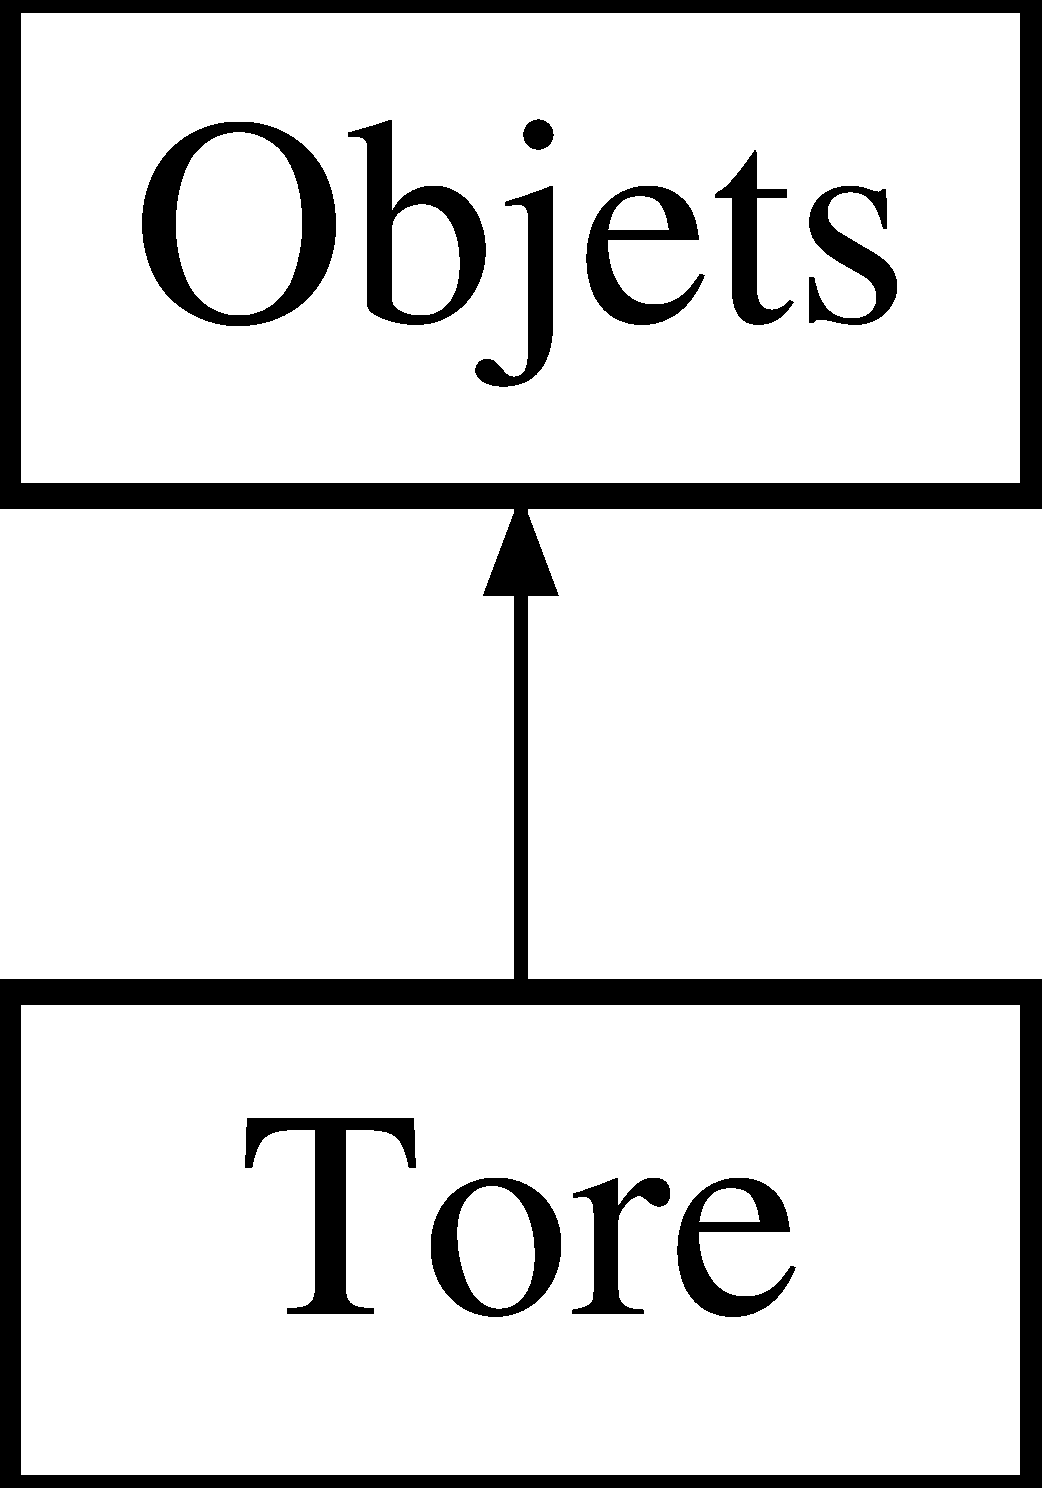
\includegraphics[height=2.000000cm]{classObjets}
\end{center}
\end{figure}
\subsection*{Public Member Functions}
\begin{DoxyCompactItemize}
\item 
virtual void \hyperlink{classObjets_a2c14a4a3841d82cef1d1ef4e695859f6}{construction} ()
\item 
void \hyperlink{classObjets_a33ab9a220bba2d8266901b1302d5d0e6}{affiche\-Points} () const 
\item 
void \hyperlink{classObjets_a0897b019b260a1b858dffd4fa07595fb}{affichage} () const 
\item 
void \hyperlink{classObjets_af830ffcb0d208607b530c80a9403f084}{set\-Texture} (\hyperlink{classTexture}{Texture} $\ast$text)
\item 
\hypertarget{classObjets_a63d846ef70e1d0922f79e16d77f0c7cb}{{\bfseries Objets} (const \hyperlink{classObjets}{Objets} \&orig)}\label{classObjets_a63d846ef70e1d0922f79e16d77f0c7cb}

\end{DoxyCompactItemize}
\subsection*{Protected Member Functions}
\begin{DoxyCompactItemize}
\item 
void \hyperlink{classObjets_ae481b18cf3a384d177d62a101b8df518}{calcule\-Normal} ()
\end{DoxyCompactItemize}
\subsection*{Protected Attributes}
\begin{DoxyCompactItemize}
\item 
\hypertarget{classObjets_a626af9cb2c818f96ee1107162bc88db1}{std\-::vector$<$ \hyperlink{classPointGL}{Point\-G\-L} $\ast$ $>$ {\bfseries points}}\label{classObjets_a626af9cb2c818f96ee1107162bc88db1}

\item 
\hypertarget{classObjets_aa12179399b8fa417a47cf9399e5746b7}{std\-::vector$<$ \hyperlink{classTexel}{Texel} $\ast$ $>$ {\bfseries texels}}\label{classObjets_aa12179399b8fa417a47cf9399e5746b7}

\item 
\hypertarget{classObjets_aba91b138535fd2825b1616af8c22fe68}{std\-::vector$<$ \hyperlink{classFace}{Face} $\ast$ $>$ {\bfseries faces}}\label{classObjets_aba91b138535fd2825b1616af8c22fe68}

\item 
\hypertarget{classObjets_aaf5fb81127ec1fdfbea5187079bdc408}{\hyperlink{classTexture}{Texture} $\ast$ {\bfseries t}}\label{classObjets_aaf5fb81127ec1fdfbea5187079bdc408}

\item 
\hypertarget{classObjets_a6047da5af8aa69b393b76e10f16aaebf}{bool {\bfseries texture\-Active}}\label{classObjets_a6047da5af8aa69b393b76e10f16aaebf}

\end{DoxyCompactItemize}


\subsection{Detailed Description}
\begin{DoxyAuthor}{Author}
P\-O\-N\-C\-I\-A\-N\-O Jean-\/\-Jacques et P\-R\-U\-D\-H\-O\-M\-M\-E Claire 
\end{DoxyAuthor}
\begin{DoxyDate}{Date}
13/03/2014
\end{DoxyDate}
Cette oeuvre, création, code, site ou texte est sous licence Creative Commons Attribution -\/ Pas d’\-Utilisation Commerciale -\/ Partage dans les Mêmes Conditions 4.\-0 International. Pour accéder à une copie de cette licence, merci de vous rendre à l'adresse suivante \href{http://creativecommons.org/licenses/by-nc-sa/4.0/deed.fr}{\tt http\-://creativecommons.\-org/licenses/by-\/nc-\/sa/4.\-0/deed.\-fr} ou envoyez un courrier à Creative Commons, 444 Castro Street, Suite 900, Mountain View, California, 94041, U\-S\-A. Copyright 2014

Contact\-: \href{mailto:ponciano.jeanjacques@gmail.com}{\tt ponciano.\-jeanjacques@gmail.\-com} 

\subsection{Member Function Documentation}
\hypertarget{classObjets_a0897b019b260a1b858dffd4fa07595fb}{\index{Objets@{Objets}!affichage@{affichage}}
\index{affichage@{affichage}!Objets@{Objets}}
\subsubsection[{affichage}]{\setlength{\rightskip}{0pt plus 5cm}void Objets\-::affichage (
\begin{DoxyParamCaption}
{}
\end{DoxyParamCaption}
) const}}\label{classObjets_a0897b019b260a1b858dffd4fa07595fb}
Affiche l'objet sous forme de facette \hypertarget{classObjets_a33ab9a220bba2d8266901b1302d5d0e6}{\index{Objets@{Objets}!affiche\-Points@{affiche\-Points}}
\index{affiche\-Points@{affiche\-Points}!Objets@{Objets}}
\subsubsection[{affiche\-Points}]{\setlength{\rightskip}{0pt plus 5cm}void Objets\-::affiche\-Points (
\begin{DoxyParamCaption}
{}
\end{DoxyParamCaption}
) const}}\label{classObjets_a33ab9a220bba2d8266901b1302d5d0e6}
Affiche chaque point de l'objet \hypertarget{classObjets_ae481b18cf3a384d177d62a101b8df518}{\index{Objets@{Objets}!calcule\-Normal@{calcule\-Normal}}
\index{calcule\-Normal@{calcule\-Normal}!Objets@{Objets}}
\subsubsection[{calcule\-Normal}]{\setlength{\rightskip}{0pt plus 5cm}void Objets\-::calcule\-Normal (
\begin{DoxyParamCaption}
{}
\end{DoxyParamCaption}
)\hspace{0.3cm}{\ttfamily [protected]}}}\label{classObjets_ae481b18cf3a384d177d62a101b8df518}
calcule les normales moyenne en chaque sommet. A exécuter impérativement à la fin de la construction de l'objet \hypertarget{classObjets_a2c14a4a3841d82cef1d1ef4e695859f6}{\index{Objets@{Objets}!construction@{construction}}
\index{construction@{construction}!Objets@{Objets}}
\subsubsection[{construction}]{\setlength{\rightskip}{0pt plus 5cm}void Objets\-::construction (
\begin{DoxyParamCaption}
{}
\end{DoxyParamCaption}
)\hspace{0.3cm}{\ttfamily [virtual]}}}\label{classObjets_a2c14a4a3841d82cef1d1ef4e695859f6}
Calcule tous les points de l'objet 

Reimplemented in \hyperlink{classTore_acfda6ef660e1a3f3f8c9e78cdb63a629}{Tore}.

\hypertarget{classObjets_af830ffcb0d208607b530c80a9403f084}{\index{Objets@{Objets}!set\-Texture@{set\-Texture}}
\index{set\-Texture@{set\-Texture}!Objets@{Objets}}
\subsubsection[{set\-Texture}]{\setlength{\rightskip}{0pt plus 5cm}void Objets\-::set\-Texture (
\begin{DoxyParamCaption}
\item[{{\bf Texture} $\ast$}]{text}
\end{DoxyParamCaption}
)}}\label{classObjets_af830ffcb0d208607b530c80a9403f084}
Changement de texture 
\begin{DoxyParams}{Parameters}
{\em text} & nouvelle texture à affecter \\
\hline
\end{DoxyParams}


The documentation for this class was generated from the following files\-:\begin{DoxyCompactItemize}
\item 
modules/open\-G\-L/tools\-\_\-models/Objets.\-h\item 
modules/open\-G\-L/tools\-\_\-models/Objets.\-cpp\end{DoxyCompactItemize}

\hypertarget{classPointGL}{\section{Point\-G\-L Class Reference}
\label{classPointGL}\index{Point\-G\-L@{Point\-G\-L}}
}


{\ttfamily \#include $<$Point.\-h$>$}

\subsection*{Public Member Functions}
\begin{DoxyCompactItemize}
\item 
\hyperlink{classPointGL_a24e4ffa65772815aa20753e0bc786172}{Point\-G\-L} ()
\item 
\hyperlink{classPointGL_a7c78587e20818ba1cf6101d84c209f30}{Point\-G\-L} (float x, float y, float z)
\item 
\hypertarget{classPointGL_ad43d1643664e6e534a5e254628c1c9c9}{{\bfseries Point\-G\-L} (const \hyperlink{classPointGL}{Point\-G\-L} \&orig)}\label{classPointGL_ad43d1643664e6e534a5e254628c1c9c9}

\item 
float \hyperlink{classPointGL_adb7aa72a985bdd393e896a1414826cc4}{get\-X} () const 
\item 
float \hyperlink{classPointGL_a6808f21ba18339ebcb7ed085748a0ab2}{get\-Y} () const 
\item 
float \hyperlink{classPointGL_a6ca34827d4db24440f77695916952035}{get\-Z} () const 
\item 
void \hyperlink{classPointGL_af3a2a263da2b88f6878b9129ed3c89dd}{set\-X} (float a)
\item 
void \hyperlink{classPointGL_a9db09a7eea4bd0b1c674477d17c57ca8}{set\-Y} (float a)
\item 
void \hyperlink{classPointGL_ae9fee8c6d9bf2c9de0edaaee1cb1c210}{set\-Z} (float a)
\item 
void \hyperlink{classPointGL_a6997b9b1af305d3826e02a3809b1dead}{set\-Normal\-Moyenne} (std\-::vector$<$ float $>$n)
\item 
void \hyperlink{classPointGL_a62e96c2dfcd8a8b8c393b6306dff76cc}{set\-Normal\-Moyenne} (float x, float y, float z)
\item 
std\-::vector$<$ float $>$ \hyperlink{classPointGL_a93f7846dd282e0352349c2905ccbf6f3}{get\-Normal} () const 
\item 
void \hyperlink{classPointGL_aba253aa08f7f222d5d7355191875bc35}{translation} (float x, float y, float z)
\item 
void \hyperlink{classPointGL_ae50ee0f316b8b1e292f47c3c4e8460fa}{rotation} (float a, int x, int y, int z)
\item 
void \hyperlink{classPointGL_a2a664d07bcb24bebaeca3e9ac3d5586f}{scale} (float x, float y, float z)
\end{DoxyCompactItemize}


\subsection{Detailed Description}
\begin{DoxyAuthor}{Author}
P\-O\-N\-C\-I\-A\-N\-O Jean-\/\-Jacques et P\-R\-U\-D\-H\-O\-M\-M\-E Claire 
\end{DoxyAuthor}
\begin{DoxyDate}{Date}
13/03/2014
\end{DoxyDate}
Cette oeuvre, création, code, site ou texte est sous licence Creative Commons Attribution -\/ Pas d’\-Utilisation Commerciale -\/ Partage dans les Mêmes Conditions 4.\-0 International. Pour accéder à une copie de cette licence, merci de vous rendre à l'adresse suivante \href{http://creativecommons.org/licenses/by-nc-sa/4.0/deed.fr}{\tt http\-://creativecommons.\-org/licenses/by-\/nc-\/sa/4.\-0/deed.\-fr} ou envoyez un courrier à Creative Commons, 444 Castro Street, Suite 900, Mountain View, California, 94041, U\-S\-A. Copyright 2014

Contact\-: \href{mailto:ponciano.jeanjacques@gmail.com}{\tt ponciano.\-jeanjacques@gmail.\-com} 

\subsection{Constructor \& Destructor Documentation}
\hypertarget{classPointGL_a24e4ffa65772815aa20753e0bc786172}{\index{Point\-G\-L@{Point\-G\-L}!Point\-G\-L@{Point\-G\-L}}
\index{Point\-G\-L@{Point\-G\-L}!PointGL@{Point\-G\-L}}
\subsubsection[{Point\-G\-L}]{\setlength{\rightskip}{0pt plus 5cm}Point\-G\-L\-::\-Point\-G\-L (
\begin{DoxyParamCaption}
{}
\end{DoxyParamCaption}
)}}\label{classPointGL_a24e4ffa65772815aa20753e0bc786172}
Construteur par défaut construisant le point à l'origine du repère \hypertarget{classPointGL_a7c78587e20818ba1cf6101d84c209f30}{\index{Point\-G\-L@{Point\-G\-L}!Point\-G\-L@{Point\-G\-L}}
\index{Point\-G\-L@{Point\-G\-L}!PointGL@{Point\-G\-L}}
\subsubsection[{Point\-G\-L}]{\setlength{\rightskip}{0pt plus 5cm}Point\-G\-L\-::\-Point\-G\-L (
\begin{DoxyParamCaption}
\item[{float}]{x, }
\item[{float}]{y, }
\item[{float}]{z}
\end{DoxyParamCaption}
)}}\label{classPointGL_a7c78587e20818ba1cf6101d84c209f30}
Construction du point 
\begin{DoxyParams}{Parameters}
{\em x} & abscisse \\
\hline
{\em y} & ordonnée \\
\hline
{\em z} & profondeur \\
\hline
\end{DoxyParams}


\subsection{Member Function Documentation}
\hypertarget{classPointGL_a93f7846dd282e0352349c2905ccbf6f3}{\index{Point\-G\-L@{Point\-G\-L}!get\-Normal@{get\-Normal}}
\index{get\-Normal@{get\-Normal}!PointGL@{Point\-G\-L}}
\subsubsection[{get\-Normal}]{\setlength{\rightskip}{0pt plus 5cm}std\-::vector$<$ float $>$ Point\-G\-L\-::get\-Normal (
\begin{DoxyParamCaption}
{}
\end{DoxyParamCaption}
) const}}\label{classPointGL_a93f7846dd282e0352349c2905ccbf6f3}
Récupération du vecteur normal à la face \begin{DoxyReturn}{Returns}
le vecteur normal 
\end{DoxyReturn}
\hypertarget{classPointGL_adb7aa72a985bdd393e896a1414826cc4}{\index{Point\-G\-L@{Point\-G\-L}!get\-X@{get\-X}}
\index{get\-X@{get\-X}!PointGL@{Point\-G\-L}}
\subsubsection[{get\-X}]{\setlength{\rightskip}{0pt plus 5cm}float Point\-G\-L\-::get\-X (
\begin{DoxyParamCaption}
{}
\end{DoxyParamCaption}
) const}}\label{classPointGL_adb7aa72a985bdd393e896a1414826cc4}
Récupération de l'abscisse du point \begin{DoxyReturn}{Returns}
abscisse du point 
\end{DoxyReturn}
\hypertarget{classPointGL_a6808f21ba18339ebcb7ed085748a0ab2}{\index{Point\-G\-L@{Point\-G\-L}!get\-Y@{get\-Y}}
\index{get\-Y@{get\-Y}!PointGL@{Point\-G\-L}}
\subsubsection[{get\-Y}]{\setlength{\rightskip}{0pt plus 5cm}float Point\-G\-L\-::get\-Y (
\begin{DoxyParamCaption}
{}
\end{DoxyParamCaption}
) const}}\label{classPointGL_a6808f21ba18339ebcb7ed085748a0ab2}
Récupération de l'ordonnée du point \begin{DoxyReturn}{Returns}
ordonnée du point 
\end{DoxyReturn}
\hypertarget{classPointGL_a6ca34827d4db24440f77695916952035}{\index{Point\-G\-L@{Point\-G\-L}!get\-Z@{get\-Z}}
\index{get\-Z@{get\-Z}!PointGL@{Point\-G\-L}}
\subsubsection[{get\-Z}]{\setlength{\rightskip}{0pt plus 5cm}float Point\-G\-L\-::get\-Z (
\begin{DoxyParamCaption}
{}
\end{DoxyParamCaption}
) const}}\label{classPointGL_a6ca34827d4db24440f77695916952035}
Récupération de la profondeur du point \begin{DoxyReturn}{Returns}
profondeur du point 
\end{DoxyReturn}
\hypertarget{classPointGL_ae50ee0f316b8b1e292f47c3c4e8460fa}{\index{Point\-G\-L@{Point\-G\-L}!rotation@{rotation}}
\index{rotation@{rotation}!PointGL@{Point\-G\-L}}
\subsubsection[{rotation}]{\setlength{\rightskip}{0pt plus 5cm}void Point\-G\-L\-::rotation (
\begin{DoxyParamCaption}
\item[{float}]{a, }
\item[{int}]{x, }
\item[{int}]{y, }
\item[{int}]{z}
\end{DoxyParamCaption}
)}}\label{classPointGL_ae50ee0f316b8b1e292f47c3c4e8460fa}
Opération de rotation 
\begin{DoxyParams}{Parameters}
{\em angle} & angle de rotation \\
\hline
{\em x} & axe de rotation \\
\hline
{\em y} & axe de rotation \\
\hline
{\em z} & axe de rotation \\
\hline
\end{DoxyParams}
\hypertarget{classPointGL_a2a664d07bcb24bebaeca3e9ac3d5586f}{\index{Point\-G\-L@{Point\-G\-L}!scale@{scale}}
\index{scale@{scale}!PointGL@{Point\-G\-L}}
\subsubsection[{scale}]{\setlength{\rightskip}{0pt plus 5cm}void Point\-G\-L\-::scale (
\begin{DoxyParamCaption}
\item[{float}]{x, }
\item[{float}]{y, }
\item[{float}]{z}
\end{DoxyParamCaption}
)}}\label{classPointGL_a2a664d07bcb24bebaeca3e9ac3d5586f}
Opération de mise à l'échelle 
\begin{DoxyParams}{Parameters}
{\em x} & \\
\hline
{\em y} & \\
\hline
{\em z} & \\
\hline
\end{DoxyParams}
\hypertarget{classPointGL_a6997b9b1af305d3826e02a3809b1dead}{\index{Point\-G\-L@{Point\-G\-L}!set\-Normal\-Moyenne@{set\-Normal\-Moyenne}}
\index{set\-Normal\-Moyenne@{set\-Normal\-Moyenne}!PointGL@{Point\-G\-L}}
\subsubsection[{set\-Normal\-Moyenne}]{\setlength{\rightskip}{0pt plus 5cm}void Point\-G\-L\-::set\-Normal\-Moyenne (
\begin{DoxyParamCaption}
\item[{std\-::vector$<$ float $>$}]{n}
\end{DoxyParamCaption}
)}}\label{classPointGL_a6997b9b1af305d3826e02a3809b1dead}
Modifie la valeur de la normal moyenne en ce point 
\begin{DoxyParams}{Parameters}
{\em n} & normale moyenne à affecter \\
\hline
\end{DoxyParams}
\hypertarget{classPointGL_a62e96c2dfcd8a8b8c393b6306dff76cc}{\index{Point\-G\-L@{Point\-G\-L}!set\-Normal\-Moyenne@{set\-Normal\-Moyenne}}
\index{set\-Normal\-Moyenne@{set\-Normal\-Moyenne}!PointGL@{Point\-G\-L}}
\subsubsection[{set\-Normal\-Moyenne}]{\setlength{\rightskip}{0pt plus 5cm}void Point\-G\-L\-::set\-Normal\-Moyenne (
\begin{DoxyParamCaption}
\item[{float}]{x, }
\item[{float}]{y, }
\item[{float}]{z}
\end{DoxyParamCaption}
)}}\label{classPointGL_a62e96c2dfcd8a8b8c393b6306dff76cc}
Modifie la valeur de la normal moyenne en ce point 
\begin{DoxyParams}{Parameters}
{\em x} & \\
\hline
{\em y} & \\
\hline
{\em z} & \\
\hline
\end{DoxyParams}
\hypertarget{classPointGL_af3a2a263da2b88f6878b9129ed3c89dd}{\index{Point\-G\-L@{Point\-G\-L}!set\-X@{set\-X}}
\index{set\-X@{set\-X}!PointGL@{Point\-G\-L}}
\subsubsection[{set\-X}]{\setlength{\rightskip}{0pt plus 5cm}void Point\-G\-L\-::set\-X (
\begin{DoxyParamCaption}
\item[{float}]{a}
\end{DoxyParamCaption}
)}}\label{classPointGL_af3a2a263da2b88f6878b9129ed3c89dd}
Modification de l'abscisse du point 
\begin{DoxyParams}{Parameters}
{\em a} & nouvel abscisse \\
\hline
\end{DoxyParams}
\hypertarget{classPointGL_a9db09a7eea4bd0b1c674477d17c57ca8}{\index{Point\-G\-L@{Point\-G\-L}!set\-Y@{set\-Y}}
\index{set\-Y@{set\-Y}!PointGL@{Point\-G\-L}}
\subsubsection[{set\-Y}]{\setlength{\rightskip}{0pt plus 5cm}void Point\-G\-L\-::set\-Y (
\begin{DoxyParamCaption}
\item[{float}]{a}
\end{DoxyParamCaption}
)}}\label{classPointGL_a9db09a7eea4bd0b1c674477d17c57ca8}
Modification de l'ordonné du point 
\begin{DoxyParams}{Parameters}
{\em a} & nouvel ordonné \\
\hline
\end{DoxyParams}
\hypertarget{classPointGL_ae9fee8c6d9bf2c9de0edaaee1cb1c210}{\index{Point\-G\-L@{Point\-G\-L}!set\-Z@{set\-Z}}
\index{set\-Z@{set\-Z}!PointGL@{Point\-G\-L}}
\subsubsection[{set\-Z}]{\setlength{\rightskip}{0pt plus 5cm}void Point\-G\-L\-::set\-Z (
\begin{DoxyParamCaption}
\item[{float}]{a}
\end{DoxyParamCaption}
)}}\label{classPointGL_ae9fee8c6d9bf2c9de0edaaee1cb1c210}
Modification de la prodondeur du point 
\begin{DoxyParams}{Parameters}
{\em a} & nouvelle prodondeur \\
\hline
\end{DoxyParams}
\hypertarget{classPointGL_aba253aa08f7f222d5d7355191875bc35}{\index{Point\-G\-L@{Point\-G\-L}!translation@{translation}}
\index{translation@{translation}!PointGL@{Point\-G\-L}}
\subsubsection[{translation}]{\setlength{\rightskip}{0pt plus 5cm}void Point\-G\-L\-::translation (
\begin{DoxyParamCaption}
\item[{float}]{x, }
\item[{float}]{y, }
\item[{float}]{z}
\end{DoxyParamCaption}
)}}\label{classPointGL_aba253aa08f7f222d5d7355191875bc35}
Opération de translation 
\begin{DoxyParams}{Parameters}
{\em x} & \\
\hline
{\em y} & \\
\hline
{\em z} & \\
\hline
\end{DoxyParams}


The documentation for this class was generated from the following files\-:\begin{DoxyCompactItemize}
\item 
modules/open\-G\-L/tools\-\_\-models/Point.\-h\item 
modules/open\-G\-L/tools\-\_\-models/Point.\-cpp\end{DoxyCompactItemize}

\hypertarget{classScene}{\section{Scene Class Reference}
\label{classScene}\index{Scene@{Scene}}
}


{\ttfamily \#include $<$Scene.\-h$>$}

\subsection*{Public Member Functions}
\begin{DoxyCompactItemize}
\item 
\hyperlink{classScene_ad10176d75a9cc0da56626f682d083507}{Scene} ()
\item 
\hypertarget{classScene_a44eef26bfd4ff2196c0689d30d651ac0}{{\bfseries Scene} (const \hyperlink{classScene}{Scene} \&orig)}\label{classScene_a44eef26bfd4ff2196c0689d30d651ac0}

\item 
void \hyperlink{classScene_a278d69cec31d0f217f66d6d5b835c1cf}{initialisation} ()
\item 
void \hyperlink{classScene_a21d0fc2e44e61436e2434790c71e6d79}{clavier} (int touche)
\item 
void \hyperlink{classScene_af43ee036671541ec134792751a57a83f}{mouse\-Clicked} (Q\-Mouse\-Event $\ast$event)
\begin{DoxyCompactList}\small\item\em mouse \end{DoxyCompactList}\item 
void \hyperlink{classScene_af8819619897d14c6e58655252d4c5f37}{mousemotion} (int x, int y)
\item 
void \hyperlink{classScene_aeb3584af02d5818a17ea91eb5d19fc92}{affichage} ()
\item 
void \hyperlink{classScene_a76bd2b46fa79e3a939ea87c9da2d8928}{eclairage} (bool e)
\item 
void \hyperlink{classScene_a38a063de5f88ffefc9a7ef90e9ba23cb}{lumiere} ()
\item 
void \hyperlink{classScene_aaea9ff8b946f2d004037b116e5a53f08}{spot} (G\-Lenum lum)
\item 
void \hyperlink{classScene_a576e0cdbd359e0888ba33d2f004365c3}{grille} () const 
\item 
void \hyperlink{classScene_a5e9920a83e80a09a255c8c17052b1313}{animation\-Lineaire} (float px, float py, float pz, float lx, float ly, float lz, float zoome, float a)
\item 
void \hyperlink{classScene_ab546e6e73c981e816c95c96436f86a4f}{deplacement} (int touche)
\item 
void \hyperlink{classScene_af64db0a4c0a5986b12624caefaf6d6e4}{set\-Camera\-Location} (int x, int y, int z)
\begin{DoxyCompactList}\small\item\em set\-Camera\-Location permet d'affecter de nouvelles coordonnées à la caméra \end{DoxyCompactList}\item 
void \hyperlink{classScene_ac9e914eb62fd1520fd3ad0000f2015de}{set\-Camera\-Look\-At} (int x, int y, int z)
\begin{DoxyCompactList}\small\item\em set\-Camera\-Look\-At permet d'affecter de nouvelles coordonnées au point de visé de la caméra \end{DoxyCompactList}\item 
float \hyperlink{classScene_a77b47fda37a4f654c2afc1369243cc71}{get\-Posx} ()
\begin{DoxyCompactList}\small\item\em get\-Posx \end{DoxyCompactList}\item 
float \hyperlink{classScene_ae519821e00f9f4022fe01e27f29341b1}{get\-Posy} ()
\begin{DoxyCompactList}\small\item\em get\-Posy \end{DoxyCompactList}\item 
float \hyperlink{classScene_a5bc3326488d3899234b900362cc3922e}{get\-Posz} ()
\begin{DoxyCompactList}\small\item\em get\-Posz \end{DoxyCompactList}\item 
float \hyperlink{classScene_ab1c2fef33054817bbede5a4048e4c40e}{get\-Lookx} ()
\begin{DoxyCompactList}\small\item\em get\-Lookx \end{DoxyCompactList}\item 
float \hyperlink{classScene_a8ec463670f863914c2398fe21143d0e6}{get\-Looky} ()
\begin{DoxyCompactList}\small\item\em get\-Looky \end{DoxyCompactList}\item 
float \hyperlink{classScene_a3b5b9bdd1371ed2330ab9e2bf39456a7}{get\-Lookz} ()
\begin{DoxyCompactList}\small\item\em get\-Lookz \end{DoxyCompactList}\item 
\hypertarget{classScene_ade754942bbdec763bbf3f8d0595fde04}{void {\bfseries zoom} ()}\label{classScene_ade754942bbdec763bbf3f8d0595fde04}

\item 
\hypertarget{classScene_a79ba6db33b5fbac304c9f6811da42b0b}{void {\bfseries dezoom} ()}\label{classScene_a79ba6db33b5fbac304c9f6811da42b0b}

\item 
\hypertarget{classScene_ae6393370d5cc51ecc620c60597dc3853}{void {\bfseries reset} ()}\label{classScene_ae6393370d5cc51ecc620c60597dc3853}

\end{DoxyCompactItemize}


\subsection{Detailed Description}
\begin{DoxyAuthor}{Author}
P\-O\-N\-C\-I\-A\-N\-O Jean-\/\-Jacques et P\-R\-U\-D\-H\-O\-M\-M\-E Claire 
\end{DoxyAuthor}
\begin{DoxyDate}{Date}
13/03/2014
\end{DoxyDate}
Cette oeuvre, création, code, site ou texte est sous licence Creative Commons Attribution -\/ Pas d’\-Utilisation Commerciale -\/ Partage dans les Mêmes Conditions 4.\-0 International. Pour accéder à une copie de cette licence, merci de vous rendre à l'adresse suivante \href{http://creativecommons.org/licenses/by-nc-sa/4.0/deed.fr}{\tt http\-://creativecommons.\-org/licenses/by-\/nc-\/sa/4.\-0/deed.\-fr} ou envoyez un courrier à Creative Commons, 444 Castro Street, Suite 900, Mountain View, California, 94041, U\-S\-A. Copyright 2014

Contact\-: \href{mailto:ponciano.jeanjacques@gmail.com}{\tt ponciano.\-jeanjacques@gmail.\-com} 

\subsection{Constructor \& Destructor Documentation}
\hypertarget{classScene_ad10176d75a9cc0da56626f682d083507}{\index{Scene@{Scene}!Scene@{Scene}}
\index{Scene@{Scene}!Scene@{Scene}}
\subsubsection[{Scene}]{\setlength{\rightskip}{0pt plus 5cm}Scene\-::\-Scene (
\begin{DoxyParamCaption}
{}
\end{DoxyParamCaption}
)}}\label{classScene_ad10176d75a9cc0da56626f682d083507}
Constructeur 

\subsection{Member Function Documentation}
\hypertarget{classScene_aeb3584af02d5818a17ea91eb5d19fc92}{\index{Scene@{Scene}!affichage@{affichage}}
\index{affichage@{affichage}!Scene@{Scene}}
\subsubsection[{affichage}]{\setlength{\rightskip}{0pt plus 5cm}void Scene\-::affichage (
\begin{DoxyParamCaption}
{}
\end{DoxyParamCaption}
)}}\label{classScene_aeb3584af02d5818a17ea91eb5d19fc92}
Affichage minimaliste de la scène \hypertarget{classScene_a5e9920a83e80a09a255c8c17052b1313}{\index{Scene@{Scene}!animation\-Lineaire@{animation\-Lineaire}}
\index{animation\-Lineaire@{animation\-Lineaire}!Scene@{Scene}}
\subsubsection[{animation\-Lineaire}]{\setlength{\rightskip}{0pt plus 5cm}void Scene\-::animation\-Lineaire (
\begin{DoxyParamCaption}
\item[{float}]{px, }
\item[{float}]{py, }
\item[{float}]{pz, }
\item[{float}]{lx, }
\item[{float}]{ly, }
\item[{float}]{lz, }
\item[{float}]{zoome, }
\item[{float}]{a}
\end{DoxyParamCaption}
)}}\label{classScene_a5e9920a83e80a09a255c8c17052b1313}
Interpolation par image cré avec la caméra 
\begin{DoxyParams}{Parameters}
{\em px} & abscisse de la position de l'image clé de la caméra \\
\hline
{\em py} & ordonnée de la position de l'image clé de la caméra \\
\hline
{\em pz} & profondeur de la position de l'image clé de la caméra \\
\hline
{\em lx} & abscisse de la position de l'image clé de la caméra \\
\hline
{\em ly} & ordonnée de la position de l'image clé de la caméra \\
\hline
{\em lz} & profondeur de la position de l'image clé de la caméra \\
\hline
{\em zoome} & zoome de la caméra \\
\hline
{\em a} & avancement de l'interpolation linéaire \\
\hline
\end{DoxyParams}
\hypertarget{classScene_a21d0fc2e44e61436e2434790c71e6d79}{\index{Scene@{Scene}!clavier@{clavier}}
\index{clavier@{clavier}!Scene@{Scene}}
\subsubsection[{clavier}]{\setlength{\rightskip}{0pt plus 5cm}void Scene\-::clavier (
\begin{DoxyParamCaption}
\item[{int}]{touche}
\end{DoxyParamCaption}
)}}\label{classScene_a21d0fc2e44e61436e2434790c71e6d79}
Traitement des actions effectué avec le clavier 
\begin{DoxyParams}{Parameters}
{\em touche} & touche pressée \\
\hline
\end{DoxyParams}
\hypertarget{classScene_ab546e6e73c981e816c95c96436f86a4f}{\index{Scene@{Scene}!deplacement@{deplacement}}
\index{deplacement@{deplacement}!Scene@{Scene}}
\subsubsection[{deplacement}]{\setlength{\rightskip}{0pt plus 5cm}void Scene\-::deplacement (
\begin{DoxyParamCaption}
\item[{int}]{touche}
\end{DoxyParamCaption}
)}}\label{classScene_ab546e6e73c981e816c95c96436f86a4f}
Gestion des déplacement 
\begin{DoxyParams}{Parameters}
{\em int} & touche du clavier indiquant le choix du déplacement 1 =$>$ en avant 2 =$>$ en arrière 3 =$>$ à droite 4 =$>$ à gauche 5 =$>$ augmentation de la hauteur de la caméra 6 =$>$ diminution de la hauteur de la caméra 7 =$>$ Zoom 8 =$>$Dezoom \\
\hline
\end{DoxyParams}
\hypertarget{classScene_a76bd2b46fa79e3a939ea87c9da2d8928}{\index{Scene@{Scene}!eclairage@{eclairage}}
\index{eclairage@{eclairage}!Scene@{Scene}}
\subsubsection[{eclairage}]{\setlength{\rightskip}{0pt plus 5cm}void Scene\-::eclairage (
\begin{DoxyParamCaption}
\item[{bool}]{e}
\end{DoxyParamCaption}
)}}\label{classScene_a76bd2b46fa79e3a939ea87c9da2d8928}
Prend en compte ou non l'éclairage de la scène. 
\begin{DoxyParams}{Parameters}
{\em e} & true si prise ne compte de l'éclairage, false sinon. \\
\hline
\end{DoxyParams}
\hypertarget{classScene_ab1c2fef33054817bbede5a4048e4c40e}{\index{Scene@{Scene}!get\-Lookx@{get\-Lookx}}
\index{get\-Lookx@{get\-Lookx}!Scene@{Scene}}
\subsubsection[{get\-Lookx}]{\setlength{\rightskip}{0pt plus 5cm}float Scene\-::get\-Lookx (
\begin{DoxyParamCaption}
{}
\end{DoxyParamCaption}
)}}\label{classScene_ab1c2fef33054817bbede5a4048e4c40e}


get\-Lookx 

\begin{DoxyReturn}{Returns}
position en x du point de visé de la caméra 
\end{DoxyReturn}
\hypertarget{classScene_a8ec463670f863914c2398fe21143d0e6}{\index{Scene@{Scene}!get\-Looky@{get\-Looky}}
\index{get\-Looky@{get\-Looky}!Scene@{Scene}}
\subsubsection[{get\-Looky}]{\setlength{\rightskip}{0pt plus 5cm}float Scene\-::get\-Looky (
\begin{DoxyParamCaption}
{}
\end{DoxyParamCaption}
)}}\label{classScene_a8ec463670f863914c2398fe21143d0e6}


get\-Looky 

\begin{DoxyReturn}{Returns}
position en y du point de visé de la caméra 
\end{DoxyReturn}
\hypertarget{classScene_a3b5b9bdd1371ed2330ab9e2bf39456a7}{\index{Scene@{Scene}!get\-Lookz@{get\-Lookz}}
\index{get\-Lookz@{get\-Lookz}!Scene@{Scene}}
\subsubsection[{get\-Lookz}]{\setlength{\rightskip}{0pt plus 5cm}float Scene\-::get\-Lookz (
\begin{DoxyParamCaption}
{}
\end{DoxyParamCaption}
)}}\label{classScene_a3b5b9bdd1371ed2330ab9e2bf39456a7}


get\-Lookz 

\begin{DoxyReturn}{Returns}
position en z du point de visé de la caméra 
\end{DoxyReturn}
\hypertarget{classScene_a77b47fda37a4f654c2afc1369243cc71}{\index{Scene@{Scene}!get\-Posx@{get\-Posx}}
\index{get\-Posx@{get\-Posx}!Scene@{Scene}}
\subsubsection[{get\-Posx}]{\setlength{\rightskip}{0pt plus 5cm}float Scene\-::get\-Posx (
\begin{DoxyParamCaption}
{}
\end{DoxyParamCaption}
)}}\label{classScene_a77b47fda37a4f654c2afc1369243cc71}


get\-Posx 

\begin{DoxyReturn}{Returns}
position en x de la caméra 
\end{DoxyReturn}
\hypertarget{classScene_ae519821e00f9f4022fe01e27f29341b1}{\index{Scene@{Scene}!get\-Posy@{get\-Posy}}
\index{get\-Posy@{get\-Posy}!Scene@{Scene}}
\subsubsection[{get\-Posy}]{\setlength{\rightskip}{0pt plus 5cm}float Scene\-::get\-Posy (
\begin{DoxyParamCaption}
{}
\end{DoxyParamCaption}
)}}\label{classScene_ae519821e00f9f4022fe01e27f29341b1}


get\-Posy 

\begin{DoxyReturn}{Returns}
position en y de la caméra 
\end{DoxyReturn}
\hypertarget{classScene_a5bc3326488d3899234b900362cc3922e}{\index{Scene@{Scene}!get\-Posz@{get\-Posz}}
\index{get\-Posz@{get\-Posz}!Scene@{Scene}}
\subsubsection[{get\-Posz}]{\setlength{\rightskip}{0pt plus 5cm}float Scene\-::get\-Posz (
\begin{DoxyParamCaption}
{}
\end{DoxyParamCaption}
)}}\label{classScene_a5bc3326488d3899234b900362cc3922e}


get\-Posz 

\begin{DoxyReturn}{Returns}
position en z de la caméra 
\end{DoxyReturn}
\hypertarget{classScene_a576e0cdbd359e0888ba33d2f004365c3}{\index{Scene@{Scene}!grille@{grille}}
\index{grille@{grille}!Scene@{Scene}}
\subsubsection[{grille}]{\setlength{\rightskip}{0pt plus 5cm}void Scene\-::grille (
\begin{DoxyParamCaption}
{}
\end{DoxyParamCaption}
) const}}\label{classScene_a576e0cdbd359e0888ba33d2f004365c3}
Affichage du grille au sol pour faciliter la construction d'objets \hypertarget{classScene_a278d69cec31d0f217f66d6d5b835c1cf}{\index{Scene@{Scene}!initialisation@{initialisation}}
\index{initialisation@{initialisation}!Scene@{Scene}}
\subsubsection[{initialisation}]{\setlength{\rightskip}{0pt plus 5cm}void Scene\-::initialisation (
\begin{DoxyParamCaption}
{}
\end{DoxyParamCaption}
)}}\label{classScene_a278d69cec31d0f217f66d6d5b835c1cf}
Initialisation des paramètres glut et Open\-G\-L \hypertarget{classScene_a38a063de5f88ffefc9a7ef90e9ba23cb}{\index{Scene@{Scene}!lumiere@{lumiere}}
\index{lumiere@{lumiere}!Scene@{Scene}}
\subsubsection[{lumiere}]{\setlength{\rightskip}{0pt plus 5cm}void Scene\-::lumiere (
\begin{DoxyParamCaption}
{}
\end{DoxyParamCaption}
)}}\label{classScene_a38a063de5f88ffefc9a7ef90e9ba23cb}
affichage des lumière \hypertarget{classScene_af43ee036671541ec134792751a57a83f}{\index{Scene@{Scene}!mouse\-Clicked@{mouse\-Clicked}}
\index{mouse\-Clicked@{mouse\-Clicked}!Scene@{Scene}}
\subsubsection[{mouse\-Clicked}]{\setlength{\rightskip}{0pt plus 5cm}void Scene\-::mouse\-Clicked (
\begin{DoxyParamCaption}
\item[{Q\-Mouse\-Event $\ast$}]{event}
\end{DoxyParamCaption}
)}}\label{classScene_af43ee036671541ec134792751a57a83f}


mouse 


\begin{DoxyParams}{Parameters}
{\em button} & bouton utilisé ( 1=$>$gauche 2=$>$ droit) \\
\hline
{\em state} & \\
\hline
{\em x} & \\
\hline
{\em y} & \\
\hline
\end{DoxyParams}
\hypertarget{classScene_af8819619897d14c6e58655252d4c5f37}{\index{Scene@{Scene}!mousemotion@{mousemotion}}
\index{mousemotion@{mousemotion}!Scene@{Scene}}
\subsubsection[{mousemotion}]{\setlength{\rightskip}{0pt plus 5cm}void Scene\-::mousemotion (
\begin{DoxyParamCaption}
\item[{int}]{x, }
\item[{int}]{y}
\end{DoxyParamCaption}
)}}\label{classScene_af8819619897d14c6e58655252d4c5f37}
Action continue de la souris 
\begin{DoxyParams}{Parameters}
{\em x} & abscisse du curseur de la souris \\
\hline
{\em y} & ordonnée du curseur de la souris \\
\hline
\end{DoxyParams}
\hypertarget{classScene_af64db0a4c0a5986b12624caefaf6d6e4}{\index{Scene@{Scene}!set\-Camera\-Location@{set\-Camera\-Location}}
\index{set\-Camera\-Location@{set\-Camera\-Location}!Scene@{Scene}}
\subsubsection[{set\-Camera\-Location}]{\setlength{\rightskip}{0pt plus 5cm}void Scene\-::set\-Camera\-Location (
\begin{DoxyParamCaption}
\item[{int}]{x, }
\item[{int}]{y, }
\item[{int}]{z}
\end{DoxyParamCaption}
)}}\label{classScene_af64db0a4c0a5986b12624caefaf6d6e4}


set\-Camera\-Location permet d'affecter de nouvelles coordonnées à la caméra 


\begin{DoxyParams}{Parameters}
{\em x} & coordonnée en X \\
\hline
{\em y} & coordonnée en Y \\
\hline
{\em z} & coordonnée en Z \\
\hline
\end{DoxyParams}
\hypertarget{classScene_ac9e914eb62fd1520fd3ad0000f2015de}{\index{Scene@{Scene}!set\-Camera\-Look\-At@{set\-Camera\-Look\-At}}
\index{set\-Camera\-Look\-At@{set\-Camera\-Look\-At}!Scene@{Scene}}
\subsubsection[{set\-Camera\-Look\-At}]{\setlength{\rightskip}{0pt plus 5cm}void Scene\-::set\-Camera\-Look\-At (
\begin{DoxyParamCaption}
\item[{int}]{x, }
\item[{int}]{y, }
\item[{int}]{z}
\end{DoxyParamCaption}
)}}\label{classScene_ac9e914eb62fd1520fd3ad0000f2015de}


set\-Camera\-Look\-At permet d'affecter de nouvelles coordonnées au point de visé de la caméra 


\begin{DoxyParams}{Parameters}
{\em x} & coordonnée en X \\
\hline
{\em y} & coordonnée en Y \\
\hline
{\em z} & coordonnée en Z \\
\hline
\end{DoxyParams}
\hypertarget{classScene_aaea9ff8b946f2d004037b116e5a53f08}{\index{Scene@{Scene}!spot@{spot}}
\index{spot@{spot}!Scene@{Scene}}
\subsubsection[{spot}]{\setlength{\rightskip}{0pt plus 5cm}void Scene\-::spot (
\begin{DoxyParamCaption}
\item[{G\-Lenum}]{lum}
\end{DoxyParamCaption}
)}}\label{classScene_aaea9ff8b946f2d004037b116e5a53f08}
Affichage d'un spot 

The documentation for this class was generated from the following files\-:\begin{DoxyCompactItemize}
\item 
modules/open\-G\-L/ground/model/Scene.\-h\item 
modules/open\-G\-L/ground/model/Scene.\-cpp\end{DoxyCompactItemize}

\hypertarget{classSCirculaire}{\section{S\-Circulaire Class Reference}
\label{classSCirculaire}\index{S\-Circulaire@{S\-Circulaire}}
}


{\ttfamily \#include $<$S\-Circulaire.\-h$>$}

Inheritance diagram for S\-Circulaire\-:\begin{figure}[H]
\begin{center}
\leavevmode
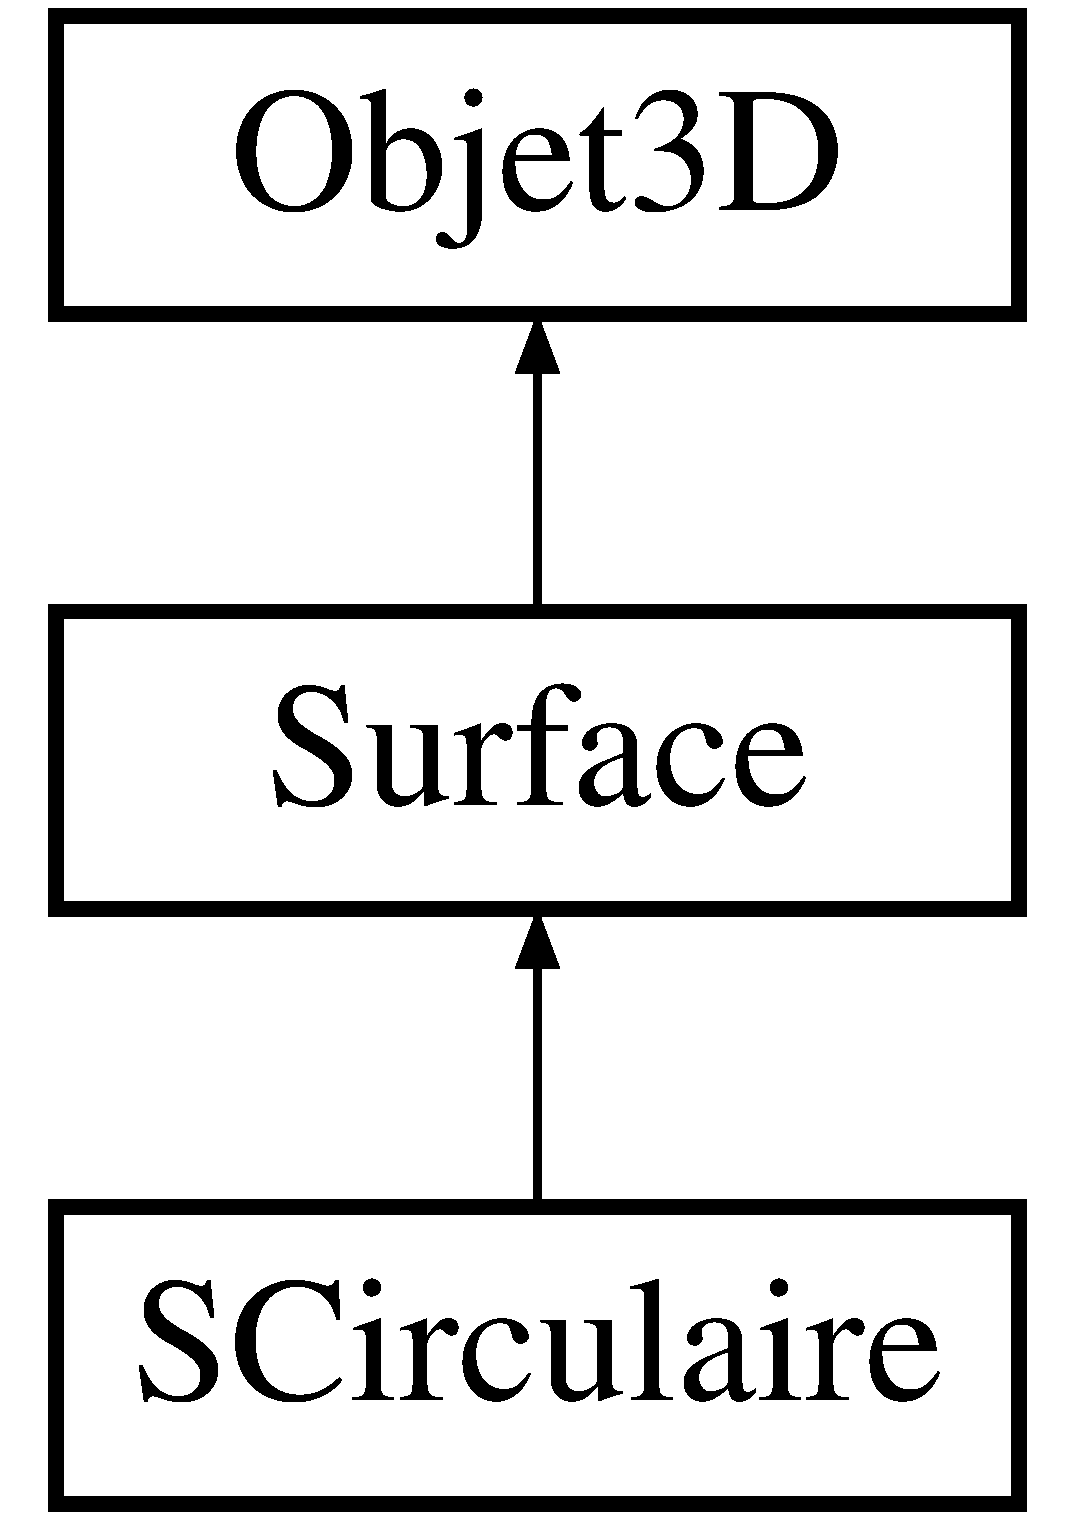
\includegraphics[height=3.000000cm]{classSCirculaire}
\end{center}
\end{figure}
\subsection*{Public Member Functions}
\begin{DoxyCompactItemize}
\item 
\hyperlink{classSCirculaire_abc30b845fc9a038cf3f2d7c3748e2013}{S\-Circulaire} (std\-::vector$<$ \hyperlink{classPointGL}{Point\-G\-L} $\ast$ $>$ c, int n, float rayon)
\begin{DoxyCompactList}\small\item\em Constructeur d'une surface circulaire. \end{DoxyCompactList}\item 
\hypertarget{classSCirculaire_a9cf5f1017dce1bfc41f01562ea57e835}{{\bfseries S\-Circulaire} (const \hyperlink{classSCirculaire}{S\-Circulaire} \&orig)}\label{classSCirculaire_a9cf5f1017dce1bfc41f01562ea57e835}

\item 
\hypertarget{classSCirculaire_aa8cdc58cf4f3c565e9de501552a7b56c}{virtual \hyperlink{classSCirculaire_aa8cdc58cf4f3c565e9de501552a7b56c}{$\sim$\-S\-Circulaire} ()}\label{classSCirculaire_aa8cdc58cf4f3c565e9de501552a7b56c}

\begin{DoxyCompactList}\small\item\em destructeur de la classe qui détruit tous les pointeurs \end{DoxyCompactList}\item 
\hypertarget{classSCirculaire_ab9f9027637a9d0e85061a4d80623fac2}{void \hyperlink{classSCirculaire_ab9f9027637a9d0e85061a4d80623fac2}{Creation} ()}\label{classSCirculaire_ab9f9027637a9d0e85061a4d80623fac2}

\begin{DoxyCompactList}\small\item\em Construction de la surface par ajout des points dans \hyperlink{classSurface}{Surface} L'ajout se fait selon l'ordre suivant\-: Pour chaque points de la courbe on donne tous les points du cercle correspondant au niveau du point de la courbe ($<$=$>$ parallèle par parallèle) méridiens=courbe parallèle=cercle. \end{DoxyCompactList}\item 
void \hyperlink{classSCirculaire_a7db7e11fa18f5e00b870d7c062427572}{construction} ()
\item 
\hypertarget{classSCirculaire_ae1efd417c1a56b007746371e1534a94c}{float {\bfseries Calcul\-Theta} (\hyperlink{classPointGL}{Point\-G\-L} $\ast$p)}\label{classSCirculaire_ae1efd417c1a56b007746371e1534a94c}

\item 
\hypertarget{classSCirculaire_ab7a783cb6bb3e7f9abe1a131503b6292}{float {\bfseries Calcul\-Phi} (\hyperlink{classPointGL}{Point\-G\-L} $\ast$p)}\label{classSCirculaire_ab7a783cb6bb3e7f9abe1a131503b6292}

\item 
\hypertarget{classSCirculaire_a8adc636b41bb85c1340fa98f1c939f56}{std\-::vector$<$ \hyperlink{classFace}{Face} $\ast$ $>$ \hyperlink{classSCirculaire_a8adc636b41bb85c1340fa98f1c939f56}{get\-Face} ()}\label{classSCirculaire_a8adc636b41bb85c1340fa98f1c939f56}

\begin{DoxyCompactList}\small\item\em Fonction permettant l'affichage de la surface. \end{DoxyCompactList}\end{DoxyCompactItemize}
\subsection*{Additional Inherited Members}


\subsection{Detailed Description}
\begin{DoxyAuthor}{Author}
P\-O\-N\-C\-I\-A\-N\-O Jean-\/\-Jacques et P\-R\-U\-D\-H\-O\-M\-M\-E Claire 
\end{DoxyAuthor}
\begin{DoxyDate}{Date}
13/03/2014
\end{DoxyDate}
Cette oeuvre, création, code, site ou texte est sous licence Creative Commons Attribution -\/ Pas d’\-Utilisation Commerciale -\/ Partage dans les Mêmes Conditions 4.\-0 International. Pour accéder à une copie de cette licence, merci de vous rendre à l'adresse suivante \href{http://creativecommons.org/licenses/by-nc-sa/4.0/deed.fr}{\tt http\-://creativecommons.\-org/licenses/by-\/nc-\/sa/4.\-0/deed.\-fr} ou envoyez un courrier à Creative Commons, 444 Castro Street, Suite 900, Mountain View, California, 94041, U\-S\-A. Copyright 2014

Contact\-: \href{mailto:ponciano.jeanjacques@gmail.com}{\tt ponciano.\-jeanjacques@gmail.\-com} 

\subsection{Constructor \& Destructor Documentation}
\hypertarget{classSCirculaire_abc30b845fc9a038cf3f2d7c3748e2013}{\index{S\-Circulaire@{S\-Circulaire}!S\-Circulaire@{S\-Circulaire}}
\index{S\-Circulaire@{S\-Circulaire}!SCirculaire@{S\-Circulaire}}
\subsubsection[{S\-Circulaire}]{\setlength{\rightskip}{0pt plus 5cm}S\-Circulaire\-::\-S\-Circulaire (
\begin{DoxyParamCaption}
\item[{std\-::vector$<$ {\bf Point\-G\-L} $\ast$ $>$}]{c, }
\item[{int}]{n, }
\item[{float}]{rayon}
\end{DoxyParamCaption}
)}}\label{classSCirculaire_abc30b845fc9a038cf3f2d7c3748e2013}


Constructeur d'une surface circulaire. 


\begin{DoxyParams}{Parameters}
{\em c} & vecteur de points correspondant au points appartenant à la courbe de référence sur laquelle repose la surface. Exemple\-: 
\begin{DoxyCode}
\hyperlink{classBezier}{Bezier}* b=\textcolor{keyword}{new} \hyperlink{classBezier}{Bezier}(10);
b->\hyperlink{classBezier_a3973f77432e3a02a7971d6a524668aef}{Trace}(vectorPtsControleC, nbp);
\hyperlink{classSCirculaire}{SCirculaire}* sl=\textcolor{keyword}{new} \hyperlink{classSCirculaire_abc30b845fc9a038cf3f2d7c3748e2013}{SCirculaire}(b.\hyperlink{classBezier_ac428660e18d25b27a4e60b911c10320e}{getP}(), nbp2, centre);
\end{DoxyCode}
 \\
\hline
{\em n} & nombre de méridien pour la surface \\
\hline
{\em centre} & est le centre de la rotation effectuée par la courbe pour créer la surface \\
\hline
\end{DoxyParams}


\subsection{Member Function Documentation}
\hypertarget{classSCirculaire_a7db7e11fa18f5e00b870d7c062427572}{\index{S\-Circulaire@{S\-Circulaire}!construction@{construction}}
\index{construction@{construction}!SCirculaire@{S\-Circulaire}}
\subsubsection[{construction}]{\setlength{\rightskip}{0pt plus 5cm}void S\-Circulaire\-::construction (
\begin{DoxyParamCaption}
{}
\end{DoxyParamCaption}
)\hspace{0.3cm}{\ttfamily [virtual]}}}\label{classSCirculaire_a7db7e11fa18f5e00b870d7c062427572}
Calcule tous les points de l'objet 

Reimplemented from \hyperlink{classObjet3D_adeb89dbb10335cd671378377818c1f71}{Objet3\-D}.



The documentation for this class was generated from the following files\-:\begin{DoxyCompactItemize}
\item 
modules/open\-G\-L/tools\-\_\-models/\-Surfaces/S\-Circulaire.\-h\item 
modules/open\-G\-L/tools\-\_\-models/\-Surfaces/S\-Circulaire.\-cpp\end{DoxyCompactItemize}

\hypertarget{classScnData}{\section{Scn\-Data Class Reference}
\label{classScnData}\index{Scn\-Data@{Scn\-Data}}
}
\subsection*{Public Member Functions}
\begin{DoxyCompactItemize}
\item 
\hypertarget{classScnData_a56a78467b0952f1059a39a882465fd6d}{{\bfseries Scn\-Data} (std\-::string pathname)}\label{classScnData_a56a78467b0952f1059a39a882465fd6d}

\item 
void \hyperlink{classScnData_ad38f540cf59168597be7e9ecf32a4901}{load\-From\-S\-C\-N} (std\-::string pathname)
\begin{DoxyCompactList}\small\item\em load\-From\-S\-C\-N \end{DoxyCompactList}\item 
\hypertarget{classScnData_a4a8fe4672185846fb4f6e6ad6ac62eef}{Q\-Vector$<$ \hyperlink{classDatapackage}{Datapackage} $>$ {\bfseries get\-Packages} () const }\label{classScnData_a4a8fe4672185846fb4f6e6ad6ac62eef}

\item 
\hypertarget{classScnData_a8bbb0728d350e8fa6f55dc66f6de2d23}{void {\bfseries set\-Packages} (const Q\-Vector$<$ \hyperlink{classDatapackage}{Datapackage} $>$ \&value)}\label{classScnData_a8bbb0728d350e8fa6f55dc66f6de2d23}

\item 
\hypertarget{classScnData_aa3ec98a431ba09c271b63591a698527e}{Q\-Byte\-Array {\bfseries get\-Alldatas} () const }\label{classScnData_aa3ec98a431ba09c271b63591a698527e}

\item 
\hypertarget{classScnData_a071d7a5a8cb03dc7ef796a1b24eb1d6a}{void {\bfseries set\-Alldatas} (const Q\-Byte\-Array \&value)}\label{classScnData_a071d7a5a8cb03dc7ef796a1b24eb1d6a}

\item 
\hypertarget{classScnData_ac89256a37f64c12026b872a0e3837f70}{int {\bfseries get\-Indexreader} () const }\label{classScnData_ac89256a37f64c12026b872a0e3837f70}

\item 
\hypertarget{classScnData_a6af731fe1cbda4d1d49db4b2fad27073}{void {\bfseries set\-Indexreader} (int value)}\label{classScnData_a6af731fe1cbda4d1d49db4b2fad27073}

\end{DoxyCompactItemize}


\subsection{Member Function Documentation}
\hypertarget{classScnData_ad38f540cf59168597be7e9ecf32a4901}{\index{Scn\-Data@{Scn\-Data}!load\-From\-S\-C\-N@{load\-From\-S\-C\-N}}
\index{load\-From\-S\-C\-N@{load\-From\-S\-C\-N}!ScnData@{Scn\-Data}}
\subsubsection[{load\-From\-S\-C\-N}]{\setlength{\rightskip}{0pt plus 5cm}void Scn\-Data\-::load\-From\-S\-C\-N (
\begin{DoxyParamCaption}
\item[{std\-::string}]{pathname}
\end{DoxyParamCaption}
)}}\label{classScnData_ad38f540cf59168597be7e9ecf32a4901}


load\-From\-S\-C\-N 


\begin{DoxyParams}{Parameters}
{\em pathname} & the path of the load file \\
\hline
\end{DoxyParams}
\begin{DoxyReturn}{Returns}
the cloud loaded 
\end{DoxyReturn}


The documentation for this class was generated from the following files\-:\begin{DoxyCompactItemize}
\item 
works/scndata.\-h\item 
works/scndata.\-cpp\end{DoxyCompactItemize}

\hypertarget{classscnreader__model}{\section{scnreader\-\_\-model Class Reference}
\label{classscnreader__model}\index{scnreader\-\_\-model@{scnreader\-\_\-model}}
}
Inheritance diagram for scnreader\-\_\-model\-:\begin{figure}[H]
\begin{center}
\leavevmode
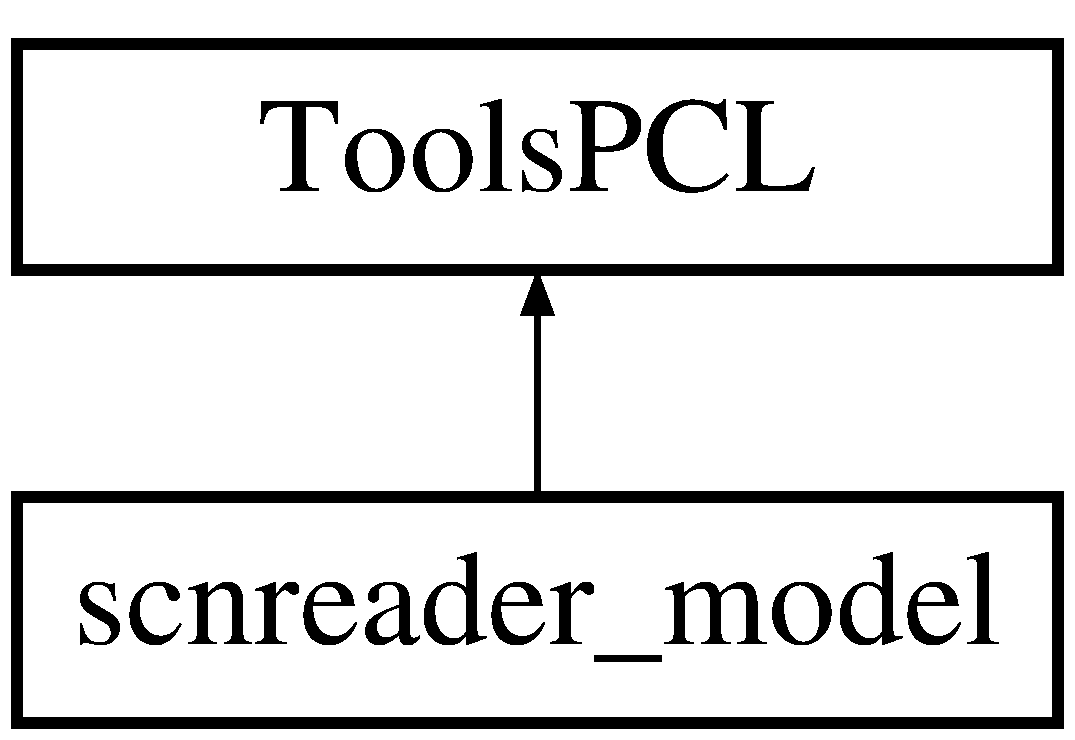
\includegraphics[height=2.000000cm]{classscnreader__model}
\end{center}
\end{figure}
\subsection*{Public Member Functions}
\begin{DoxyCompactItemize}
\item 
void \hyperlink{classscnreader__model_ad40c19b946f2299d290adc7c4acc9a13}{load\-From\-S\-C\-N} (std\-::string pathname)
\begin{DoxyCompactList}\small\item\em \hyperlink{classscnreader__model_ad40c19b946f2299d290adc7c4acc9a13}{scnreader\-\_\-model\-::load\-From\-S\-C\-N} create and add data from file \end{DoxyCompactList}\item 
\hypertarget{classscnreader__model_a6c2fae26489c9f8b43aca8775413732d}{\hyperlink{classScnData}{Scn\-Data} {\bfseries get\-Data} (int i) const }\label{classscnreader__model_a6c2fae26489c9f8b43aca8775413732d}

\item 
\hypertarget{classscnreader__model_a5371eaafd61ea9b18d04ac11e5e03218}{void {\bfseries set\-Datas} (const Q\-Vector$<$ \hyperlink{classScnData}{Scn\-Data} $>$ \&value)}\label{classscnreader__model_a5371eaafd61ea9b18d04ac11e5e03218}

\end{DoxyCompactItemize}
\subsection*{Additional Inherited Members}


\subsection{Member Function Documentation}
\hypertarget{classscnreader__model_ad40c19b946f2299d290adc7c4acc9a13}{\index{scnreader\-\_\-model@{scnreader\-\_\-model}!load\-From\-S\-C\-N@{load\-From\-S\-C\-N}}
\index{load\-From\-S\-C\-N@{load\-From\-S\-C\-N}!scnreader_model@{scnreader\-\_\-model}}
\subsubsection[{load\-From\-S\-C\-N}]{\setlength{\rightskip}{0pt plus 5cm}void scnreader\-\_\-model\-::load\-From\-S\-C\-N (
\begin{DoxyParamCaption}
\item[{std\-::string}]{pathname}
\end{DoxyParamCaption}
)}}\label{classscnreader__model_ad40c19b946f2299d290adc7c4acc9a13}


\hyperlink{classscnreader__model_ad40c19b946f2299d290adc7c4acc9a13}{scnreader\-\_\-model\-::load\-From\-S\-C\-N} create and add data from file 


\begin{DoxyParams}{Parameters}
{\em pathname} & the file in svn format \\
\hline
\end{DoxyParams}


The documentation for this class was generated from the following files\-:\begin{DoxyCompactItemize}
\item 
works/scnreader\-\_\-model.\-h\item 
works/scnreader\-\_\-model.\-cpp\end{DoxyCompactItemize}

\hypertarget{classscnreader__view}{\section{scnreader\-\_\-view Class Reference}
\label{classscnreader__view}\index{scnreader\-\_\-view@{scnreader\-\_\-view}}
}
Inheritance diagram for scnreader\-\_\-view\-:\begin{figure}[H]
\begin{center}
\leavevmode
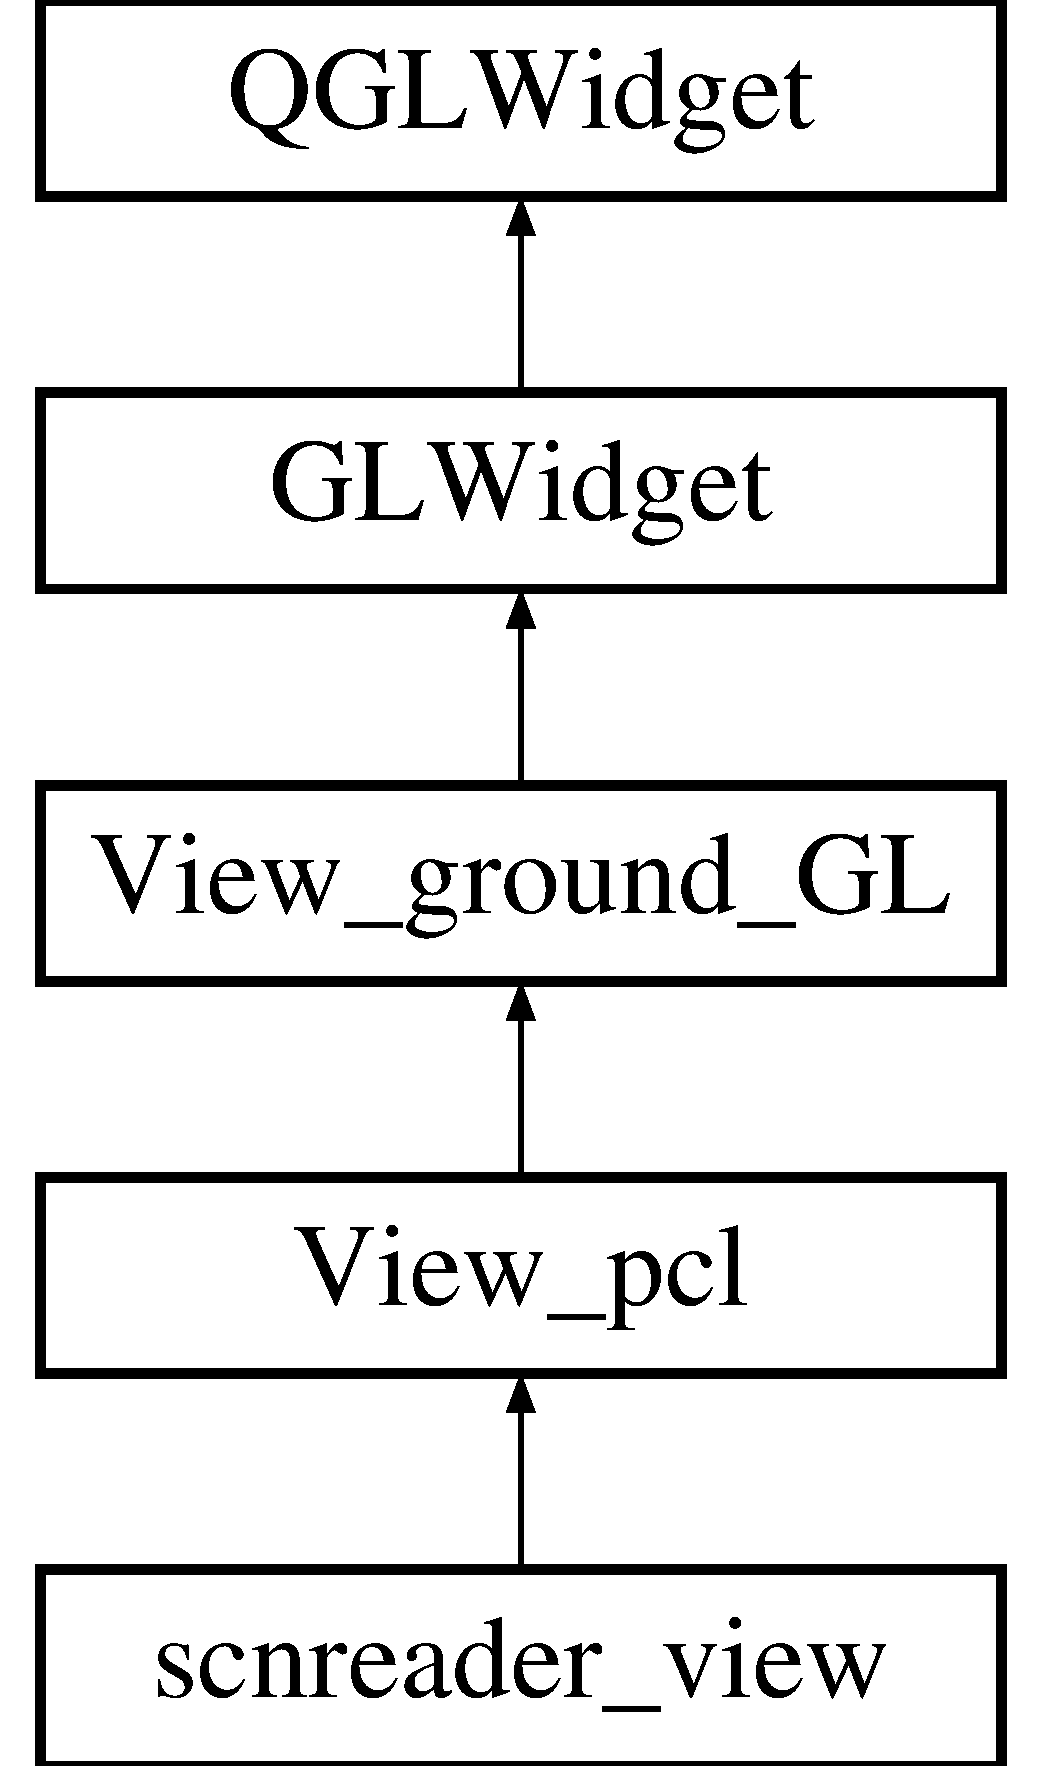
\includegraphics[height=5.000000cm]{classscnreader__view}
\end{center}
\end{figure}
\subsection*{Public Member Functions}
\begin{DoxyCompactItemize}
\item 
\hypertarget{classscnreader__view_a3b20e7436fedcf438de209200005b974}{{\bfseries scnreader\-\_\-view} (Q\-Widget $\ast$parent=0)}\label{classscnreader__view_a3b20e7436fedcf438de209200005b974}

\item 
\hypertarget{classscnreader__view_a977fd9239e1cf795da0d1720b8e192d1}{void {\bfseries paint\-G\-L} ()}\label{classscnreader__view_a977fd9239e1cf795da0d1720b8e192d1}

\item 
\hypertarget{classscnreader__view_a108b2d99a8fb80d1f7b89cf3a81ddc30}{void {\bfseries load\-From\-S\-C\-N} ()}\label{classscnreader__view_a108b2d99a8fb80d1f7b89cf3a81ddc30}

\end{DoxyCompactItemize}
\subsection*{Additional Inherited Members}


The documentation for this class was generated from the following files\-:\begin{DoxyCompactItemize}
\item 
works/scnreader\-\_\-view.\-h\item 
works/scnreader\-\_\-view.\-cpp\end{DoxyCompactItemize}

\hypertarget{classSLineaire}{\section{S\-Lineaire Class Reference}
\label{classSLineaire}\index{S\-Lineaire@{S\-Lineaire}}
}


{\ttfamily \#include $<$S\-Lineaire.\-h$>$}

Inheritance diagram for S\-Lineaire\-:\begin{figure}[H]
\begin{center}
\leavevmode
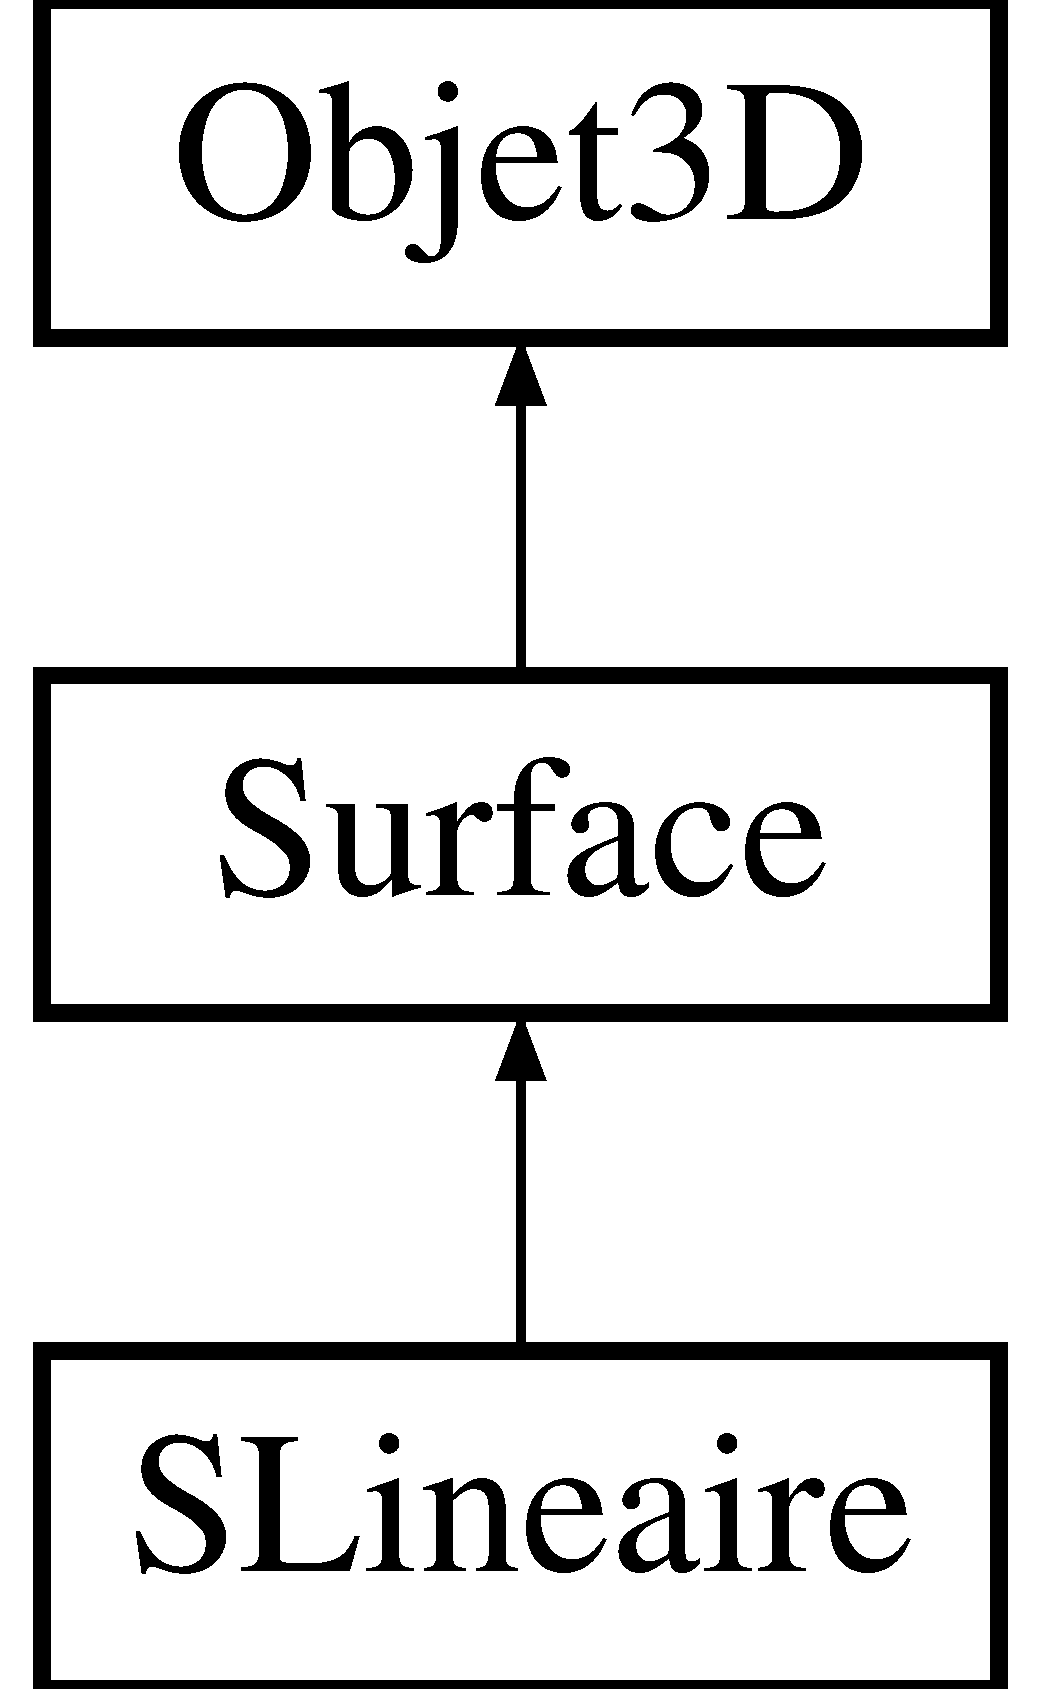
\includegraphics[height=3.000000cm]{classSLineaire}
\end{center}
\end{figure}
\subsection*{Public Member Functions}
\begin{DoxyCompactItemize}
\item 
\hyperlink{classSLineaire_af29a55c43b2f69187e9bf7d2f01e3199}{S\-Lineaire} (std\-::vector$<$ \hyperlink{classPointGL}{Point\-G\-L} $\ast$ $>$ c, int n, \hyperlink{classPointGL}{Point\-G\-L} $\ast$p1, \hyperlink{classPointGL}{Point\-G\-L} $\ast$p2)
\begin{DoxyCompactList}\small\item\em Constructeur d'une surface linéaire. \end{DoxyCompactList}\item 
\hypertarget{classSLineaire_a99e6bd4a84347cffba0f3f5fcda2f228}{{\bfseries S\-Lineaire} (const \hyperlink{classSLineaire}{S\-Lineaire} \&orig)}\label{classSLineaire_a99e6bd4a84347cffba0f3f5fcda2f228}

\item 
\hypertarget{classSLineaire_a85d96a0221719b0397625f99dcb9d964}{virtual \hyperlink{classSLineaire_a85d96a0221719b0397625f99dcb9d964}{$\sim$\-S\-Lineaire} ()}\label{classSLineaire_a85d96a0221719b0397625f99dcb9d964}

\begin{DoxyCompactList}\small\item\em destructeur de la classe qui détruit tous les pointeurs \end{DoxyCompactList}\item 
\hypertarget{classSLineaire_a946fddfdae938c4d3ec6e91c9cb30b8c}{void \hyperlink{classSLineaire_a946fddfdae938c4d3ec6e91c9cb30b8c}{Creation} ()}\label{classSLineaire_a946fddfdae938c4d3ec6e91c9cb30b8c}

\begin{DoxyCompactList}\small\item\em Construction de la surface par ajout des points dans \hyperlink{classSurface}{Surface} L'ajout se fait selon l'ordre suivant\-: Pour chaque points de la courbe on donne tous les points du segment qui a pour origine le point de la courbe ($<$=$>$ parallèle par parallèle) méridiens=courbe parallèle=segment. \end{DoxyCompactList}\item 
\hypertarget{classSLineaire_a3c82b3b19ad80e6815ca86cbb23facb9}{void \hyperlink{classSLineaire_a3c82b3b19ad80e6815ca86cbb23facb9}{construction} ()}\label{classSLineaire_a3c82b3b19ad80e6815ca86cbb23facb9}

\begin{DoxyCompactList}\small\item\em Fonction permettant l'affichage de la surface. \end{DoxyCompactList}\item 
float \hyperlink{classSLineaire_aa50f3a000493441aa2ace64806e1ae9d}{Interpo\-Lineaire} (float t, float p0, float p1)
\begin{DoxyCompactList}\small\item\em Fonction permettant de calculer l'interpolation linéaire entre p0 et p1 à l'instant t. \end{DoxyCompactList}\end{DoxyCompactItemize}
\subsection*{Additional Inherited Members}


\subsection{Detailed Description}
\begin{DoxyAuthor}{Author}
P\-O\-N\-C\-I\-A\-N\-O Jean-\/\-Jacques et P\-R\-U\-D\-H\-O\-M\-M\-E Claire 
\end{DoxyAuthor}
\begin{DoxyDate}{Date}
13/03/2014
\end{DoxyDate}
Cette oeuvre, création, code, site ou texte est sous licence Creative Commons Attribution -\/ Pas d’\-Utilisation Commerciale -\/ Partage dans les Mêmes Conditions 4.\-0 International. Pour accéder à une copie de cette licence, merci de vous rendre à l'adresse suivante \href{http://creativecommons.org/licenses/by-nc-sa/4.0/deed.fr}{\tt http\-://creativecommons.\-org/licenses/by-\/nc-\/sa/4.\-0/deed.\-fr} ou envoyez un courrier à Creative Commons, 444 Castro Street, Suite 900, Mountain View, California, 94041, U\-S\-A. Copyright 2014

Contact\-: \href{mailto:ponciano.jeanjacques@gmail.com}{\tt ponciano.\-jeanjacques@gmail.\-com} 

\subsection{Constructor \& Destructor Documentation}
\hypertarget{classSLineaire_af29a55c43b2f69187e9bf7d2f01e3199}{\index{S\-Lineaire@{S\-Lineaire}!S\-Lineaire@{S\-Lineaire}}
\index{S\-Lineaire@{S\-Lineaire}!SLineaire@{S\-Lineaire}}
\subsubsection[{S\-Lineaire}]{\setlength{\rightskip}{0pt plus 5cm}S\-Lineaire\-::\-S\-Lineaire (
\begin{DoxyParamCaption}
\item[{std\-::vector$<$ {\bf Point\-G\-L} $\ast$ $>$}]{c, }
\item[{int}]{n, }
\item[{{\bf Point\-G\-L} $\ast$}]{p1, }
\item[{{\bf Point\-G\-L} $\ast$}]{p2}
\end{DoxyParamCaption}
)}}\label{classSLineaire_af29a55c43b2f69187e9bf7d2f01e3199}


Constructeur d'une surface linéaire. 


\begin{DoxyParams}{Parameters}
{\em c} & vecteur de points correspondant au points appartenant à la courbe de référence sur laquelle repose la surface. Exemple\-: 
\begin{DoxyCode}
\hyperlink{classBezier}{Bezier}* b=\textcolor{keyword}{new} \hyperlink{classBezier}{Bezier}(10);
b->\hyperlink{classBezier_a3973f77432e3a02a7971d6a524668aef}{Trace}(vectorPtsControleC, nbp);
\hyperlink{classSLineaire}{SLineaire}* sl=\textcolor{keyword}{new} \hyperlink{classSLineaire_af29a55c43b2f69187e9bf7d2f01e3199}{SLineaire}(b.\hyperlink{classBezier_ac428660e18d25b27a4e60b911c10320e}{getP}(), nbp2, p1, p2);
\end{DoxyCode}
 \\
\hline
{\em n} & nombre de méridien pour la surface \\
\hline
{\em p1} & premier point du segment \mbox{[}p1,p2\mbox{]} permettant la construction linéaire le long de la courbe \\
\hline
{\em p2} & second point du segment \mbox{[}p1,p2\mbox{]} permettant la construction linéaire le long de la courbe Le segment \mbox{[}p1,p2\mbox{]} est le segment que l'on balade le long de la courbe pour obtenir la surface \\
\hline
\end{DoxyParams}


\subsection{Member Function Documentation}
\hypertarget{classSLineaire_aa50f3a000493441aa2ace64806e1ae9d}{\index{S\-Lineaire@{S\-Lineaire}!Interpo\-Lineaire@{Interpo\-Lineaire}}
\index{Interpo\-Lineaire@{Interpo\-Lineaire}!SLineaire@{S\-Lineaire}}
\subsubsection[{Interpo\-Lineaire}]{\setlength{\rightskip}{0pt plus 5cm}float S\-Lineaire\-::\-Interpo\-Lineaire (
\begin{DoxyParamCaption}
\item[{float}]{t, }
\item[{float}]{p0, }
\item[{float}]{p1}
\end{DoxyParamCaption}
)}}\label{classSLineaire_aa50f3a000493441aa2ace64806e1ae9d}


Fonction permettant de calculer l'interpolation linéaire entre p0 et p1 à l'instant t. 


\begin{DoxyParams}{Parameters}
{\em t} & instant/avancement de l'interpolation linéaire \\
\hline
{\em p0} & point de départ de l'interpolation linéaire \\
\hline
{\em p1} & point d'arrivée de l'interpolation linéaire \\
\hline
\end{DoxyParams}
\begin{DoxyReturn}{Returns}
la valeur correspondant à l'interpolation linéaire entre p0 et p1 à l'instant t 
\end{DoxyReturn}


The documentation for this class was generated from the following files\-:\begin{DoxyCompactItemize}
\item 
modules/open\-G\-L/tools\-\_\-models/\-Surfaces/S\-Lineaire.\-h\item 
modules/open\-G\-L/tools\-\_\-models/\-Surfaces/S\-Lineaire.\-cpp\end{DoxyCompactItemize}

\hypertarget{classSphere}{\section{Sphere Class Reference}
\label{classSphere}\index{Sphere@{Sphere}}
}


{\ttfamily \#include $<$Sphere.\-h$>$}

Inheritance diagram for Sphere\-:\begin{figure}[H]
\begin{center}
\leavevmode
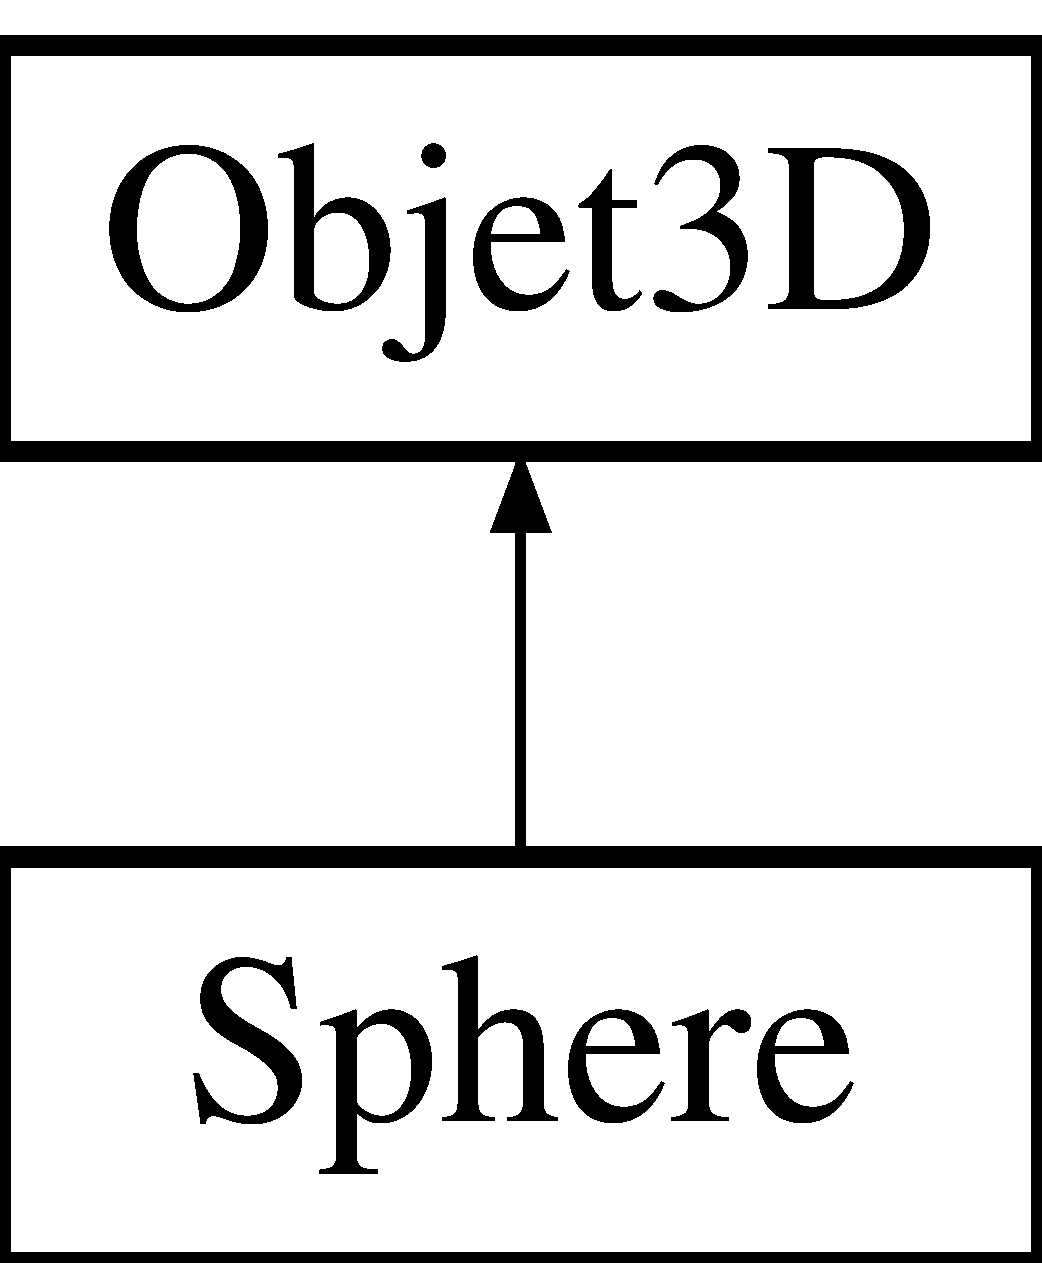
\includegraphics[height=2.000000cm]{classSphere}
\end{center}
\end{figure}
\subsection*{Public Member Functions}
\begin{DoxyCompactItemize}
\item 
\hypertarget{classSphere_ae9f149be4c2fd7ad78488cdd237ba560}{{\bfseries Sphere} (float r, int parallele, int meridien)}\label{classSphere_ae9f149be4c2fd7ad78488cdd237ba560}

\item 
\hypertarget{classSphere_a20d301e4c5016a72b6dbcdcaf38c839b}{{\bfseries Sphere} (const \hyperlink{classSphere}{Sphere} \&orig)}\label{classSphere_a20d301e4c5016a72b6dbcdcaf38c839b}

\item 
void \hyperlink{classSphere_a60631bd7158f7c443ebc5bda6066d2a2}{construction} ()
\item 
void \hyperlink{classSphere_ae0e7a735e87a6e90562bec0d887de08c}{set\-Couleur} (float r, float g, float b)
\item 
void \hyperlink{classSphere_a5a859a0055c250295ef6b13b662d9e76}{set\-Couleur} (const \hyperlink{classCouleur}{Couleur} \&c)
\item 
void \hyperlink{classSphere_ad39d66f77eb545c05f16b51539c80269}{affiche\-Points} ()
\item 
void \hyperlink{classSphere_a58ba7340a42539ffd726413e2a3178a3}{affichage} ()
\end{DoxyCompactItemize}
\subsection*{Additional Inherited Members}


\subsection{Detailed Description}
\begin{DoxyAuthor}{Author}
P\-O\-N\-C\-I\-A\-N\-O Jean-\/\-Jacques et P\-R\-U\-D\-H\-O\-M\-M\-E Claire 
\end{DoxyAuthor}
\begin{DoxyDate}{Date}
13/03/2014
\end{DoxyDate}
Cette oeuvre, création, code, site ou texte est sous licence Creative Commons Attribution -\/ Pas d’\-Utilisation Commerciale -\/ Partage dans les Mêmes Conditions 4.\-0 International. Pour accéder à une copie de cette licence, merci de vous rendre à l'adresse suivante \href{http://creativecommons.org/licenses/by-nc-sa/4.0/deed.fr}{\tt http\-://creativecommons.\-org/licenses/by-\/nc-\/sa/4.\-0/deed.\-fr} ou envoyez un courrier à Creative Commons, 444 Castro Street, Suite 900, Mountain View, California, 94041, U\-S\-A. Copyright 2014

Contact\-: \href{mailto:ponciano.jeanjacques@gmail.com}{\tt ponciano.\-jeanjacques@gmail.\-com} 

\subsection{Member Function Documentation}
\hypertarget{classSphere_a58ba7340a42539ffd726413e2a3178a3}{\index{Sphere@{Sphere}!affichage@{affichage}}
\index{affichage@{affichage}!Sphere@{Sphere}}
\subsubsection[{affichage}]{\setlength{\rightskip}{0pt plus 5cm}void Sphere\-::affichage (
\begin{DoxyParamCaption}
{}
\end{DoxyParamCaption}
)}}\label{classSphere_a58ba7340a42539ffd726413e2a3178a3}
Affiche l'objet \hypertarget{classSphere_ad39d66f77eb545c05f16b51539c80269}{\index{Sphere@{Sphere}!affiche\-Points@{affiche\-Points}}
\index{affiche\-Points@{affiche\-Points}!Sphere@{Sphere}}
\subsubsection[{affiche\-Points}]{\setlength{\rightskip}{0pt plus 5cm}void Sphere\-::affiche\-Points (
\begin{DoxyParamCaption}
{}
\end{DoxyParamCaption}
)}}\label{classSphere_ad39d66f77eb545c05f16b51539c80269}
Affiche chaque point de la sphere \hypertarget{classSphere_a60631bd7158f7c443ebc5bda6066d2a2}{\index{Sphere@{Sphere}!construction@{construction}}
\index{construction@{construction}!Sphere@{Sphere}}
\subsubsection[{construction}]{\setlength{\rightskip}{0pt plus 5cm}void Sphere\-::construction (
\begin{DoxyParamCaption}
{}
\end{DoxyParamCaption}
)\hspace{0.3cm}{\ttfamily [virtual]}}}\label{classSphere_a60631bd7158f7c443ebc5bda6066d2a2}
Calcule tous les points de la sphere 

Reimplemented from \hyperlink{classObjet3D_adeb89dbb10335cd671378377818c1f71}{Objet3\-D}.

\hypertarget{classSphere_ae0e7a735e87a6e90562bec0d887de08c}{\index{Sphere@{Sphere}!set\-Couleur@{set\-Couleur}}
\index{set\-Couleur@{set\-Couleur}!Sphere@{Sphere}}
\subsubsection[{set\-Couleur}]{\setlength{\rightskip}{0pt plus 5cm}void Sphere\-::set\-Couleur (
\begin{DoxyParamCaption}
\item[{float}]{r, }
\item[{float}]{g, }
\item[{float}]{b}
\end{DoxyParamCaption}
)}}\label{classSphere_ae0e7a735e87a6e90562bec0d887de08c}
Affecte une couleur aux faces 
\begin{DoxyParams}{Parameters}
{\em r} & canal rouge \\
\hline
{\em g} & canal vert \\
\hline
{\em b} & canal bleu \\
\hline
\end{DoxyParams}
\hypertarget{classSphere_a5a859a0055c250295ef6b13b662d9e76}{\index{Sphere@{Sphere}!set\-Couleur@{set\-Couleur}}
\index{set\-Couleur@{set\-Couleur}!Sphere@{Sphere}}
\subsubsection[{set\-Couleur}]{\setlength{\rightskip}{0pt plus 5cm}void Sphere\-::set\-Couleur (
\begin{DoxyParamCaption}
\item[{const {\bf Couleur} \&}]{c}
\end{DoxyParamCaption}
)}}\label{classSphere_a5a859a0055c250295ef6b13b662d9e76}
Affecte une couleur aux faces 
\begin{DoxyParams}{Parameters}
{\em c} & couleur \\
\hline
\end{DoxyParams}


The documentation for this class was generated from the following files\-:\begin{DoxyCompactItemize}
\item 
modules/open\-G\-L/tools\-\_\-models/objets/Sphere.\-h\item 
modules/open\-G\-L/tools\-\_\-models/objets/Sphere.\-cpp\end{DoxyCompactItemize}

\hypertarget{classSRevolution}{\section{S\-Revolution Class Reference}
\label{classSRevolution}\index{S\-Revolution@{S\-Revolution}}
}


{\ttfamily \#include $<$S\-Revolution.\-h$>$}

Inheritance diagram for S\-Revolution\-:\begin{figure}[H]
\begin{center}
\leavevmode
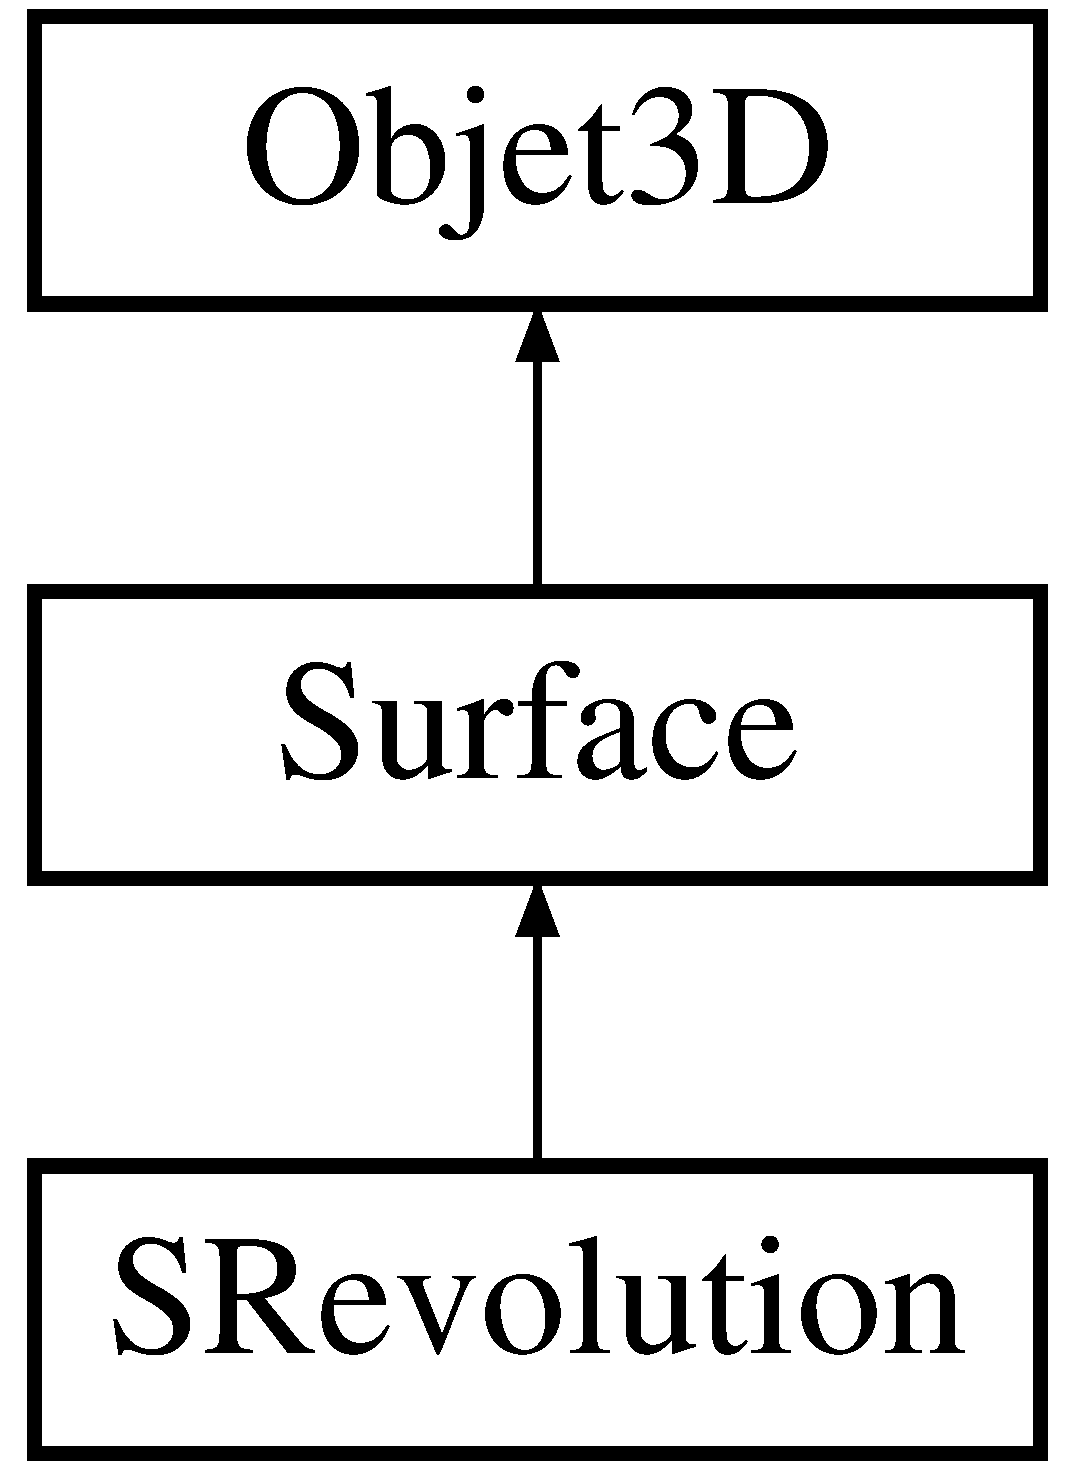
\includegraphics[height=3.000000cm]{classSRevolution}
\end{center}
\end{figure}
\subsection*{Public Member Functions}
\begin{DoxyCompactItemize}
\item 
\hyperlink{classSRevolution_a57a7215ff953ee4f6ec1ccb8d330b087}{S\-Revolution} (std\-::vector$<$ \hyperlink{classPointGL}{Point\-G\-L} $\ast$ $>$ c, int n)
\begin{DoxyCompactList}\small\item\em Constructeur d'une surface de révolution. \end{DoxyCompactList}\item 
\hypertarget{classSRevolution_a846beb4fa33dc09ce2d6cf49ee843960}{{\bfseries S\-Revolution} (const \hyperlink{classSRevolution}{S\-Revolution} \&orig)}\label{classSRevolution_a846beb4fa33dc09ce2d6cf49ee843960}

\item 
\hypertarget{classSRevolution_ae78dddc5cd493f71796b4ac21b840e9f}{virtual \hyperlink{classSRevolution_ae78dddc5cd493f71796b4ac21b840e9f}{$\sim$\-S\-Revolution} ()}\label{classSRevolution_ae78dddc5cd493f71796b4ac21b840e9f}

\begin{DoxyCompactList}\small\item\em destructeur de la classe qui détruit tous les pointeurs \end{DoxyCompactList}\item 
\hypertarget{classSRevolution_af42d610f9cd60bf946ff032d5d02d203}{void \hyperlink{classSRevolution_af42d610f9cd60bf946ff032d5d02d203}{creation} ()}\label{classSRevolution_af42d610f9cd60bf946ff032d5d02d203}

\begin{DoxyCompactList}\small\item\em Construction de la surface par ajout des points dans \hyperlink{classSurface}{Surface} L'ajout se fait selon l'ordre suivant\-: Pour chaque points de la courbe on donne tous les points du cercle correspondant au niveau du point de la courbe ($<$=$>$ parallèle par parallèle) méridiens=courbe parallèle=cercle. \end{DoxyCompactList}\end{DoxyCompactItemize}
\subsection*{Additional Inherited Members}


\subsection{Detailed Description}
\begin{DoxyAuthor}{Author}
P\-O\-N\-C\-I\-A\-N\-O Jean-\/\-Jacques et P\-R\-U\-D\-H\-O\-M\-M\-E Claire 
\end{DoxyAuthor}
\begin{DoxyDate}{Date}
13/03/2014
\end{DoxyDate}
Cette oeuvre, création, code, site ou texte est sous licence Creative Commons Attribution -\/ Pas d’\-Utilisation Commerciale -\/ Partage dans les Mêmes Conditions 4.\-0 International. Pour accéder à une copie de cette licence, merci de vous rendre à l'adresse suivante \href{http://creativecommons.org/licenses/by-nc-sa/4.0/deed.fr}{\tt http\-://creativecommons.\-org/licenses/by-\/nc-\/sa/4.\-0/deed.\-fr} ou envoyez un courrier à Creative Commons, 444 Castro Street, Suite 900, Mountain View, California, 94041, U\-S\-A. Copyright 2014

Contact\-: \href{mailto:ponciano.jeanjacques@gmail.com}{\tt ponciano.\-jeanjacques@gmail.\-com} 

\subsection{Constructor \& Destructor Documentation}
\hypertarget{classSRevolution_a57a7215ff953ee4f6ec1ccb8d330b087}{\index{S\-Revolution@{S\-Revolution}!S\-Revolution@{S\-Revolution}}
\index{S\-Revolution@{S\-Revolution}!SRevolution@{S\-Revolution}}
\subsubsection[{S\-Revolution}]{\setlength{\rightskip}{0pt plus 5cm}S\-Revolution\-::\-S\-Revolution (
\begin{DoxyParamCaption}
\item[{std\-::vector$<$ {\bf Point\-G\-L} $\ast$ $>$}]{c, }
\item[{int}]{n}
\end{DoxyParamCaption}
)}}\label{classSRevolution_a57a7215ff953ee4f6ec1ccb8d330b087}


Constructeur d'une surface de révolution. 


\begin{DoxyParams}{Parameters}
{\em c} & vecteur de points correspondant au points appartenant à la courbe de référence sur laquelle repose la surface. Exemple\-: 
\begin{DoxyCode}
\hyperlink{classBezier}{Bezier}* b=\textcolor{keyword}{new} \hyperlink{classBezier}{Bezier}(10);
b->\hyperlink{classBezier_a3973f77432e3a02a7971d6a524668aef}{Trace}(vectorPtsControleC, nbp);
\hyperlink{classSRevolution}{SRevolution}* sl=\textcolor{keyword}{new} \hyperlink{classSRevolution_a57a7215ff953ee4f6ec1ccb8d330b087}{SRevolution}(b.\hyperlink{classBezier_ac428660e18d25b27a4e60b911c10320e}{getP}(), nbp2);
\end{DoxyCode}
 \\
\hline
{\em n} & nombre de méridien pour la surface \\
\hline
\end{DoxyParams}


The documentation for this class was generated from the following files\-:\begin{DoxyCompactItemize}
\item 
modules/open\-G\-L/tools\-\_\-models/\-Surfaces/S\-Revolution.\-h\item 
modules/open\-G\-L/tools\-\_\-models/\-Surfaces/S\-Revolution.\-cpp\end{DoxyCompactItemize}

\hypertarget{classSurface}{\section{Surface Class Reference}
\label{classSurface}\index{Surface@{Surface}}
}


{\ttfamily \#include $<$Surface.\-h$>$}

Inheritance diagram for Surface\-:\begin{figure}[H]
\begin{center}
\leavevmode
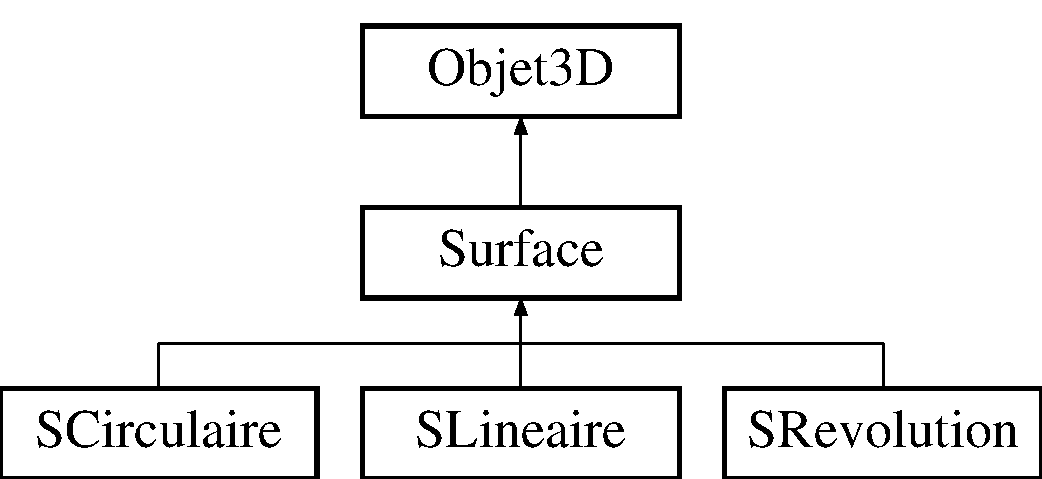
\includegraphics[height=3.000000cm]{classSurface}
\end{center}
\end{figure}
\subsection*{Public Member Functions}
\begin{DoxyCompactItemize}
\item 
\hyperlink{classSurface_ade400cdb9710332c4b0902fc8c385376}{Surface} (std\-::vector$<$ \hyperlink{classPointGL}{Point\-G\-L} $\ast$ $>$ c, int n)
\begin{DoxyCompactList}\small\item\em Constructeur d'une surface. \end{DoxyCompactList}\item 
\hypertarget{classSurface_a81c20bc2a06703270cd283cecb27580b}{{\bfseries Surface} (const \hyperlink{classSurface}{Surface} \&orig)}\label{classSurface_a81c20bc2a06703270cd283cecb27580b}

\item 
\hypertarget{classSurface_a89de75c95cb550d432f3ea4ed1429db0}{virtual \hyperlink{classSurface_a89de75c95cb550d432f3ea4ed1429db0}{$\sim$\-Surface} ()}\label{classSurface_a89de75c95cb550d432f3ea4ed1429db0}

\begin{DoxyCompactList}\small\item\em destructeur de la classe qui détruit tous les pointeurs \end{DoxyCompactList}\item 
\hypertarget{classSurface_a94c47bc99a994cd62fe0307841981d32}{void {\bfseries creation} ()}\label{classSurface_a94c47bc99a994cd62fe0307841981d32}

\item 
\hypertarget{classSurface_a1beede80574f15acea63245d8c1149a3}{void \hyperlink{classSurface_a1beede80574f15acea63245d8c1149a3}{construction} ()}\label{classSurface_a1beede80574f15acea63245d8c1149a3}

\begin{DoxyCompactList}\small\item\em Fonction permettant l'affichage de la surface. \end{DoxyCompactList}\item 
\hypertarget{classSurface_a5ea70201b07edf77ea1ce99f1a088447}{void {\bfseries affichage} ()}\label{classSurface_a5ea70201b07edf77ea1ce99f1a088447}

\end{DoxyCompactItemize}
\subsection*{Protected Attributes}
\begin{DoxyCompactItemize}
\item 
\hypertarget{classSurface_a5ae7589a4557f13f679c7ed61ab6887e}{std\-::vector$<$ \hyperlink{classPointGL}{Point\-G\-L} $\ast$ $>$ {\bfseries Courbe}}\label{classSurface_a5ae7589a4557f13f679c7ed61ab6887e}

\item 
\hypertarget{classSurface_a1076295f2fc1c261f431faa6839e6528}{int {\bfseries nbl}}\label{classSurface_a1076295f2fc1c261f431faa6839e6528}

\item 
\hypertarget{classSurface_a27f163ee8df16552c164d3661be1578b}{int {\bfseries nbc}}\label{classSurface_a27f163ee8df16552c164d3661be1578b}

\end{DoxyCompactItemize}
\subsection*{Additional Inherited Members}


\subsection{Detailed Description}
\begin{DoxyAuthor}{Author}
P\-O\-N\-C\-I\-A\-N\-O Jean-\/\-Jacques et P\-R\-U\-D\-H\-O\-M\-M\-E Claire 
\end{DoxyAuthor}
\begin{DoxyDate}{Date}
13/03/2014
\end{DoxyDate}
Cette oeuvre, création, code, site ou texte est sous licence Creative Commons Attribution -\/ Pas d’\-Utilisation Commerciale -\/ Partage dans les Mêmes Conditions 4.\-0 International. Pour accéder à une copie de cette licence, merci de vous rendre à l'adresse suivante \href{http://creativecommons.org/licenses/by-nc-sa/4.0/deed.fr}{\tt http\-://creativecommons.\-org/licenses/by-\/nc-\/sa/4.\-0/deed.\-fr} ou envoyez un courrier à Creative Commons, 444 Castro Street, Suite 900, Mountain View, California, 94041, U\-S\-A. Copyright 2014

Contact\-: \href{mailto:ponciano.jeanjacques@gmail.com}{\tt ponciano.\-jeanjacques@gmail.\-com} 

\subsection{Constructor \& Destructor Documentation}
\hypertarget{classSurface_ade400cdb9710332c4b0902fc8c385376}{\index{Surface@{Surface}!Surface@{Surface}}
\index{Surface@{Surface}!Surface@{Surface}}
\subsubsection[{Surface}]{\setlength{\rightskip}{0pt plus 5cm}Surface\-::\-Surface (
\begin{DoxyParamCaption}
\item[{std\-::vector$<$ {\bf Point\-G\-L} $\ast$ $>$}]{c, }
\item[{int}]{n}
\end{DoxyParamCaption}
)}}\label{classSurface_ade400cdb9710332c4b0902fc8c385376}


Constructeur d'une surface. 


\begin{DoxyParams}{Parameters}
{\em c} & vecteur de points correspondant au points appartenant à la courbe de référence sur laquelle repose la surface. Exemple\-: 
\begin{DoxyCode}
\hyperlink{classBezier}{Bezier}* b=\textcolor{keyword}{new} \hyperlink{classBezier}{Bezier}(10);
b->\hyperlink{classBezier_a3973f77432e3a02a7971d6a524668aef}{Trace}(vectorPtsControleC, nbp);
\hyperlink{classSurface}{Surface}* sl=\textcolor{keyword}{new} \hyperlink{classSurface_ade400cdb9710332c4b0902fc8c385376}{Surface}(b.\hyperlink{classBezier_ac428660e18d25b27a4e60b911c10320e}{getP}(), nbp2);
\end{DoxyCode}
 \\
\hline
{\em n} & nombre de méridien pour la surface \\
\hline
\end{DoxyParams}


The documentation for this class was generated from the following files\-:\begin{DoxyCompactItemize}
\item 
modules/open\-G\-L/tools\-\_\-models/\-Surfaces/Surface.\-h\item 
modules/open\-G\-L/tools\-\_\-models/\-Surfaces/Surface.\-cpp\end{DoxyCompactItemize}

\hypertarget{classSurface__Bezier}{\section{Surface\-\_\-\-Bezier Class Reference}
\label{classSurface__Bezier}\index{Surface\-\_\-\-Bezier@{Surface\-\_\-\-Bezier}}
}


{\ttfamily \#include $<$Surface\-\_\-\-Bezier.\-h$>$}

Inheritance diagram for Surface\-\_\-\-Bezier\-:\begin{figure}[H]
\begin{center}
\leavevmode
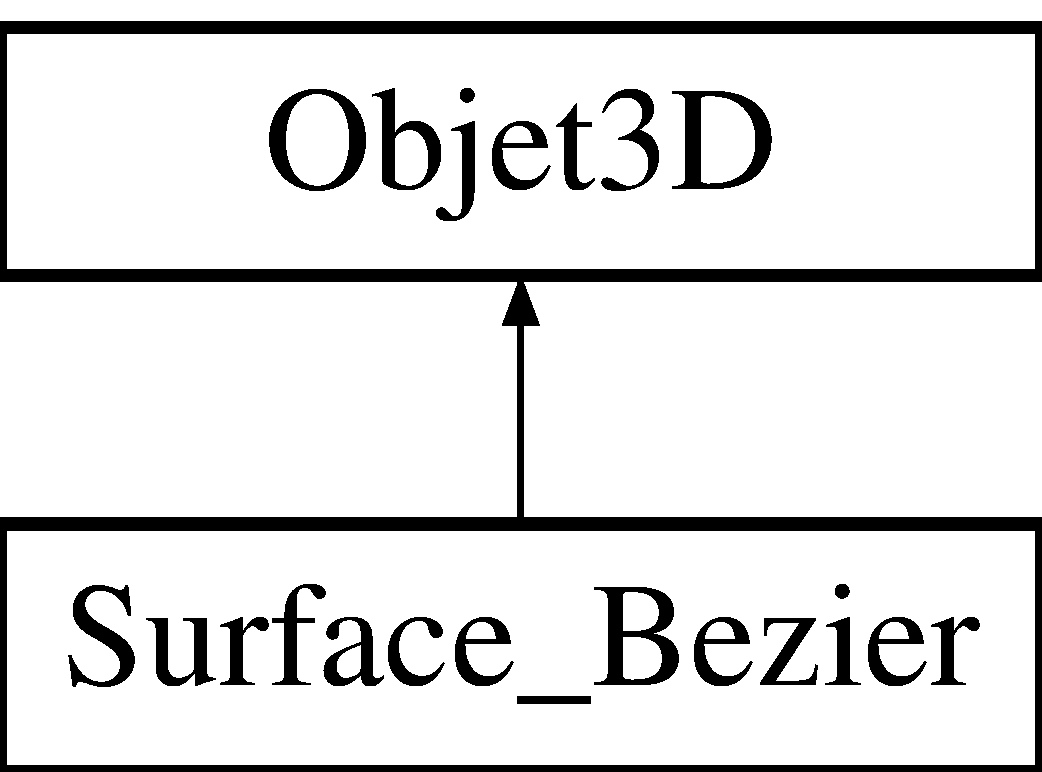
\includegraphics[height=2.000000cm]{classSurface__Bezier}
\end{center}
\end{figure}
\subsection*{Public Member Functions}
\begin{DoxyCompactItemize}
\item 
\hyperlink{classSurface__Bezier_a63f23108ea58f101ede4190e2391b100}{Surface\-\_\-\-Bezier} (std\-::vector$<$ std\-::vector$<$ \hyperlink{classPointGL}{Point\-G\-L} $\ast$ $>$ $>$ lespoints, int nbli, int nbco, float largeur, float hauteur, float longueur)
\begin{DoxyCompactList}\small\item\em Constructeur de la surface de type Bézier. \end{DoxyCompactList}\item 
\hyperlink{classSurface__Bezier_ad0f538994694a94e963e5531dee52ca1}{Surface\-\_\-\-Bezier} (const \hyperlink{classSurface__Bezier}{Surface\-\_\-\-Bezier} \&orig)
\begin{DoxyCompactList}\small\item\em Constructeur en copie. \end{DoxyCompactList}\item 
\hypertarget{classSurface__Bezier_a23912034f978aa1ca017d3804f649bf8}{virtual \hyperlink{classSurface__Bezier_a23912034f978aa1ca017d3804f649bf8}{$\sim$\-Surface\-\_\-\-Bezier} ()}\label{classSurface__Bezier_a23912034f978aa1ca017d3804f649bf8}

\begin{DoxyCompactList}\small\item\em Destructeur de la classe qui détruit les pointeurs. \end{DoxyCompactList}\item 
\hypertarget{classSurface__Bezier_a58a6e683e23d67861cb83cebd81fb93c}{void \hyperlink{classSurface__Bezier_a58a6e683e23d67861cb83cebd81fb93c}{Affichage} ()}\label{classSurface__Bezier_a58a6e683e23d67861cb83cebd81fb93c}

\begin{DoxyCompactList}\small\item\em Fonction permattant l'affichage des points de la surface. \end{DoxyCompactList}\end{DoxyCompactItemize}
\subsection*{Additional Inherited Members}


\subsection{Detailed Description}
\begin{DoxyAuthor}{Author}
P\-O\-N\-C\-I\-A\-N\-O Jean-\/\-Jacques et P\-R\-U\-D\-H\-O\-M\-M\-E Claire 
\end{DoxyAuthor}
\begin{DoxyDate}{Date}
13/03/2014
\end{DoxyDate}
Cette oeuvre, création, code, site ou texte est sous licence Creative Commons Attribution -\/ Pas d’\-Utilisation Commerciale -\/ Partage dans les Mêmes Conditions 4.\-0 International. Pour accéder à une copie de cette licence, merci de vous rendre à l'adresse suivante \href{http://creativecommons.org/licenses/by-nc-sa/4.0/deed.fr}{\tt http\-://creativecommons.\-org/licenses/by-\/nc-\/sa/4.\-0/deed.\-fr} ou envoyez un courrier à Creative Commons, 444 Castro Street, Suite 900, Mountain View, California, 94041, U\-S\-A. Copyright 2014

Contact\-: \href{mailto:ponciano.jeanjacques@gmail.com}{\tt ponciano.\-jeanjacques@gmail.\-com} 

\subsection{Constructor \& Destructor Documentation}
\hypertarget{classSurface__Bezier_a63f23108ea58f101ede4190e2391b100}{\index{Surface\-\_\-\-Bezier@{Surface\-\_\-\-Bezier}!Surface\-\_\-\-Bezier@{Surface\-\_\-\-Bezier}}
\index{Surface\-\_\-\-Bezier@{Surface\-\_\-\-Bezier}!Surface_Bezier@{Surface\-\_\-\-Bezier}}
\subsubsection[{Surface\-\_\-\-Bezier}]{\setlength{\rightskip}{0pt plus 5cm}Surface\-\_\-\-Bezier\-::\-Surface\-\_\-\-Bezier (
\begin{DoxyParamCaption}
\item[{std\-::vector$<$ std\-::vector$<$ {\bf Point\-G\-L} $\ast$ $>$ $>$}]{lespoints, }
\item[{int}]{nbli, }
\item[{int}]{nbco, }
\item[{float}]{largeur, }
\item[{float}]{hauteur, }
\item[{float}]{longueur}
\end{DoxyParamCaption}
)}}\label{classSurface__Bezier_a63f23108ea58f101ede4190e2391b100}


Constructeur de la surface de type Bézier. 


\begin{DoxyParams}{Parameters}
{\em lespoints} & vecteur à 2 dimensions représentant la matrice des points de controle de la surface \\
\hline
{\em nbli} & nombre de lignes de la matrice \\
\hline
{\em nbco} & nombre de colonnes de la matrice \\
\hline
\end{DoxyParams}
\hypertarget{classSurface__Bezier_ad0f538994694a94e963e5531dee52ca1}{\index{Surface\-\_\-\-Bezier@{Surface\-\_\-\-Bezier}!Surface\-\_\-\-Bezier@{Surface\-\_\-\-Bezier}}
\index{Surface\-\_\-\-Bezier@{Surface\-\_\-\-Bezier}!Surface_Bezier@{Surface\-\_\-\-Bezier}}
\subsubsection[{Surface\-\_\-\-Bezier}]{\setlength{\rightskip}{0pt plus 5cm}Surface\-\_\-\-Bezier\-::\-Surface\-\_\-\-Bezier (
\begin{DoxyParamCaption}
\item[{const {\bf Surface\-\_\-\-Bezier} \&}]{orig}
\end{DoxyParamCaption}
)}}\label{classSurface__Bezier_ad0f538994694a94e963e5531dee52ca1}


Constructeur en copie. 


\begin{DoxyParams}{Parameters}
{\em orig} & \\
\hline
\end{DoxyParams}


The documentation for this class was generated from the following files\-:\begin{DoxyCompactItemize}
\item 
modules/open\-G\-L/tools\-\_\-models/\-Surfaces/Surface\-\_\-\-Bezier.\-h\item 
modules/open\-G\-L/tools\-\_\-models/\-Surfaces/Surface\-\_\-\-Bezier.\-cpp\end{DoxyCompactItemize}

\hypertarget{classTexel}{\section{Texel Class Reference}
\label{classTexel}\index{Texel@{Texel}}
}


{\ttfamily \#include $<$Texel.\-h$>$}

\subsection*{Public Member Functions}
\begin{DoxyCompactItemize}
\item 
\hyperlink{classTexel_a8a37c2a61843dd89f0bdde6a8bd37b2c}{Texel} (float x, float y)
\item 
\hypertarget{classTexel_af7f7003572f03860ed85a04abe40e121}{{\bfseries Texel} (const \hyperlink{classTexel}{Texel} \&orig)}\label{classTexel_af7f7003572f03860ed85a04abe40e121}

\item 
float \hyperlink{classTexel_acca976a45b9f06abb496ec35372c6bb8}{get\-X} () const 
\item 
float \hyperlink{classTexel_a9f1c987201a79e0b3ba70e0d0805b7fd}{get\-Y} () const 
\end{DoxyCompactItemize}


\subsection{Detailed Description}
\begin{DoxyAuthor}{Author}
P\-O\-N\-C\-I\-A\-N\-O Jean-\/\-Jacques et P\-R\-U\-D\-H\-O\-M\-M\-E Claire 
\end{DoxyAuthor}
\begin{DoxyDate}{Date}
13/03/2014
\end{DoxyDate}
Cette oeuvre, création, code, site ou texte est sous licence Creative Commons Attribution -\/ Pas d’\-Utilisation Commerciale -\/ Partage dans les Mêmes Conditions 4.\-0 International. Pour accéder à une copie de cette licence, merci de vous rendre à l'adresse suivante \href{http://creativecommons.org/licenses/by-nc-sa/4.0/deed.fr}{\tt http\-://creativecommons.\-org/licenses/by-\/nc-\/sa/4.\-0/deed.\-fr} ou envoyez un courrier à Creative Commons, 444 Castro Street, Suite 900, Mountain View, California, 94041, U\-S\-A. Copyright 2014

Contact\-: \href{mailto:ponciano.jeanjacques@gmail.com}{\tt ponciano.\-jeanjacques@gmail.\-com} 

\subsection{Constructor \& Destructor Documentation}
\hypertarget{classTexel_a8a37c2a61843dd89f0bdde6a8bd37b2c}{\index{Texel@{Texel}!Texel@{Texel}}
\index{Texel@{Texel}!Texel@{Texel}}
\subsubsection[{Texel}]{\setlength{\rightskip}{0pt plus 5cm}Texel\-::\-Texel (
\begin{DoxyParamCaption}
\item[{float}]{x, }
\item[{float}]{y}
\end{DoxyParamCaption}
)}}\label{classTexel_a8a37c2a61843dd89f0bdde6a8bd37b2c}
Construction du point 
\begin{DoxyParams}{Parameters}
{\em x} & abscisse sur l'image \\
\hline
{\em y} & ordonnée dans l'image \\
\hline
\end{DoxyParams}


\subsection{Member Function Documentation}
\hypertarget{classTexel_acca976a45b9f06abb496ec35372c6bb8}{\index{Texel@{Texel}!get\-X@{get\-X}}
\index{get\-X@{get\-X}!Texel@{Texel}}
\subsubsection[{get\-X}]{\setlength{\rightskip}{0pt plus 5cm}float Texel\-::get\-X (
\begin{DoxyParamCaption}
{}
\end{DoxyParamCaption}
) const}}\label{classTexel_acca976a45b9f06abb496ec35372c6bb8}
Récupération de l'abcisse du point \begin{DoxyReturn}{Returns}
l'abscisse sur l'image 
\end{DoxyReturn}
\hypertarget{classTexel_a9f1c987201a79e0b3ba70e0d0805b7fd}{\index{Texel@{Texel}!get\-Y@{get\-Y}}
\index{get\-Y@{get\-Y}!Texel@{Texel}}
\subsubsection[{get\-Y}]{\setlength{\rightskip}{0pt plus 5cm}float Texel\-::get\-Y (
\begin{DoxyParamCaption}
{}
\end{DoxyParamCaption}
) const}}\label{classTexel_a9f1c987201a79e0b3ba70e0d0805b7fd}
Récupération de l'ordonnée du point \begin{DoxyReturn}{Returns}
l'ordonnée sur l'image 
\end{DoxyReturn}


The documentation for this class was generated from the following files\-:\begin{DoxyCompactItemize}
\item 
modules/open\-G\-L/tools\-\_\-models/Texel.\-h\item 
modules/open\-G\-L/tools\-\_\-models/Texel.\-cpp\end{DoxyCompactItemize}

\hypertarget{classTexture}{\section{Texture Class Reference}
\label{classTexture}\index{Texture@{Texture}}
}


{\ttfamily \#include $<$Texture.\-h$>$}

\subsection*{Public Member Functions}
\begin{DoxyCompactItemize}
\item 
\hypertarget{classTexture_a6536fdc1838f905e0319ca7c88e3e58d}{{\bfseries Texture} (Q\-String adresse, std\-::string nom, G\-Luint id)}\label{classTexture_a6536fdc1838f905e0319ca7c88e3e58d}

\item 
\hypertarget{classTexture_abcac6b67c53983ee9e9a99373fe4c925}{{\bfseries Texture} (const \hyperlink{classTexture}{Texture} \&orig)}\label{classTexture_abcac6b67c53983ee9e9a99373fe4c925}

\item 
void \hyperlink{classTexture_a70b86ee52585f20c73e51cf03bb6f6c0}{charger} () const 
\item 
\hypertarget{classTexture_ac795255cc4811d4d57327bd9fecdaef9}{std\-::string {\bfseries get\-Nnom} () const }\label{classTexture_ac795255cc4811d4d57327bd9fecdaef9}

\item 
\hypertarget{classTexture_aa20db484528f539a9557a3193f2a08fb}{G\-Luint {\bfseries get\-Id} () const }\label{classTexture_aa20db484528f539a9557a3193f2a08fb}

\end{DoxyCompactItemize}


\subsection{Detailed Description}
\begin{DoxyAuthor}{Author}
P\-O\-N\-C\-I\-A\-N\-O Jean-\/\-Jacques et P\-R\-U\-D\-H\-O\-M\-M\-E Claire Copyright 2014 P\-O\-N\-C\-I\-A\-N\-O Jean-\/\-Jacques et P\-R\-U\-D\-H\-O\-M\-M\-E Claire Contact\-: \href{mailto:ponciano.jeanjacques@gmail.com}{\tt ponciano.\-jeanjacques@gmail.\-com} Créé le 13 Mars 2014
\end{DoxyAuthor}
Cette oeuvre, création, code, site ou texte est sous licence Creative Commons Attribution -\/ Pas d’\-Utilisation Commerciale -\/ Partage dans les Mêmes Conditions 4.\-0 International. Pour accéder à une copie de cette licence, merci de vous rendre à l'adresse suivante \href{http://creativecommons.org/licenses/by-nc-sa/4.0/deed.fr}{\tt http\-://creativecommons.\-org/licenses/by-\/nc-\/sa/4.\-0/deed.\-fr} ou envoyez un courrier à Creative Commons, 444 Castro Street, Suite 900, Mountain View, California, 94041, U\-S\-A. Installer la librairie libtiff-\/devel sudo yum install libtiff-\/devel.\-x86\-\_\-64 

\subsection{Member Function Documentation}
\hypertarget{classTexture_a70b86ee52585f20c73e51cf03bb6f6c0}{\index{Texture@{Texture}!charger@{charger}}
\index{charger@{charger}!Texture@{Texture}}
\subsubsection[{charger}]{\setlength{\rightskip}{0pt plus 5cm}void Texture\-::charger (
\begin{DoxyParamCaption}
{}
\end{DoxyParamCaption}
) const}}\label{classTexture_a70b86ee52585f20c73e51cf03bb6f6c0}
Affichage de la texture 
\begin{DoxyCode}
   glEnable(GL\_TEXTURE\_2D);
\hyperlink{classTexture_a70b86ee52585f20c73e51cf03bb6f6c0}{charger}();
glTexParameteri(GL\_TEXTURE\_2D, GL\_TEXTURE\_WRAP\_S, GL\_CLAMP);
glTexParameteri(GL\_TEXTURE\_2D, GL\_TEXTURE\_WRAP\_T, GL\_CLAMP);
glTexParameteri(GL\_TEXTURE\_2D, GL\_TEXTURE\_MAG\_FILTER, GL\_NEAREST);
glTexParameteri(GL\_TEXTURE\_2D, GL\_TEXTURE\_MIN\_FILTER, GL\_NEAREST);
glTexEnvf(GL\_TEXTURE\_ENV, GL\_TEXTURE\_ENV\_MODE, GL\_REPLACE);
glBegin(GL\_POLYGON);
\textcolor{keywordflow}{for} (\textcolor{keywordtype}{int} i = 0; i < 6; i++) \{
    \textcolor{keywordtype}{float} x = cos(i * PI / 3.0);
    \textcolor{keywordtype}{float} y = sin(i * PI / 3.0);

    glTexCoord2f((-x + 1) / 2, (-y + 1) / 2);
    glVertex3f(x * 10, y * 10, 0);

\}
glEnd();
glDisable(GL\_TEXTURE\_2D);
\end{DoxyCode}
 

The documentation for this class was generated from the following files\-:\begin{DoxyCompactItemize}
\item 
modules/open\-G\-L/ground/model/Texture.\-h\item 
modules/open\-G\-L/ground/model/Texture.\-cpp\end{DoxyCompactItemize}

\hypertarget{classToolOpenCV}{\section{Tool\-Open\-C\-V Class Reference}
\label{classToolOpenCV}\index{Tool\-Open\-C\-V@{Tool\-Open\-C\-V}}
}


The \hyperlink{classToolOpenCV}{Tool\-Open\-C\-V} class interface entre open\-C\-V et Qt.  




{\ttfamily \#include $<$toolopencv.\-h$>$}

\subsection*{Static Public Member Functions}
\begin{DoxyCompactItemize}
\item 
\hypertarget{classToolOpenCV_a908d7f1eb5ff4f8d44e8fdb822929dc4}{static Q\-Image {\bfseries Ipl2\-Q\-Image} (const Ipl\-Image $\ast$new\-Image)}\label{classToolOpenCV_a908d7f1eb5ff4f8d44e8fdb822929dc4}

\item 
\hypertarget{classToolOpenCV_ab1717ea9b402411b3ac30f3ed8b80075}{static Ipl\-Image $\ast$ {\bfseries Q\-Image2\-Ipl\-Image} (const Q\-Image \&q\-Image)}\label{classToolOpenCV_ab1717ea9b402411b3ac30f3ed8b80075}

\item 
\hypertarget{classToolOpenCV_a5abd7ac7b7fbf8054bbd732693d2cf7b}{static Q\-Image {\bfseries cv\-Mat\-To\-Q\-Image} (const cv\-::\-Mat \&in\-Mat)}\label{classToolOpenCV_a5abd7ac7b7fbf8054bbd732693d2cf7b}

\item 
\hypertarget{classToolOpenCV_ae0bded3d58ff8e333b40dfe5b527c25b}{static cv\-::\-Mat {\bfseries Q\-Image\-To\-Cv\-Mat} (const Q\-Image in\-Image)}\label{classToolOpenCV_ae0bded3d58ff8e333b40dfe5b527c25b}

\end{DoxyCompactItemize}


\subsection{Detailed Description}
The \hyperlink{classToolOpenCV}{Tool\-Open\-C\-V} class interface entre open\-C\-V et Qt. 

The documentation for this class was generated from the following files\-:\begin{DoxyCompactItemize}
\item 
modules/open\-C\-V/ground/model/toolopencv.\-h\item 
modules/open\-C\-V/ground/model/toolopencv.\-cpp\end{DoxyCompactItemize}

\hypertarget{classToolsPCL}{\section{Tools\-P\-C\-L Class Reference}
\label{classToolsPCL}\index{Tools\-P\-C\-L@{Tools\-P\-C\-L}}
}


The \hyperlink{classToolsPCL}{Tools\-P\-C\-L} class for manage pcl This class is used to loading, reading and processing of point clouds.  




{\ttfamily \#include $<$Tools\-P\-C\-L.\-h$>$}

Inheritance diagram for Tools\-P\-C\-L\-:\begin{figure}[H]
\begin{center}
\leavevmode
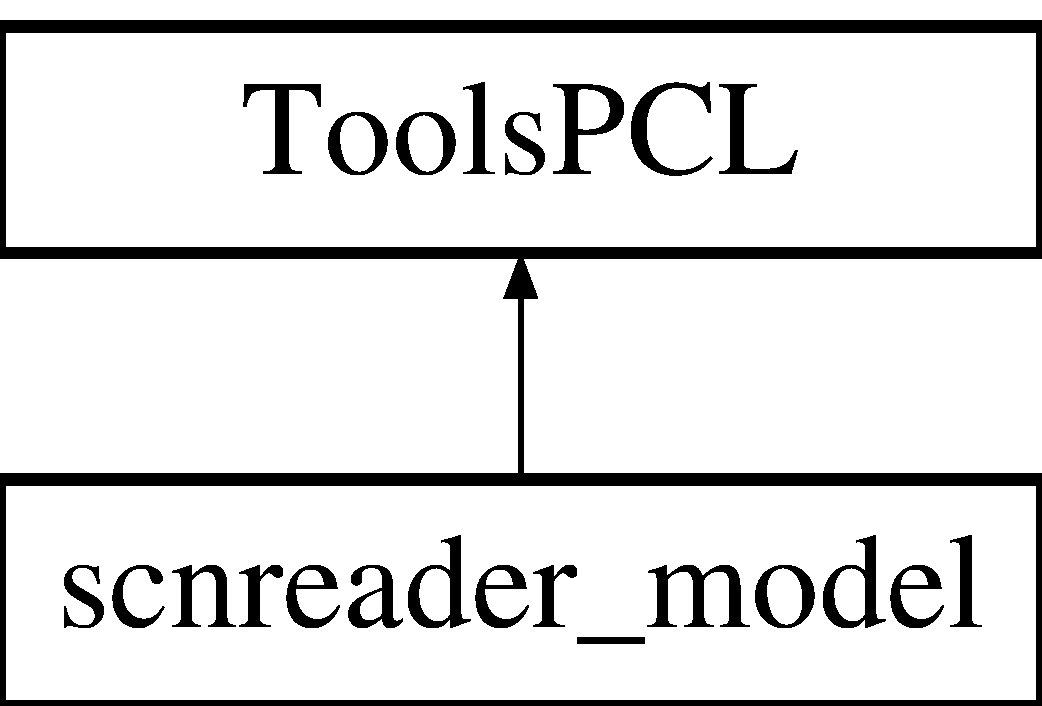
\includegraphics[height=2.000000cm]{classToolsPCL}
\end{center}
\end{figure}
\subsection*{Public Member Functions}
\begin{DoxyCompactItemize}
\item 
\hypertarget{classToolsPCL_a2917407255ebacff1f473337ec45f235}{{\bfseries Tools\-P\-C\-L} (pcl\-::\-Point\-Cloud$<$ pcl\-::\-Point\-X\-Y\-Z $>$\-::Ptr cloud)}\label{classToolsPCL_a2917407255ebacff1f473337ec45f235}

\item 
void \hyperlink{classToolsPCL_ad99c261b21f228056cadade75f04a533}{extraction\-Cloud} (int i)
\begin{DoxyCompactList}\small\item\em extraction\-Cloud create new clouds representing different parts of the cloud located at the ith position in the clouds vector \end{DoxyCompactList}\item 
void \hyperlink{classToolsPCL_a4461f092363e7c30da969950aa6df1a7}{planar\-Segmentation} (int i)
\begin{DoxyCompactList}\small\item\em planar\-Segmentation create a new cloud representing the most larger plan of the cloud located at the ith position in the clouds vector \end{DoxyCompactList}\item 
void \hyperlink{classToolsPCL_a3e2207bc60d537209ef2540b8e23a2ef}{add\-Cloud} (std\-::string pathname)
\begin{DoxyCompactList}\small\item\em add\-Cloud load a cloud from a \char`\"{}pcd\char`\"{} format file and add it in clouds \end{DoxyCompactList}\item 
void \hyperlink{classToolsPCL_a21cf7571eb47821481550218fe292c1b}{add\-Cloud\-From\-T\-X\-T} (std\-::string pathname)
\begin{DoxyCompactList}\small\item\em add\-Cloud load a cloud from a \char`\"{}txt\char`\"{} format file and add it in clouds \end{DoxyCompactList}\item 
void \hyperlink{classToolsPCL_ac81260d8b719c58f84eaf8674691ad12}{save\-Clouds\-From\-T\-X\-T} (std\-::string pathname)
\begin{DoxyCompactList}\small\item\em save\-Clouds\-From\-T\-X\-T save all clouds in \char`\"{}txt\char`\"{} format file \end{DoxyCompactList}\item 
void \hyperlink{classToolsPCL_a181bbd4a2e39bb12dd66b74dbc58425d}{save\-Clouds} (std\-::string pathname)
\begin{DoxyCompactList}\small\item\em save\-Clouds save all clouds in \char`\"{}pcd\char`\"{} format file \end{DoxyCompactList}\item 
Q\-Vector$<$ pcl\-::\-Point\-Cloud\\*
$<$ pcl\-::\-Point\-X\-Y\-Z $>$\-::Ptr $>$ \hyperlink{classToolsPCL_a1eb7da1d719387cb33f75827367ef9f4}{get\-Clouds} ()
\begin{DoxyCompactList}\small\item\em get\-Clouds getter of clouds \end{DoxyCompactList}\item 
pcl\-::\-Point\-Cloud$<$ pcl\-::\-Point\-X\-Y\-Z $>$\\*
\-::Ptr \hyperlink{classToolsPCL_a15e8d38bafcdcf59bbdeb0d8de5fc7d1}{get\-Clouds} (int i)
\begin{DoxyCompactList}\small\item\em get\-Clouds get the cloud has the index i \end{DoxyCompactList}\item 
\hypertarget{classToolsPCL_a4f0f28905620a7ee5f4b0e90980b0334}{void \hyperlink{classToolsPCL_a4f0f28905620a7ee5f4b0e90980b0334}{clear} ()}\label{classToolsPCL_a4f0f28905620a7ee5f4b0e90980b0334}

\begin{DoxyCompactList}\small\item\em clear remove all clouds \end{DoxyCompactList}\item 
\hypertarget{classToolsPCL_a90c5602b7c710f8712fe777e36fe90a8}{float {\bfseries get\-Max\-X} () const }\label{classToolsPCL_a90c5602b7c710f8712fe777e36fe90a8}

\item 
\hypertarget{classToolsPCL_a9f3bf7d917292cc3fca90e98efe57095}{void {\bfseries set\-Max\-X} (float value)}\label{classToolsPCL_a9f3bf7d917292cc3fca90e98efe57095}

\item 
\hypertarget{classToolsPCL_ae29f540eb43bf81e27a449be015b708b}{float {\bfseries get\-Max\-Y} () const }\label{classToolsPCL_ae29f540eb43bf81e27a449be015b708b}

\item 
\hypertarget{classToolsPCL_a4d1993759b3829340585b55d60f4acaf}{void {\bfseries set\-Max\-Y} (float value)}\label{classToolsPCL_a4d1993759b3829340585b55d60f4acaf}

\item 
\hypertarget{classToolsPCL_ac03e32ac82d4ba54d6adeeec55db39f1}{float {\bfseries get\-Max\-Z} () const }\label{classToolsPCL_ac03e32ac82d4ba54d6adeeec55db39f1}

\item 
\hypertarget{classToolsPCL_a1a55b6282fb5e4d6e92282a554422cd5}{void {\bfseries set\-Max\-Z} (float value)}\label{classToolsPCL_a1a55b6282fb5e4d6e92282a554422cd5}

\end{DoxyCompactItemize}
\subsection*{Static Public Member Functions}
\begin{DoxyCompactItemize}
\item 
static pcl\-::\-Point\-Cloud\\*
$<$ pcl\-::\-Point\-X\-Y\-Z\-R\-G\-B $>$\-::Ptr \hyperlink{classToolsPCL_ad7cc79166abda2af6583a6e6033ac003}{get\-Cloud\-Gray} (std\-::string pathname)
\begin{DoxyCompactList}\small\item\em get\-Cloud\-Gray load a gray cloud from file which format is\-: X Y Z grayscale \end{DoxyCompactList}\item 
static pcl\-::\-Point\-Cloud\\*
$<$ pcl\-::\-Point\-X\-Y\-Z $>$\-::Ptr \hyperlink{classToolsPCL_a99f419d563640af3422e5b964d7f9220}{load\-Cloud\-From\-T\-X\-T} (std\-::string pathname)
\begin{DoxyCompactList}\small\item\em load\-Cloud\-From\-T\-X\-T load a cloud from a \char`\"{}txt\char`\"{} format file \end{DoxyCompactList}\item 
static void \hyperlink{classToolsPCL_a247180362526813879137c9dda16d1dc}{save\-Cloud} (pcl\-::\-Point\-Cloud$<$ pcl\-::\-Point\-X\-Y\-Z $>$\-::Ptr cloud, std\-::string new\-Name)
\begin{DoxyCompactList}\small\item\em save\-Cloud save all clouds in \char`\"{}pcd\char`\"{} format file \end{DoxyCompactList}\item 
static void \hyperlink{classToolsPCL_a86b4d1d3f38ebfa68eba60c67f8ec0f6}{save\-Cloud\-From\-T\-X\-T} (pcl\-::\-Point\-Cloud$<$ pcl\-::\-Point\-X\-Y\-Z $>$\-::Ptr cloud, std\-::string pathname)
\begin{DoxyCompactList}\small\item\em save\-Cloud\-From\-T\-X\-T save all clouds in \char`\"{}txt\char`\"{} format file \end{DoxyCompactList}\item 
static pcl\-::\-Point\-Cloud\\*
$<$ pcl\-::\-Point\-X\-Y\-Z\-R\-G\-B $>$\-::Ptr \hyperlink{classToolsPCL_a787a46c37f74aa83e51e7aafdb009b51}{load\-Cloud\-R\-G\-B} (std\-::string pathname)
\begin{DoxyCompactList}\small\item\em load\-Cloud\-R\-G\-B \end{DoxyCompactList}\item 
static pcl\-::\-Point\-Cloud\\*
$<$ pcl\-::\-Point\-X\-Y\-Z $>$\-::Ptr \hyperlink{classToolsPCL_a852f0884ba496b7b2a3a77aabf3923f5}{load\-Cloud} (std\-::string pathname)
\begin{DoxyCompactList}\small\item\em load\-Cloud \end{DoxyCompactList}\item 
static pcl\-::\-Point\-Cloud\\*
$<$ pcl\-::\-Point\-X\-Y\-Z $>$\-::Ptr \hyperlink{classToolsPCL_a302c666bcdd57fd901da32b4581dec5b}{planar\-\_\-segmentation} (pcl\-::\-Point\-Cloud$<$ pcl\-::\-Point\-X\-Y\-Z $>$\-::Ptr cloud)
\begin{DoxyCompactList}\small\item\em planar\-\_\-segmentation create a new cloud representing the most larger plan of the cloud \end{DoxyCompactList}\end{DoxyCompactItemize}
\subsection*{Protected Attributes}
\begin{DoxyCompactItemize}
\item 
\hypertarget{classToolsPCL_a748c8d7a5d782653d3a2afd16d264c21}{float {\bfseries max\-X}}\label{classToolsPCL_a748c8d7a5d782653d3a2afd16d264c21}

\item 
\hypertarget{classToolsPCL_a77aa641be7ca591bfe112d42d3fe84fd}{float {\bfseries max\-Y}}\label{classToolsPCL_a77aa641be7ca591bfe112d42d3fe84fd}

\item 
\hypertarget{classToolsPCL_a5d716f4c7228045bd41d347b262e0e85}{float {\bfseries max\-Z}}\label{classToolsPCL_a5d716f4c7228045bd41d347b262e0e85}

\item 
\hypertarget{classToolsPCL_abeb013b3aadaeedc362e7cf136459e96}{Q\-Vector$<$ pcl\-::\-Point\-Cloud\\*
$<$ pcl\-::\-Point\-X\-Y\-Z $>$\-::Ptr $>$ {\bfseries clouds}}\label{classToolsPCL_abeb013b3aadaeedc362e7cf136459e96}

\end{DoxyCompactItemize}


\subsection{Detailed Description}
The \hyperlink{classToolsPCL}{Tools\-P\-C\-L} class for manage pcl This class is used to loading, reading and processing of point clouds. 

\hypertarget{classToolsPCL_s1}{}\subsection{How to use}\label{classToolsPCL_s1}
\hypertarget{classToolsPCL_subs1}{}\subsubsection{Load cloud}\label{classToolsPCL_subs1}
\hypertarget{classToolsPCL_subs2}{}\paragraph{From pcd file format}\label{classToolsPCL_subs2}
if you want load a cloud from a pcd file format\-: 
\begin{DoxyCode}
std::string pathname=\textcolor{stringliteral}{"myfile.pcd"};
pcl::PointCloud<pcl::PointXYZ>::Ptr cloud=\hyperlink{classToolsPCL_a852f0884ba496b7b2a3a77aabf3923f5}{ToolsPCL::loadCloud}(pathname.c\_str());
\end{DoxyCode}
\hypertarget{classToolsPCL_subs3}{}\paragraph{From T\-X\-T file format}\label{classToolsPCL_subs3}
if you want load a cloud from a T\-X\-T file format\-: 
\begin{DoxyCode}
std::string pathname=\textcolor{stringliteral}{"myfile.TXT"};
pcl::PointCloud<pcl::PointXYZ>::Ptr cloud=\hyperlink{classToolsPCL_a99f419d563640af3422e5b964d7f9220}{ToolsPCL::loadCloudFromTXT}(pathname.
      c\_str());
\end{DoxyCode}
\hypertarget{classToolsPCL_subs4}{}\subsubsection{Save cloud}\label{classToolsPCL_subs4}
\hypertarget{classToolsPCL_subs5}{}\paragraph{To pcd file format}\label{classToolsPCL_subs5}
if you want save a cloud to a pcd file format\-: 
\begin{DoxyCode}
 pcl::PointCloud<pcl::PointXYZ>::Ptr cloud (\textcolor{keyword}{new} pcl::PointCloud<pcl::PointXYZ>);
\hyperlink{classToolsPCL_a247180362526813879137c9dda16d1dc}{ToolsPCL::saveCloud}(cloud,\textcolor{stringliteral}{"myfile.pcd"});
\end{DoxyCode}
\hypertarget{classToolsPCL_subs6}{}\paragraph{To T\-X\-T file format}\label{classToolsPCL_subs6}
if you want save a cloud to a T\-X\-T file format\-: 
\begin{DoxyCode}
 pcl::PointCloud<pcl::PointXYZ>::Ptr cloud (\textcolor{keyword}{new} pcl::PointCloud<pcl::PointXYZ>);
\hyperlink{classToolsPCL_a86b4d1d3f38ebfa68eba60c67f8ec0f6}{ToolsPCL::saveCloudFromTXT}(cloud,\textcolor{stringliteral}{"myfile.TXT"});
\end{DoxyCode}
\hypertarget{classToolsPCL_subs7}{}\subsubsection{Processing}\label{classToolsPCL_subs7}
\hypertarget{classToolsPCL_subs8}{}\paragraph{Planar segmentation}\label{classToolsPCL_subs8}
if you want to execute a planar segmentation\-: 
\begin{DoxyCode}
std::string pathname=\textcolor{stringliteral}{"myfile.pcd"};
pcl::PointCloud<pcl::PointXYZ>::Ptr cloud=\hyperlink{classToolsPCL_a852f0884ba496b7b2a3a77aabf3923f5}{ToolsPCL::loadCloud}(pathname.c\_str());
pcl::PointCloud<pcl::PointXYZ>::Ptr plan=this->\hyperlink{classToolsPCL_a302c666bcdd57fd901da32b4581dec5b}{planar\_segmentation}(cloud);
\end{DoxyCode}
\hypertarget{classToolsPCL_subs9}{}\paragraph{Extraction cluster}\label{classToolsPCL_subs9}
if you want to execute a extraction of different cluser in a cloud\-: 
\begin{DoxyCode}
std::string pathname=\textcolor{stringliteral}{"myfile.pcd"};
pcl::PointCloud<pcl::PointXYZ>::Ptr cloud=\hyperlink{classToolsPCL_a852f0884ba496b7b2a3a77aabf3923f5}{ToolsPCL::loadCloud}(pathname.c\_str());
QStringList cloudsName= this->extractionCloudInList(cloud);
\end{DoxyCode}
 After, you can load all clusters created by using of load\-Cloud with each element in clouds\-Name. Or you can use \hyperlink{classToolsPCL_ad99c261b21f228056cadade75f04a533}{extraction\-Cloud(int i)}. See also exemple\hypertarget{classToolsPCL_subs10}{}\subsubsection{Exemple}\label{classToolsPCL_subs10}
These functions use a array of cloud ( \char`\"{}clouds\char`\"{} in parameters ). You can access this array through \hyperlink{classToolsPCL_a15e8d38bafcdcf59bbdeb0d8de5fc7d1}{get\-Clouds(int i)} or \hyperlink{classToolsPCL_a1eb7da1d719387cb33f75827367ef9f4}{get\-Clouds()} functions. You load a cloud and apply a extraction after a planar segmentation.


\begin{DoxyCode}
  std::string pathname=\textcolor{stringliteral}{"myfile.pcd"};
 \textcolor{comment}{// load cloud}
  pcl::PointCloud<pcl::PointXYZ>::Ptr cloud=\hyperlink{classToolsPCL_a852f0884ba496b7b2a3a77aabf3923f5}{ToolsPCL::loadCloud}(pathname.c\_str());
\textcolor{comment}{//apply planar segmentation}
  pcl::PointCloud<pcl::PointXYZ>::Ptr plan=this->\hyperlink{classToolsPCL_a302c666bcdd57fd901da32b4581dec5b}{planar\_segmentation}(cloud);
\textcolor{comment}{// save in file}
 \hyperlink{classToolsPCL_a86b4d1d3f38ebfa68eba60c67f8ec0f6}{ToolsPCL::saveCloudFromTXT}(plan,\textcolor{stringliteral}{"myfile.TXT"});
\textcolor{comment}{// add this plan in array of cloud}
 \hyperlink{classToolsPCL}{ToolsPCL} tools();
tools.addCloudFromTXT(\textcolor{stringliteral}{"myfile.TXT"});
\textcolor{comment}{// apply extraction}
tools.extractionCloud(0);
\textcolor{comment}{//get the original cloud and all cluster created}
QVector<pcl::PointCloud<pcl::PointXYZ>::Ptr> clustersAndcloud= \hyperlink{classToolsPCL_a1eb7da1d719387cb33f75827367ef9f4}{getClouds}();\textcolor{comment}{// the original cloud
       is at position 0}
\textcolor{comment}{// for fun, save all clouds int txt and pcd files formats}
  \hyperlink{classToolsPCL_ac81260d8b719c58f84eaf8674691ad12}{saveCloudsFromTXT}(\textcolor{stringliteral}{"allc.TXT"});
  \hyperlink{classToolsPCL_a181bbd4a2e39bb12dd66b74dbc58425d}{saveClouds}(\textcolor{stringliteral}{"allc.pcd"});
\end{DoxyCode}
 

\subsection{Member Function Documentation}
\hypertarget{classToolsPCL_a3e2207bc60d537209ef2540b8e23a2ef}{\index{Tools\-P\-C\-L@{Tools\-P\-C\-L}!add\-Cloud@{add\-Cloud}}
\index{add\-Cloud@{add\-Cloud}!ToolsPCL@{Tools\-P\-C\-L}}
\subsubsection[{add\-Cloud}]{\setlength{\rightskip}{0pt plus 5cm}void Tools\-P\-C\-L\-::add\-Cloud (
\begin{DoxyParamCaption}
\item[{std\-::string}]{pathname}
\end{DoxyParamCaption}
)}}\label{classToolsPCL_a3e2207bc60d537209ef2540b8e23a2ef}


add\-Cloud load a cloud from a \char`\"{}pcd\char`\"{} format file and add it in clouds 


\begin{DoxyParams}{Parameters}
{\em pathname} & path of the file for load cloud. \\
\hline
\end{DoxyParams}
\hypertarget{classToolsPCL_a21cf7571eb47821481550218fe292c1b}{\index{Tools\-P\-C\-L@{Tools\-P\-C\-L}!add\-Cloud\-From\-T\-X\-T@{add\-Cloud\-From\-T\-X\-T}}
\index{add\-Cloud\-From\-T\-X\-T@{add\-Cloud\-From\-T\-X\-T}!ToolsPCL@{Tools\-P\-C\-L}}
\subsubsection[{add\-Cloud\-From\-T\-X\-T}]{\setlength{\rightskip}{0pt plus 5cm}void Tools\-P\-C\-L\-::add\-Cloud\-From\-T\-X\-T (
\begin{DoxyParamCaption}
\item[{std\-::string}]{pathname}
\end{DoxyParamCaption}
)}}\label{classToolsPCL_a21cf7571eb47821481550218fe292c1b}


add\-Cloud load a cloud from a \char`\"{}txt\char`\"{} format file and add it in clouds 


\begin{DoxyParams}{Parameters}
{\em pathname} & path of the file for load cloud. \\
\hline
\end{DoxyParams}
\hypertarget{classToolsPCL_ad99c261b21f228056cadade75f04a533}{\index{Tools\-P\-C\-L@{Tools\-P\-C\-L}!extraction\-Cloud@{extraction\-Cloud}}
\index{extraction\-Cloud@{extraction\-Cloud}!ToolsPCL@{Tools\-P\-C\-L}}
\subsubsection[{extraction\-Cloud}]{\setlength{\rightskip}{0pt plus 5cm}void Tools\-P\-C\-L\-::extraction\-Cloud (
\begin{DoxyParamCaption}
\item[{int}]{i}
\end{DoxyParamCaption}
)}}\label{classToolsPCL_ad99c261b21f228056cadade75f04a533}


extraction\-Cloud create new clouds representing different parts of the cloud located at the ith position in the clouds vector 


\begin{DoxyParams}{Parameters}
{\em i} & index of the cloud position in this Qvector clouds \\
\hline
\end{DoxyParams}
\hypertarget{classToolsPCL_ad7cc79166abda2af6583a6e6033ac003}{\index{Tools\-P\-C\-L@{Tools\-P\-C\-L}!get\-Cloud\-Gray@{get\-Cloud\-Gray}}
\index{get\-Cloud\-Gray@{get\-Cloud\-Gray}!ToolsPCL@{Tools\-P\-C\-L}}
\subsubsection[{get\-Cloud\-Gray}]{\setlength{\rightskip}{0pt plus 5cm}pcl\-::\-Point\-Cloud$<$ pcl\-::\-Point\-X\-Y\-Z\-R\-G\-B $>$\-::Ptr Tools\-P\-C\-L\-::get\-Cloud\-Gray (
\begin{DoxyParamCaption}
\item[{std\-::string}]{pathname}
\end{DoxyParamCaption}
)\hspace{0.3cm}{\ttfamily [static]}}}\label{classToolsPCL_ad7cc79166abda2af6583a6e6033ac003}


get\-Cloud\-Gray load a gray cloud from file which format is\-: X Y Z grayscale 


\begin{DoxyParams}{Parameters}
{\em pathname} & path of the file \\
\hline
\end{DoxyParams}
\begin{DoxyReturn}{Returns}
rgb cloud with r=g=b 
\end{DoxyReturn}
\hypertarget{classToolsPCL_a1eb7da1d719387cb33f75827367ef9f4}{\index{Tools\-P\-C\-L@{Tools\-P\-C\-L}!get\-Clouds@{get\-Clouds}}
\index{get\-Clouds@{get\-Clouds}!ToolsPCL@{Tools\-P\-C\-L}}
\subsubsection[{get\-Clouds}]{\setlength{\rightskip}{0pt plus 5cm}Q\-Vector$<$ pcl\-::\-Point\-Cloud$<$ pcl\-::\-Point\-X\-Y\-Z $>$\-::Ptr $>$ Tools\-P\-C\-L\-::get\-Clouds (
\begin{DoxyParamCaption}
{}
\end{DoxyParamCaption}
)}}\label{classToolsPCL_a1eb7da1d719387cb33f75827367ef9f4}


get\-Clouds getter of clouds 

\begin{DoxyReturn}{Returns}
a copy of all clouds 
\end{DoxyReturn}
\hypertarget{classToolsPCL_a15e8d38bafcdcf59bbdeb0d8de5fc7d1}{\index{Tools\-P\-C\-L@{Tools\-P\-C\-L}!get\-Clouds@{get\-Clouds}}
\index{get\-Clouds@{get\-Clouds}!ToolsPCL@{Tools\-P\-C\-L}}
\subsubsection[{get\-Clouds}]{\setlength{\rightskip}{0pt plus 5cm}pcl\-::\-Point\-Cloud$<$ pcl\-::\-Point\-X\-Y\-Z $>$\-::Ptr Tools\-P\-C\-L\-::get\-Clouds (
\begin{DoxyParamCaption}
\item[{int}]{i}
\end{DoxyParamCaption}
)}}\label{classToolsPCL_a15e8d38bafcdcf59bbdeb0d8de5fc7d1}


get\-Clouds get the cloud has the index i 


\begin{DoxyParams}{Parameters}
{\em i} & index of the clouds in class's vector \\
\hline
\end{DoxyParams}
\begin{DoxyReturn}{Returns}
the cloud located at index i of the vector 
\end{DoxyReturn}
\hypertarget{classToolsPCL_a852f0884ba496b7b2a3a77aabf3923f5}{\index{Tools\-P\-C\-L@{Tools\-P\-C\-L}!load\-Cloud@{load\-Cloud}}
\index{load\-Cloud@{load\-Cloud}!ToolsPCL@{Tools\-P\-C\-L}}
\subsubsection[{load\-Cloud}]{\setlength{\rightskip}{0pt plus 5cm}pcl\-::\-Point\-Cloud$<$ pcl\-::\-Point\-X\-Y\-Z $>$\-::Ptr Tools\-P\-C\-L\-::load\-Cloud (
\begin{DoxyParamCaption}
\item[{std\-::string}]{pathname}
\end{DoxyParamCaption}
)\hspace{0.3cm}{\ttfamily [static]}}}\label{classToolsPCL_a852f0884ba496b7b2a3a77aabf3923f5}


load\-Cloud 


\begin{DoxyParams}{Parameters}
{\em pathname} & the path of the load file \\
\hline
\end{DoxyParams}
\begin{DoxyReturn}{Returns}
the cloud save loaded 
\end{DoxyReturn}
\hypertarget{classToolsPCL_a99f419d563640af3422e5b964d7f9220}{\index{Tools\-P\-C\-L@{Tools\-P\-C\-L}!load\-Cloud\-From\-T\-X\-T@{load\-Cloud\-From\-T\-X\-T}}
\index{load\-Cloud\-From\-T\-X\-T@{load\-Cloud\-From\-T\-X\-T}!ToolsPCL@{Tools\-P\-C\-L}}
\subsubsection[{load\-Cloud\-From\-T\-X\-T}]{\setlength{\rightskip}{0pt plus 5cm}pcl\-::\-Point\-Cloud$<$ pcl\-::\-Point\-X\-Y\-Z $>$\-::Ptr Tools\-P\-C\-L\-::load\-Cloud\-From\-T\-X\-T (
\begin{DoxyParamCaption}
\item[{std\-::string}]{pathname}
\end{DoxyParamCaption}
)\hspace{0.3cm}{\ttfamily [static]}}}\label{classToolsPCL_a99f419d563640af3422e5b964d7f9220}


load\-Cloud\-From\-T\-X\-T load a cloud from a \char`\"{}txt\char`\"{} format file 


\begin{DoxyParams}{Parameters}
{\em pathname} & path of the file for load cloud. \\
\hline
\end{DoxyParams}
\begin{DoxyReturn}{Returns}
cloud 
\end{DoxyReturn}
\hypertarget{classToolsPCL_a787a46c37f74aa83e51e7aafdb009b51}{\index{Tools\-P\-C\-L@{Tools\-P\-C\-L}!load\-Cloud\-R\-G\-B@{load\-Cloud\-R\-G\-B}}
\index{load\-Cloud\-R\-G\-B@{load\-Cloud\-R\-G\-B}!ToolsPCL@{Tools\-P\-C\-L}}
\subsubsection[{load\-Cloud\-R\-G\-B}]{\setlength{\rightskip}{0pt plus 5cm}pcl\-::\-Point\-Cloud$<$ pcl\-::\-Point\-X\-Y\-Z\-R\-G\-B $>$\-::Ptr Tools\-P\-C\-L\-::load\-Cloud\-R\-G\-B (
\begin{DoxyParamCaption}
\item[{std\-::string}]{pathname}
\end{DoxyParamCaption}
)\hspace{0.3cm}{\ttfamily [static]}}}\label{classToolsPCL_a787a46c37f74aa83e51e7aafdb009b51}


load\-Cloud\-R\-G\-B 


\begin{DoxyParams}{Parameters}
{\em pathname} & the path of the loqd file \\
\hline
\end{DoxyParams}
\begin{DoxyReturn}{Returns}
the cloud loaded 
\end{DoxyReturn}
\hypertarget{classToolsPCL_a302c666bcdd57fd901da32b4581dec5b}{\index{Tools\-P\-C\-L@{Tools\-P\-C\-L}!planar\-\_\-segmentation@{planar\-\_\-segmentation}}
\index{planar\-\_\-segmentation@{planar\-\_\-segmentation}!ToolsPCL@{Tools\-P\-C\-L}}
\subsubsection[{planar\-\_\-segmentation}]{\setlength{\rightskip}{0pt plus 5cm}pcl\-::\-Point\-Cloud$<$ pcl\-::\-Point\-X\-Y\-Z $>$\-::Ptr Tools\-P\-C\-L\-::planar\-\_\-segmentation (
\begin{DoxyParamCaption}
\item[{pcl\-::\-Point\-Cloud$<$ pcl\-::\-Point\-X\-Y\-Z $>$\-::Ptr}]{cloud}
\end{DoxyParamCaption}
)\hspace{0.3cm}{\ttfamily [static]}}}\label{classToolsPCL_a302c666bcdd57fd901da32b4581dec5b}


planar\-\_\-segmentation create a new cloud representing the most larger plan of the cloud 


\begin{DoxyParams}{Parameters}
{\em cloud} & input cloud \\
\hline
\end{DoxyParams}
\begin{DoxyReturn}{Returns}
A cloud representing the most larger plan of the input cloud in cloud 
\end{DoxyReturn}
\hypertarget{classToolsPCL_a4461f092363e7c30da969950aa6df1a7}{\index{Tools\-P\-C\-L@{Tools\-P\-C\-L}!planar\-Segmentation@{planar\-Segmentation}}
\index{planar\-Segmentation@{planar\-Segmentation}!ToolsPCL@{Tools\-P\-C\-L}}
\subsubsection[{planar\-Segmentation}]{\setlength{\rightskip}{0pt plus 5cm}void Tools\-P\-C\-L\-::planar\-Segmentation (
\begin{DoxyParamCaption}
\item[{int}]{i}
\end{DoxyParamCaption}
)}}\label{classToolsPCL_a4461f092363e7c30da969950aa6df1a7}


planar\-Segmentation create a new cloud representing the most larger plan of the cloud located at the ith position in the clouds vector 


\begin{DoxyParams}{Parameters}
{\em i} & index of the cloud position in this Qvector clouds \\
\hline
\end{DoxyParams}
\hypertarget{classToolsPCL_a247180362526813879137c9dda16d1dc}{\index{Tools\-P\-C\-L@{Tools\-P\-C\-L}!save\-Cloud@{save\-Cloud}}
\index{save\-Cloud@{save\-Cloud}!ToolsPCL@{Tools\-P\-C\-L}}
\subsubsection[{save\-Cloud}]{\setlength{\rightskip}{0pt plus 5cm}void Tools\-P\-C\-L\-::save\-Cloud (
\begin{DoxyParamCaption}
\item[{pcl\-::\-Point\-Cloud$<$ pcl\-::\-Point\-X\-Y\-Z $>$\-::Ptr}]{cloud, }
\item[{std\-::string}]{new\-Name}
\end{DoxyParamCaption}
)\hspace{0.3cm}{\ttfamily [static]}}}\label{classToolsPCL_a247180362526813879137c9dda16d1dc}


save\-Cloud save all clouds in \char`\"{}pcd\char`\"{} format file 


\begin{DoxyParams}{Parameters}
{\em cloud} & the cloud save \\
\hline
{\em new\-Name} & the path of the backup file \\
\hline
\end{DoxyParams}
\hypertarget{classToolsPCL_a86b4d1d3f38ebfa68eba60c67f8ec0f6}{\index{Tools\-P\-C\-L@{Tools\-P\-C\-L}!save\-Cloud\-From\-T\-X\-T@{save\-Cloud\-From\-T\-X\-T}}
\index{save\-Cloud\-From\-T\-X\-T@{save\-Cloud\-From\-T\-X\-T}!ToolsPCL@{Tools\-P\-C\-L}}
\subsubsection[{save\-Cloud\-From\-T\-X\-T}]{\setlength{\rightskip}{0pt plus 5cm}void Tools\-P\-C\-L\-::save\-Cloud\-From\-T\-X\-T (
\begin{DoxyParamCaption}
\item[{pcl\-::\-Point\-Cloud$<$ pcl\-::\-Point\-X\-Y\-Z $>$\-::Ptr}]{cloud, }
\item[{std\-::string}]{pathname}
\end{DoxyParamCaption}
)\hspace{0.3cm}{\ttfamily [static]}}}\label{classToolsPCL_a86b4d1d3f38ebfa68eba60c67f8ec0f6}


save\-Cloud\-From\-T\-X\-T save all clouds in \char`\"{}txt\char`\"{} format file 


\begin{DoxyParams}{Parameters}
{\em cloud} & the cloud save \\
\hline
{\em pathname} & the path of the backup file \\
\hline
\end{DoxyParams}
\hypertarget{classToolsPCL_a181bbd4a2e39bb12dd66b74dbc58425d}{\index{Tools\-P\-C\-L@{Tools\-P\-C\-L}!save\-Clouds@{save\-Clouds}}
\index{save\-Clouds@{save\-Clouds}!ToolsPCL@{Tools\-P\-C\-L}}
\subsubsection[{save\-Clouds}]{\setlength{\rightskip}{0pt plus 5cm}void Tools\-P\-C\-L\-::save\-Clouds (
\begin{DoxyParamCaption}
\item[{std\-::string}]{pathname}
\end{DoxyParamCaption}
)}}\label{classToolsPCL_a181bbd4a2e39bb12dd66b74dbc58425d}


save\-Clouds save all clouds in \char`\"{}pcd\char`\"{} format file 


\begin{DoxyParams}{Parameters}
{\em pathname} & the file path \\
\hline
\end{DoxyParams}
\hypertarget{classToolsPCL_ac81260d8b719c58f84eaf8674691ad12}{\index{Tools\-P\-C\-L@{Tools\-P\-C\-L}!save\-Clouds\-From\-T\-X\-T@{save\-Clouds\-From\-T\-X\-T}}
\index{save\-Clouds\-From\-T\-X\-T@{save\-Clouds\-From\-T\-X\-T}!ToolsPCL@{Tools\-P\-C\-L}}
\subsubsection[{save\-Clouds\-From\-T\-X\-T}]{\setlength{\rightskip}{0pt plus 5cm}void Tools\-P\-C\-L\-::save\-Clouds\-From\-T\-X\-T (
\begin{DoxyParamCaption}
\item[{std\-::string}]{pathname}
\end{DoxyParamCaption}
)}}\label{classToolsPCL_ac81260d8b719c58f84eaf8674691ad12}


save\-Clouds\-From\-T\-X\-T save all clouds in \char`\"{}txt\char`\"{} format file 


\begin{DoxyParams}{Parameters}
{\em pathname} & the file path \\
\hline
\end{DoxyParams}


The documentation for this class was generated from the following files\-:\begin{DoxyCompactItemize}
\item 
modules/pcl/ground/\hyperlink{ToolsPCL_8h}{Tools\-P\-C\-L.\-h}\item 
modules/pcl/ground/Tools\-P\-C\-L.\-cpp\end{DoxyCompactItemize}

\hypertarget{classTore}{\section{Tore Class Reference}
\label{classTore}\index{Tore@{Tore}}
}


{\ttfamily \#include $<$Tore.\-h$>$}

Inheritance diagram for Tore\-:\begin{figure}[H]
\begin{center}
\leavevmode
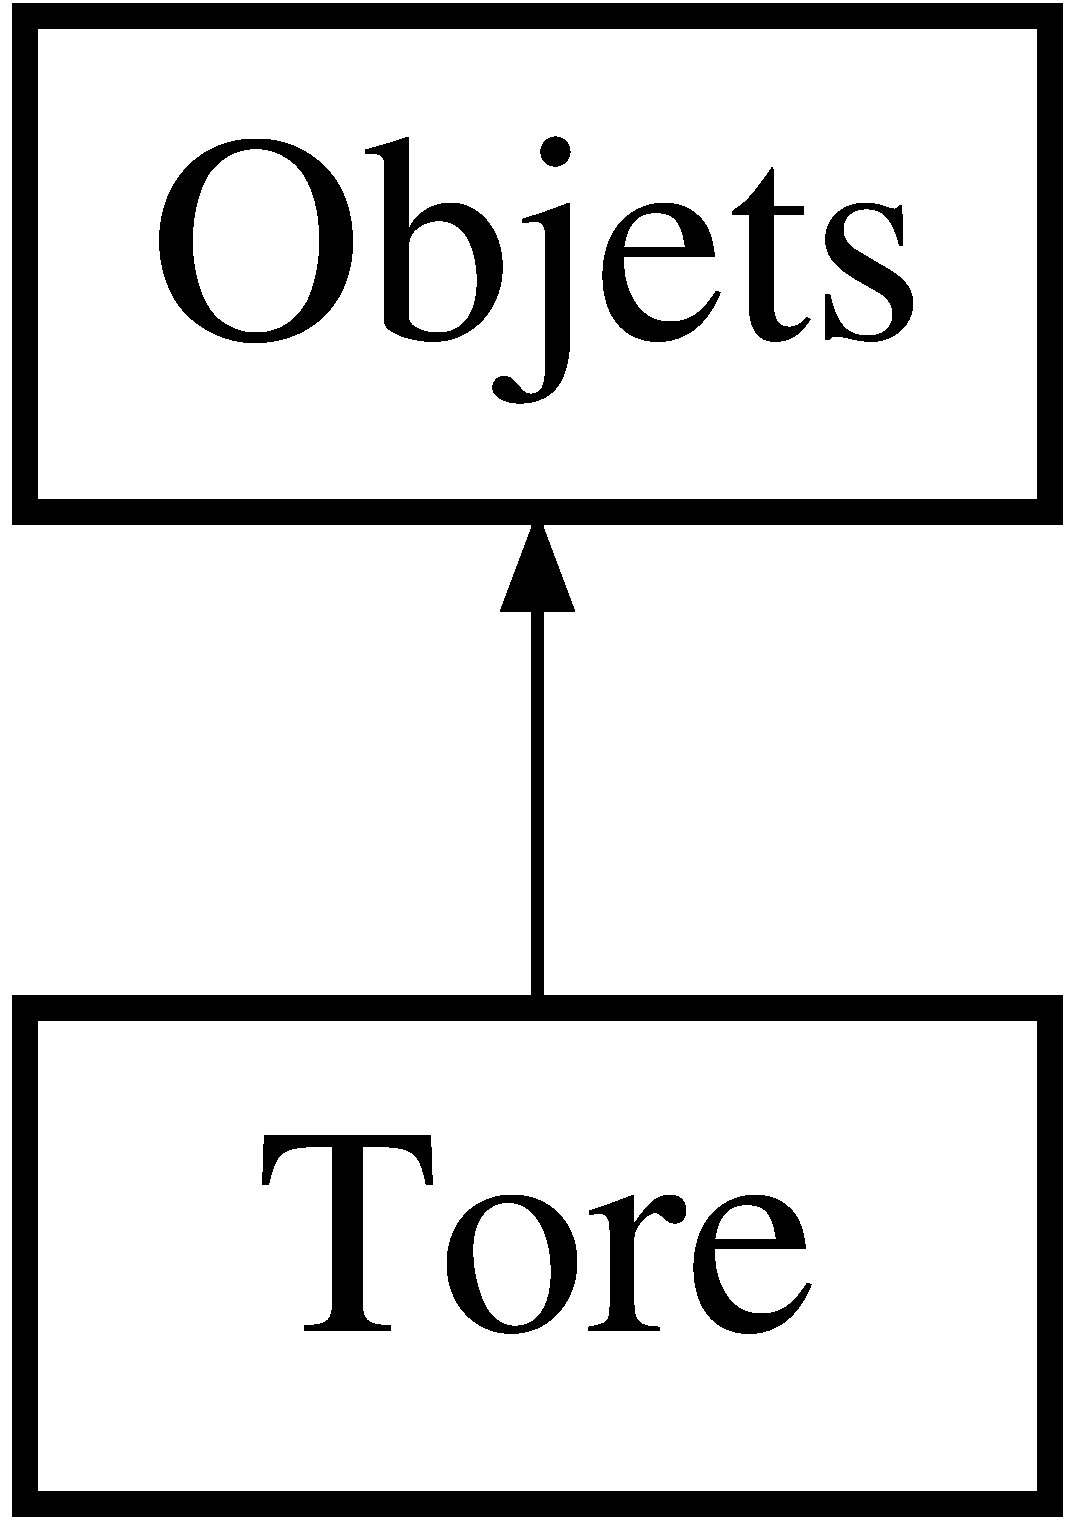
\includegraphics[height=2.000000cm]{classTore}
\end{center}
\end{figure}
\subsection*{Public Member Functions}
\begin{DoxyCompactItemize}
\item 
\hyperlink{classTore_a9462794ae1f45462fc36494948b91e30}{Tore} ()
\begin{DoxyCompactList}\small\item\em Construit un tore avec 100 parallèles et meridient de diamètre 2 et 1. \end{DoxyCompactList}\item 
\hyperlink{classTore_a3f8424c442e311c57da21d9736b36603}{Tore} (float r, float R, int parallele, int meridien)
\item 
\hyperlink{classTore_ad9bb3f3d16fd81888cc343261f89263a}{Tore} (const \hyperlink{classTore}{Tore} \&orig)
\item 
void \hyperlink{classTore_acfda6ef660e1a3f3f8c9e78cdb63a629}{construction} ()
\item 
void \hyperlink{classTore_a9f03eb71804801cd86ba7aefa3a16399}{affiche\-Points} () const 
\item 
void \hyperlink{classTore_a4b082286667409f8dfa9a936d2e6c37b}{affichage} () const 
\item 
void \hyperlink{classTore_a0b432929588d434992e84b8b25fd73eb}{set\-Couleur} (float r, float g, float b)
\item 
void \hyperlink{classTore_af296d4d63dba7cea14e93522e6eb39af}{set\-Couleur} (const \hyperlink{classCouleur}{Couleur} \&c)
\end{DoxyCompactItemize}
\subsection*{Additional Inherited Members}


\subsection{Detailed Description}
\begin{DoxyAuthor}{Author}
P\-O\-N\-C\-I\-A\-N\-O Jean-\/\-Jacques et P\-R\-U\-D\-H\-O\-M\-M\-E Claire 
\end{DoxyAuthor}
\begin{DoxyDate}{Date}
13/03/2014
\end{DoxyDate}
Cette oeuvre, création, code, site ou texte est sous licence Creative Commons Attribution -\/ Pas d’\-Utilisation Commerciale -\/ Partage dans les Mêmes Conditions 4.\-0 International. Pour accéder à une copie de cette licence, merci de vous rendre à l'adresse suivante \href{http://creativecommons.org/licenses/by-nc-sa/4.0/deed.fr}{\tt http\-://creativecommons.\-org/licenses/by-\/nc-\/sa/4.\-0/deed.\-fr} ou envoyez un courrier à Creative Commons, 444 Castro Street, Suite 900, Mountain View, California, 94041, U\-S\-A. Copyright 2014

Contact\-: \href{mailto:ponciano.jeanjacques@gmail.com}{\tt ponciano.\-jeanjacques@gmail.\-com} Création d'un tore facétisé 
\begin{DoxyCode}
\hyperlink{classTore}{Tore} tore(4,3,100,100); 
tore.affichage();
\end{DoxyCode}
 

\subsection{Constructor \& Destructor Documentation}
\hypertarget{classTore_a9462794ae1f45462fc36494948b91e30}{\index{Tore@{Tore}!Tore@{Tore}}
\index{Tore@{Tore}!Tore@{Tore}}
\subsubsection[{Tore}]{\setlength{\rightskip}{0pt plus 5cm}Tore\-::\-Tore (
\begin{DoxyParamCaption}
{}
\end{DoxyParamCaption}
)}}\label{classTore_a9462794ae1f45462fc36494948b91e30}


Construit un tore avec 100 parallèles et meridient de diamètre 2 et 1. 

Constructeur \hypertarget{classTore_a3f8424c442e311c57da21d9736b36603}{\index{Tore@{Tore}!Tore@{Tore}}
\index{Tore@{Tore}!Tore@{Tore}}
\subsubsection[{Tore}]{\setlength{\rightskip}{0pt plus 5cm}Tore\-::\-Tore (
\begin{DoxyParamCaption}
\item[{float}]{r, }
\item[{float}]{R, }
\item[{int}]{parallele, }
\item[{int}]{meridien}
\end{DoxyParamCaption}
)}}\label{classTore_a3f8424c442e311c57da21d9736b36603}
Constructeur 
\begin{DoxyParams}{Parameters}
{\em R} & distance entre le centre du tube et le centre du tore \\
\hline
{\em r} & est le rayon du cercle \\
\hline
{\em parallele} & nomvre de parallèles \\
\hline
{\em meridien} & nombre de méridient 
\begin{DoxyCode}
\hyperlink{classTore}{Tore} tore(4,3,100,100); 
\end{DoxyCode}
 \\
\hline
\end{DoxyParams}
\hypertarget{classTore_ad9bb3f3d16fd81888cc343261f89263a}{\index{Tore@{Tore}!Tore@{Tore}}
\index{Tore@{Tore}!Tore@{Tore}}
\subsubsection[{Tore}]{\setlength{\rightskip}{0pt plus 5cm}Tore\-::\-Tore (
\begin{DoxyParamCaption}
\item[{const {\bf Tore} \&}]{orig}
\end{DoxyParamCaption}
)}}\label{classTore_ad9bb3f3d16fd81888cc343261f89263a}
Constructeur de copie 
\begin{DoxyParams}{Parameters}
{\em orig} & tore à copier \\
\hline
\end{DoxyParams}


\subsection{Member Function Documentation}
\hypertarget{classTore_a4b082286667409f8dfa9a936d2e6c37b}{\index{Tore@{Tore}!affichage@{affichage}}
\index{affichage@{affichage}!Tore@{Tore}}
\subsubsection[{affichage}]{\setlength{\rightskip}{0pt plus 5cm}void Tore\-::affichage (
\begin{DoxyParamCaption}
{}
\end{DoxyParamCaption}
) const}}\label{classTore_a4b082286667409f8dfa9a936d2e6c37b}
Affiche le tore sous forme de facette \hypertarget{classTore_a9f03eb71804801cd86ba7aefa3a16399}{\index{Tore@{Tore}!affiche\-Points@{affiche\-Points}}
\index{affiche\-Points@{affiche\-Points}!Tore@{Tore}}
\subsubsection[{affiche\-Points}]{\setlength{\rightskip}{0pt plus 5cm}void Tore\-::affiche\-Points (
\begin{DoxyParamCaption}
{}
\end{DoxyParamCaption}
) const}}\label{classTore_a9f03eb71804801cd86ba7aefa3a16399}
Affiche chaque point du tore \hypertarget{classTore_acfda6ef660e1a3f3f8c9e78cdb63a629}{\index{Tore@{Tore}!construction@{construction}}
\index{construction@{construction}!Tore@{Tore}}
\subsubsection[{construction}]{\setlength{\rightskip}{0pt plus 5cm}void Tore\-::construction (
\begin{DoxyParamCaption}
{}
\end{DoxyParamCaption}
)\hspace{0.3cm}{\ttfamily [virtual]}}}\label{classTore_acfda6ef660e1a3f3f8c9e78cdb63a629}
Calcule tous les points du tore 

Reimplemented from \hyperlink{classObjets_a2c14a4a3841d82cef1d1ef4e695859f6}{Objets}.

\hypertarget{classTore_a0b432929588d434992e84b8b25fd73eb}{\index{Tore@{Tore}!set\-Couleur@{set\-Couleur}}
\index{set\-Couleur@{set\-Couleur}!Tore@{Tore}}
\subsubsection[{set\-Couleur}]{\setlength{\rightskip}{0pt plus 5cm}void Tore\-::set\-Couleur (
\begin{DoxyParamCaption}
\item[{float}]{r, }
\item[{float}]{g, }
\item[{float}]{b}
\end{DoxyParamCaption}
)}}\label{classTore_a0b432929588d434992e84b8b25fd73eb}
Affecte une couleur aux faces 
\begin{DoxyParams}{Parameters}
{\em r} & canal rouge \\
\hline
{\em g} & canal vert \\
\hline
{\em b} & canal bleu \\
\hline
\end{DoxyParams}
\hypertarget{classTore_af296d4d63dba7cea14e93522e6eb39af}{\index{Tore@{Tore}!set\-Couleur@{set\-Couleur}}
\index{set\-Couleur@{set\-Couleur}!Tore@{Tore}}
\subsubsection[{set\-Couleur}]{\setlength{\rightskip}{0pt plus 5cm}void Tore\-::set\-Couleur (
\begin{DoxyParamCaption}
\item[{const {\bf Couleur} \&}]{c}
\end{DoxyParamCaption}
)}}\label{classTore_af296d4d63dba7cea14e93522e6eb39af}
Affecte une couleur aux faces 
\begin{DoxyParams}{Parameters}
{\em c} & couleur \\
\hline
\end{DoxyParams}


The documentation for this class was generated from the following files\-:\begin{DoxyCompactItemize}
\item 
modules/open\-G\-L/tools\-\_\-models/objets/Tore.\-h\item 
modules/open\-G\-L/tools\-\_\-models/objets/Tore.\-cpp\end{DoxyCompactItemize}

\hypertarget{classView__ground__GL}{\section{View\-\_\-ground\-\_\-\-G\-L Class Reference}
\label{classView__ground__GL}\index{View\-\_\-ground\-\_\-\-G\-L@{View\-\_\-ground\-\_\-\-G\-L}}
}
Inheritance diagram for View\-\_\-ground\-\_\-\-G\-L\-:\begin{figure}[H]
\begin{center}
\leavevmode
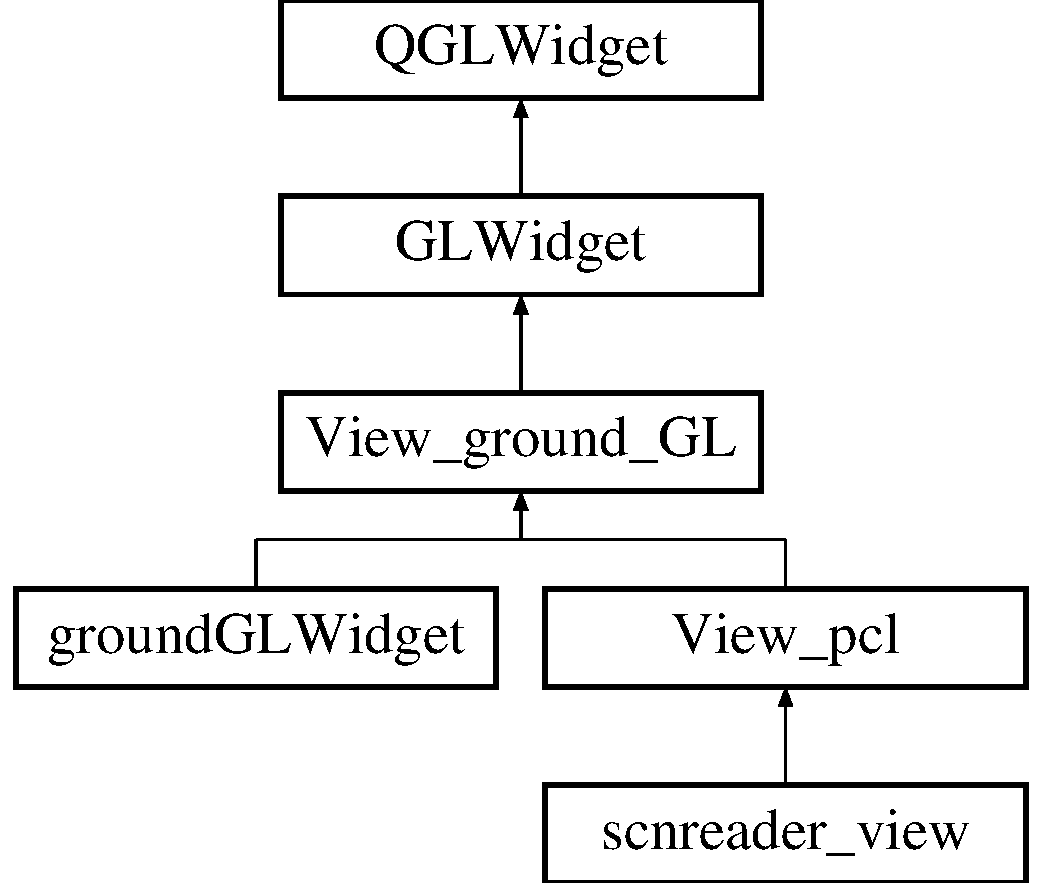
\includegraphics[height=5.000000cm]{classView__ground__GL}
\end{center}
\end{figure}
\subsection*{Public Member Functions}
\begin{DoxyCompactItemize}
\item 
\hypertarget{classView__ground__GL_ad280fec3ac587e32b1aeb42275f4bee1}{{\bfseries View\-\_\-ground\-\_\-\-G\-L} (Q\-Widget $\ast$parent=0)}\label{classView__ground__GL_ad280fec3ac587e32b1aeb42275f4bee1}

\item 
\hypertarget{classView__ground__GL_ae7eb5bc5e8d619708c4cec03e8f7c6d8}{void {\bfseries resize\-G\-L} (int ratio, int height)}\label{classView__ground__GL_ae7eb5bc5e8d619708c4cec03e8f7c6d8}

\item 
\hypertarget{classView__ground__GL_a99b642d0e4edb0c28da8388ea6e5f554}{void {\bfseries initialize\-G\-L} ()}\label{classView__ground__GL_a99b642d0e4edb0c28da8388ea6e5f554}

\item 
\hypertarget{classView__ground__GL_a2f99317cb82dad07eeeef70fe5f922af}{void {\bfseries paint\-G\-L} ()}\label{classView__ground__GL_a2f99317cb82dad07eeeef70fe5f922af}

\item 
\hypertarget{classView__ground__GL_a0345ad5bad48bfd071bc3e75bc462418}{virtual void {\bfseries key\-Press\-Event} (Q\-Key\-Event $\ast$key\-Event)}\label{classView__ground__GL_a0345ad5bad48bfd071bc3e75bc462418}

\item 
\hypertarget{classView__ground__GL_af78b4d515163a34b140d08a8bc100c5b}{virtual void {\bfseries mouse\-Press\-Event} (Q\-Mouse\-Event $\ast$event)}\label{classView__ground__GL_af78b4d515163a34b140d08a8bc100c5b}

\item 
\hypertarget{classView__ground__GL_ac790d474860b0bde374f08cdfb2471f2}{virtual void {\bfseries mouse\-Release\-Event} (Q\-Mouse\-Event $\ast$event)}\label{classView__ground__GL_ac790d474860b0bde374f08cdfb2471f2}

\item 
\hypertarget{classView__ground__GL_a1c78b975b798824d45c7204b25fc24c4}{virtual void {\bfseries mouse\-Move\-Event} (Q\-Mouse\-Event $\ast$event)}\label{classView__ground__GL_a1c78b975b798824d45c7204b25fc24c4}

\end{DoxyCompactItemize}
\subsection*{Additional Inherited Members}


The documentation for this class was generated from the following files\-:\begin{DoxyCompactItemize}
\item 
modules/open\-G\-L/ground/view/view\-\_\-ground\-\_\-\-G\-L.\-h\item 
modules/open\-G\-L/ground/view/view\-\_\-ground\-\_\-\-G\-L.\-cpp\end{DoxyCompactItemize}

\hypertarget{classView__pcl}{\section{View\-\_\-pcl Class Reference}
\label{classView__pcl}\index{View\-\_\-pcl@{View\-\_\-pcl}}
}
Inheritance diagram for View\-\_\-pcl\-:\begin{figure}[H]
\begin{center}
\leavevmode
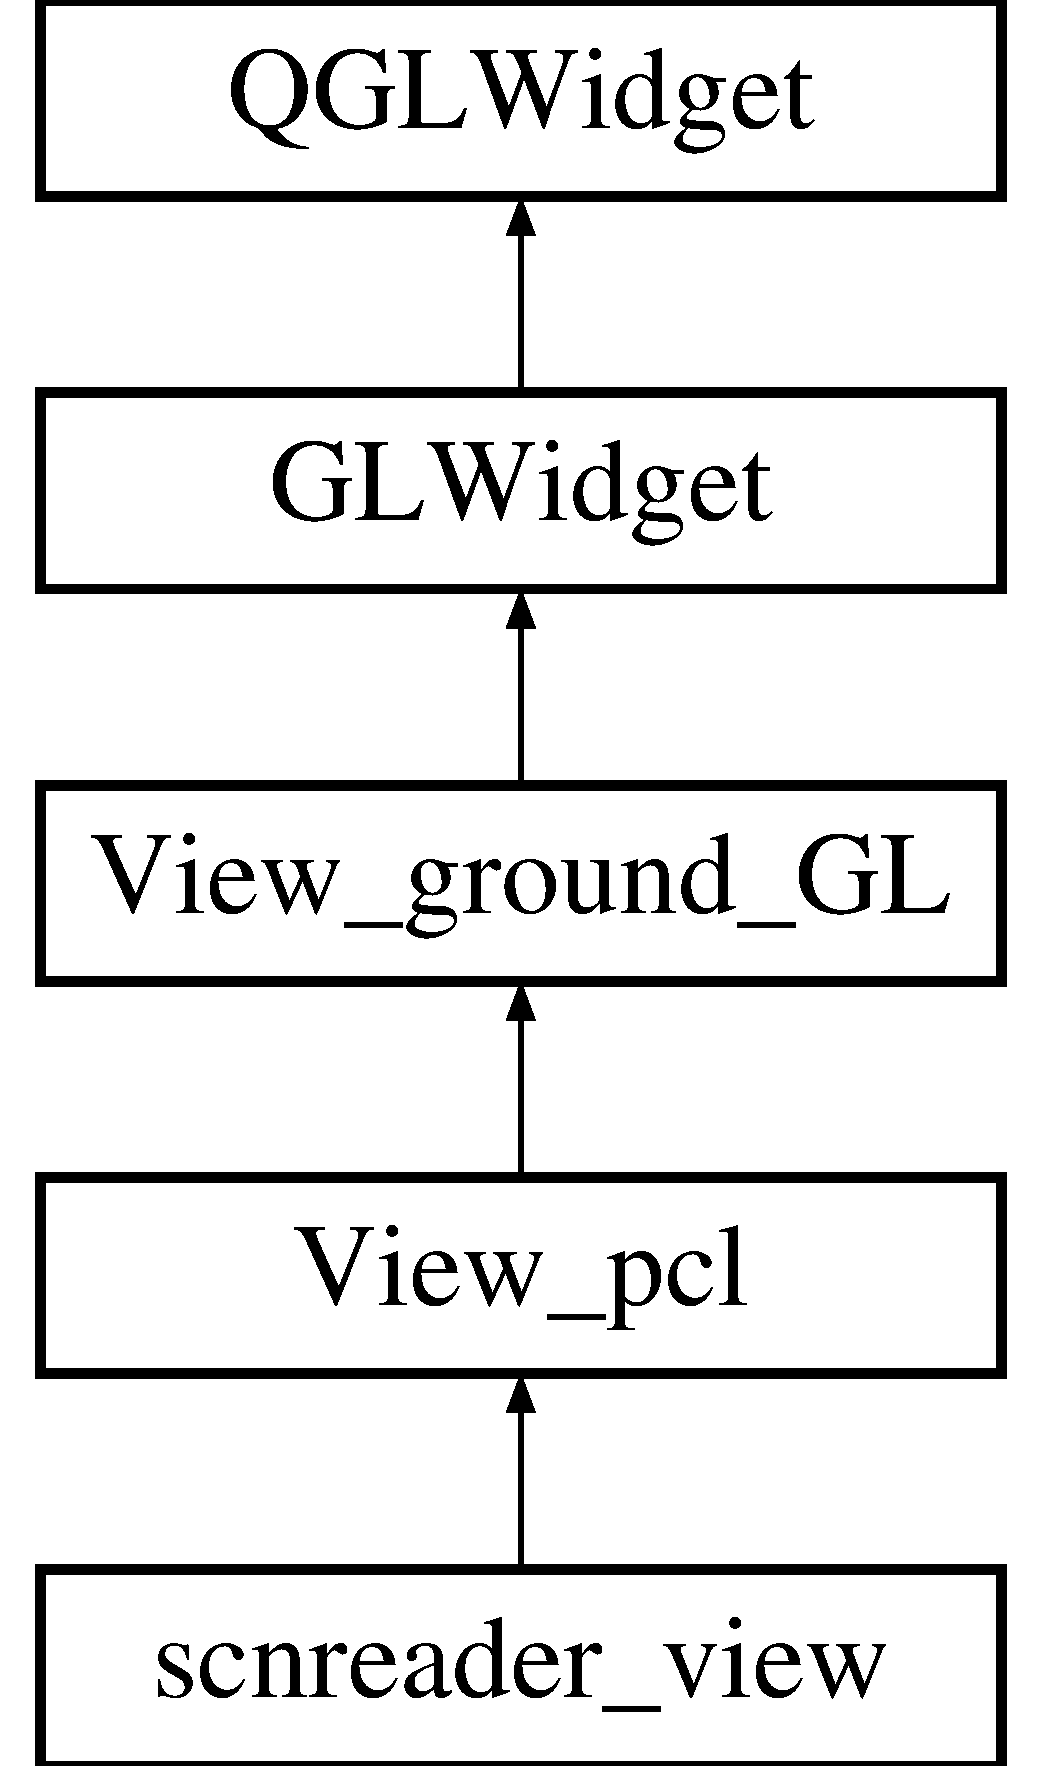
\includegraphics[height=5.000000cm]{classView__pcl}
\end{center}
\end{figure}
\subsection*{Public Member Functions}
\begin{DoxyCompactItemize}
\item 
\hypertarget{classView__pcl_a7b69a39591374ced8ce47dfec309fdeb}{{\bfseries View\-\_\-pcl} (Q\-Widget $\ast$parent=0)}\label{classView__pcl_a7b69a39591374ced8ce47dfec309fdeb}

\item 
\hypertarget{classView__pcl_a51b12206778f93628545cb35c0df1a0e}{void {\bfseries resize\-G\-L} (int ratio, int height)}\label{classView__pcl_a51b12206778f93628545cb35c0df1a0e}

\item 
\hypertarget{classView__pcl_aa1ce55fc6eee5a8701fe1337d9798e6c}{void {\bfseries initialize\-G\-L} ()}\label{classView__pcl_aa1ce55fc6eee5a8701fe1337d9798e6c}

\item 
\hypertarget{classView__pcl_a421a85e2accc0ca3456210a467abe4a3}{void {\bfseries paint\-G\-L} ()}\label{classView__pcl_a421a85e2accc0ca3456210a467abe4a3}

\item 
\hypertarget{classView__pcl_ada831985f6aa0e7387a397790344d5c2}{virtual void {\bfseries key\-Press\-Event} (Q\-Key\-Event $\ast$key\-Event)}\label{classView__pcl_ada831985f6aa0e7387a397790344d5c2}

\item 
\hypertarget{classView__pcl_abb0ce71258b659307a2061f19fbb7492}{virtual void {\bfseries mouse\-Press\-Event} (Q\-Mouse\-Event $\ast$event)}\label{classView__pcl_abb0ce71258b659307a2061f19fbb7492}

\item 
\hypertarget{classView__pcl_ad6d04640841f88e05dc4c7c0e7f836a9}{virtual void {\bfseries mouse\-Release\-Event} (Q\-Mouse\-Event $\ast$event)}\label{classView__pcl_ad6d04640841f88e05dc4c7c0e7f836a9}

\item 
\hypertarget{classView__pcl_ae2a1385eb0fb5cfbe9f9fe5b20c5e72c}{virtual void {\bfseries mouse\-Move\-Event} (Q\-Mouse\-Event $\ast$event)}\label{classView__pcl_ae2a1385eb0fb5cfbe9f9fe5b20c5e72c}

\item 
\hypertarget{classView__pcl_ac5dfc49601a4752d9881b01edd5eb3a3}{void \hyperlink{classView__pcl_ac5dfc49601a4752d9881b01edd5eb3a3}{clear} ()}\label{classView__pcl_ac5dfc49601a4752d9881b01edd5eb3a3}

\begin{DoxyCompactList}\small\item\em clear remove all clouds \end{DoxyCompactList}\item 
void \hyperlink{classView__pcl_abb07264cf45714a7531fa36a968a6a3c}{extraction\-Cloud} (int i)
\begin{DoxyCompactList}\small\item\em extraction\-Cloud create new clouds representing different parts of the cloud located at the ith position in the clouds vector \end{DoxyCompactList}\item 
void \hyperlink{classView__pcl_a6823105f34b5215f1c085b9c5233d216}{planar\-Segmentation} (int i)
\begin{DoxyCompactList}\small\item\em planar\-Segmentation create a new cloud representing the most larger plan of the cloud located at the ith position in the clouds vector \end{DoxyCompactList}\item 
\hypertarget{classView__pcl_a48b72b9d7b7616cfe25d028fe88fb641}{void \hyperlink{classView__pcl_a48b72b9d7b7616cfe25d028fe88fb641}{load\-Cloud} ()}\label{classView__pcl_a48b72b9d7b7616cfe25d028fe88fb641}

\begin{DoxyCompactList}\small\item\em load\-Cloud Opens a window allowing the user to select the file to load and load the cloud from file. The format of the file is \char`\"{}pcd\char`\"{} \end{DoxyCompactList}\item 
\hypertarget{classView__pcl_a684dfd64aca0283a5d286343db04f131}{void \hyperlink{classView__pcl_a684dfd64aca0283a5d286343db04f131}{load\-Cloud\-From\-T\-X\-T} ()}\label{classView__pcl_a684dfd64aca0283a5d286343db04f131}

\begin{DoxyCompactList}\small\item\em load\-Cloud\-From\-T\-X\-T Opens a window allowing the user to select the file to load and load the cloud from file. The format of the file is \char`\"{}text\char`\"{} \end{DoxyCompactList}\item 
\hypertarget{classView__pcl_a8ef1ed1a4c521243d43af150f0ded63b}{void \hyperlink{classView__pcl_a8ef1ed1a4c521243d43af150f0ded63b}{save\-Clouds\-From\-T\-X\-T} ()}\label{classView__pcl_a8ef1ed1a4c521243d43af150f0ded63b}

\begin{DoxyCompactList}\small\item\em save\-Clouds\-From\-T\-X\-T Opens a window allowing the user to select destination to save all clouds in \char`\"{}txt\char`\"{} format file and save it \end{DoxyCompactList}\item 
\hypertarget{classView__pcl_a2f59d02b504d216425642b5c40bf6f76}{void \hyperlink{classView__pcl_a2f59d02b504d216425642b5c40bf6f76}{save\-Clouds} ()}\label{classView__pcl_a2f59d02b504d216425642b5c40bf6f76}

\begin{DoxyCompactList}\small\item\em save\-Clouds Opens a window allowing the user to select destination to save all clouds in \char`\"{}pcd\char`\"{} format file and save it \end{DoxyCompactList}\end{DoxyCompactItemize}
\subsection*{Protected Attributes}
\begin{DoxyCompactItemize}
\item 
\hypertarget{classView__pcl_a6cc80ce45375062a3a8a647ba3e850d9}{\hyperlink{classToolsPCL}{Tools\-P\-C\-L} {\bfseries toolspcl}}\label{classView__pcl_a6cc80ce45375062a3a8a647ba3e850d9}

\item 
\hypertarget{classView__pcl_af68d75a748c82f176d9d6bc99944d7bc}{int {\bfseries size\-Cloud}}\label{classView__pcl_af68d75a748c82f176d9d6bc99944d7bc}

\end{DoxyCompactItemize}
\subsection*{Additional Inherited Members}


\subsection{Member Function Documentation}
\hypertarget{classView__pcl_abb07264cf45714a7531fa36a968a6a3c}{\index{View\-\_\-pcl@{View\-\_\-pcl}!extraction\-Cloud@{extraction\-Cloud}}
\index{extraction\-Cloud@{extraction\-Cloud}!View_pcl@{View\-\_\-pcl}}
\subsubsection[{extraction\-Cloud}]{\setlength{\rightskip}{0pt plus 5cm}void View\-\_\-pcl\-::extraction\-Cloud (
\begin{DoxyParamCaption}
\item[{int}]{i}
\end{DoxyParamCaption}
)}}\label{classView__pcl_abb07264cf45714a7531fa36a968a6a3c}


extraction\-Cloud create new clouds representing different parts of the cloud located at the ith position in the clouds vector 


\begin{DoxyParams}{Parameters}
{\em i} & index of the cloud position in this Qvector clouds \\
\hline
\end{DoxyParams}
\hypertarget{classView__pcl_a6823105f34b5215f1c085b9c5233d216}{\index{View\-\_\-pcl@{View\-\_\-pcl}!planar\-Segmentation@{planar\-Segmentation}}
\index{planar\-Segmentation@{planar\-Segmentation}!View_pcl@{View\-\_\-pcl}}
\subsubsection[{planar\-Segmentation}]{\setlength{\rightskip}{0pt plus 5cm}void View\-\_\-pcl\-::planar\-Segmentation (
\begin{DoxyParamCaption}
\item[{int}]{i}
\end{DoxyParamCaption}
)}}\label{classView__pcl_a6823105f34b5215f1c085b9c5233d216}


planar\-Segmentation create a new cloud representing the most larger plan of the cloud located at the ith position in the clouds vector 


\begin{DoxyParams}{Parameters}
{\em i} & index of the cloud position in this Qvector clouds \\
\hline
\end{DoxyParams}


The documentation for this class was generated from the following files\-:\begin{DoxyCompactItemize}
\item 
modules/pcl/view/view\-\_\-pcl.\-h\item 
modules/pcl/view/view\-\_\-pcl.\-cpp\end{DoxyCompactItemize}

\chapter{File Documentation}
\hypertarget{erreur_8h}{\section{modules/exceptions/erreur.h File Reference}
\label{erreur_8h}\index{modules/exceptions/erreur.\-h@{modules/exceptions/erreur.\-h}}
}


file to the managements of exeptions  


{\ttfamily \#include $<$exception$>$}\\*
{\ttfamily \#include $<$string$>$}\\*
\subsection*{Classes}
\begin{DoxyCompactItemize}
\item 
class \hyperlink{classErreur}{Erreur}
\begin{DoxyCompactList}\small\item\em The \hyperlink{classErreur}{Erreur} class for manage exeptions This class is used for throw a custom exeption. \end{DoxyCompactList}\end{DoxyCompactItemize}


\subsection{Detailed Description}
file to the managements of exeptions \begin{DoxyAuthor}{Author}
Jean-\/\-Jacques P\-O\-N\-C\-I\-A\-N\-O 
\end{DoxyAuthor}
\begin{DoxyVersion}{Version}
0.\-1 
\end{DoxyVersion}

\hypertarget{groundglwidget_8h}{\section{modules/open\-G\-L/ground/groundglwidget.h File Reference}
\label{groundglwidget_8h}\index{modules/open\-G\-L/ground/groundglwidget.\-h@{modules/open\-G\-L/ground/groundglwidget.\-h}}
}


file to the managements of exeptions  


{\ttfamily \#include \char`\"{}view/view\-\_\-ground\-\_\-\-G\-L.\-h\char`\"{}}\\*
\subsection*{Classes}
\begin{DoxyCompactItemize}
\item 
class \hyperlink{classgroundGLWidget}{ground\-G\-L\-Widget}
\begin{DoxyCompactList}\small\item\em The \hyperlink{classgroundGLWidget}{ground\-G\-L\-Widget} class This class grouped the main function open\-G\-L. Each function is already implemented and allows easy use of open\-G\-L . For more functionalities, You could overloading each function into a new class. \end{DoxyCompactList}\end{DoxyCompactItemize}


\subsection{Detailed Description}
file to the managements of exeptions \begin{DoxyAuthor}{Author}
Jean-\/\-Jacques P\-O\-N\-C\-I\-A\-N\-O 
\end{DoxyAuthor}
\begin{DoxyVersion}{Version}
0.\-1 
\end{DoxyVersion}

\hypertarget{ToolsPCL_8h}{\section{modules/pcl/ground/\-Tools\-P\-C\-L.h File Reference}
\label{ToolsPCL_8h}\index{modules/pcl/ground/\-Tools\-P\-C\-L.\-h@{modules/pcl/ground/\-Tools\-P\-C\-L.\-h}}
}


file to the managements of pcl  


{\ttfamily \#include \char`\"{}pcl/\-Model\-Coefficients.\-h\char`\"{}}\\*
{\ttfamily \#include $<$pcl/point\-\_\-types.\-h$>$}\\*
{\ttfamily \#include $<$pcl/io/pcd\-\_\-io.\-h$>$}\\*
{\ttfamily \#include $<$pcl/filters/extract\-\_\-indices.\-h$>$}\\*
{\ttfamily \#include $<$pcl/filters/voxel\-\_\-grid.\-h$>$}\\*
{\ttfamily \#include $<$pcl/features/normal\-\_\-3d.\-h$>$}\\*
{\ttfamily \#include $<$pcl/kdtree/kdtree.\-h$>$}\\*
{\ttfamily \#include $<$pcl/sample\-\_\-consensus/method\-\_\-types.\-h$>$}\\*
{\ttfamily \#include $<$pcl/sample\-\_\-consensus/model\-\_\-types.\-h$>$}\\*
{\ttfamily \#include $<$pcl/segmentation/sac\-\_\-segmentation.\-h$>$}\\*
{\ttfamily \#include $<$pcl/segmentation/extract\-\_\-clusters.\-h$>$}\\*
{\ttfamily \#include $<$vector$>$}\\*
{\ttfamily \#include $<$Q\-String$>$}\\*
{\ttfamily \#include $<$Q\-String\-List$>$}\\*
{\ttfamily \#include $<$Q\-Application$>$}\\*
{\ttfamily \#include $<$Q\-Text\-Stream$>$}\\*
{\ttfamily \#include $<$Q\-Input\-Dialog$>$}\\*
{\ttfamily \#include $<$Q\-I\-O\-Device$>$}\\*
{\ttfamily \#include $<$Q\-File$>$}\\*
{\ttfamily \#include $<$Q\-Message\-Box$>$}\\*
{\ttfamily \#include $<$Q\-Vector$>$}\\*
{\ttfamily \#include $<$Q\-Progress\-Dialog$>$}\\*
\subsection*{Classes}
\begin{DoxyCompactItemize}
\item 
class \hyperlink{classToolsPCL}{Tools\-P\-C\-L}
\begin{DoxyCompactList}\small\item\em The \hyperlink{classToolsPCL}{Tools\-P\-C\-L} class for manage pcl This class is used to loading, reading and processing of point clouds. \end{DoxyCompactList}\end{DoxyCompactItemize}


\subsection{Detailed Description}
file to the managements of pcl \begin{DoxyAuthor}{Author}
Jean-\/\-Jacques P\-O\-N\-C\-I\-A\-N\-O 
\end{DoxyAuthor}
\begin{DoxyVersion}{Version}
0.\-1 
\end{DoxyVersion}

%--- End generated contents ---

% Index
\newpage
\phantomsection
\addcontentsline{toc}{chapter}{Index}
\printindex

\end{document}
